
\documentclass[11pt]{book}
\usepackage{gvv-book}
%\usepackage{Wiley-AuthoringTemplate}
\usepackage[sectionbib,authoryear]{natbib}% for name-date citation comment the below line
%\usepackage[sectionbib,numbers]{natbib}% for numbered citation comment the above line

%%********************************************************************%%
%%       How many levels of section head would you like numbered?     %%
%% 0= no section numbers, 1= section, 2= subsection, 3= subsubsection %%
\setcounter{secnumdepth}{3}
%%********************************************************************%%
%%**********************************************************************%%
%%     How many levels of section head would you like to appear in the  %%
%%				Table of Contents?			%%
%% 0= chapter, 1= section, 2= subsection, 3= subsubsection titles.	%%
\setcounter{tocdepth}{2}
%%**********************************************************************%%

%\includeonly{ch01}
\makeindex

\begin{document}

\frontmatter
%%%%%%%%%%%%%%%%%%%%%%%%%%%%%%%%%%%%%%%%%%%%%%%%%%%%%%%%%%%%%%%%
%% Title Pages
%% Wiley will provide title and copyright page, but you can make
%% your own titlepages if you'd like anyway
%% Setting up title pages, type in the appropriate names here:

\booktitle{Digital Communication}

\subtitle{Through Simulations}

\AuAff{Prathyusha K}


%% \\ will start a new line.
%% You may add \affil{} for affiliation, ie,
%\authors{Robert M. Groves\\
%\affil{Universitat de les Illes Balears}
%Floyd J. Fowler, Jr.\\
%\affil{University of New Mexico}
%}

%% Print Half Title and Title Page:
%\halftitlepage
\titlepage

%%%%%%%%%%%%%%%%%%%%%%%%%%%%%%%%%%%%%%%%%%%%%%%%%%%%%%%%%%%%%%%%
%% Copyright Page

\begin{copyrightpage}{2022}
%Title, etc
\end{copyrightpage}

% Note, you must use \ to start indented lines, ie,
% 
% \begin{copyrightpage}{2004}
% Survey Methodology / Robert M. Groves . . . [et al.].
% \       p. cm.---(Wiley series in survey methodology)
% \    ``Wiley-Interscience."
% \    Includes bibliographical references and index.
% \    ISBN 0-471-48348-6 (pbk.)
% \    1. Surveys---Methodology.  2. Social 
% \  sciences---Research---Statistical methods.  I. Groves, Robert M.  II. %
% Series.\\

% HA31.2.S873 2004
% 001.4'33---dc22                                             2004044064
% \end{copyrightpage}

%%%%%%%%%%%%%%%%%%%%%%%%%%%%%%%%%%%%%%%%%%%%%%%%%%%%%%%%%%%%%%%%
%% Only Dedication (optional) 

%\dedication{To my parents}

\tableofcontents

%\listoffigures %optional
%\listoftables  %optional

%% or Contributor Page for edited books
%% before \tableofcontents

%%%%%%%%%%%%%%%%%%%%%%%%%%%%%%%%%%%%%%%%%%%%%%%%%%%%%%%%%%%%%%%%
%  Contributors Page for Edited Book
%%%%%%%%%%%%%%%%%%%%%%%%%%%%%%%%%%%%%%%%%%%%%%%%%%%%%%%%%%%%%%%%

% If your book has chapters written by different authors,
% you'll need a Contributors page.

% Use \begin{contributors}...\end{contributors} and
% then enter each author with the \name{} command, followed
% by the affiliation information.

% \begin{contributors}
% \name{Masayki Abe,} Fujitsu Laboratories Ltd., Fujitsu Limited, Atsugi, Japan
%
% \name{L. A. Akers,} Center for Solid State Electronics Research, Arizona State University, Tempe, Arizona
%
% \name{G. H. Bernstein,} Department of Electrical and Computer Engineering, University of Notre Dame, Notre Dame, South Bend, Indiana; formerly of
% Center for Solid State Electronics Research, Arizona
% State University, Tempe, Arizona 
% \end{contributors}

%%%%%%%%%%%%%%%%%%%%%%%%%%%%%%%%%%%%%%%%%%%%%%%%%%%%%%%%%%%%%%%%
% Optional Foreword:

%\begin{foreword}
%\lipsum[1-2]
%\end{foreword}

%%%%%%%%%%%%%%%%%%%%%%%%%%%%%%%%%%%%%%%%%%%%%%%%%%%%%%%%%%%%%%%%
% Optional Preface:

%\begin{preface}
%\lipsum[1-1]
%\prefaceauthor{}
%\where{place\\
% date}
%\end{preface}

% ie,
% \begin{preface}
% This is an example preface.
% \prefaceauthor{R. K. Watts}
% \where{Durham, North Carolina\\
% September, 2004}

%%%%%%%%%%%%%%%%%%%%%%%%%%%%%%%%%%%%%%%%%%%%%%%%%%%%%%%%%%%%%%%%
% Optional Acknowledgments:

%\acknowledgments
%\lipsum[1-2]
%\authorinitials{I. R. S.}  

%%%%%%%%%%%%%%%%%%%%%%%%%%%%%%%%
%% Glossary Type of Environment:

% \begin{glossary}
% \term{<term>}{<description>}
% \end{glossary}

%%%%%%%%%%%%%%%%%%%%%%%%%%%%%%%%
%\begin{acronyms}
%\acro{ASTA}{Arrivals See Time Averages}
%\acro{BHCA}{Busy Hour Call Attempts}
%\acro{BR}{Bandwidth Reservation}
%\acro{b.u.}{bandwidth unit(s)}
%\acro{CAC}{Call / Connection Admission Control}
%\acro{CBP}{Call Blocking Probability(-ies)}
%\acro{CCS}{Centum Call Seconds}
%\acro{CDTM}{Connection Dependent Threshold Model}
%\acro{CS}{Complete Sharing}
%\acro{DiffServ}{Differentiated Services}
%\acro{EMLM}{Erlang Multirate Loss Model}
%\acro{erl}{The Erlang unit of traffic-load}
%\acro{FIFO}{First in - First out}
%\acro{GB}{Global balance}
%\acro{GoS}{Grade of Service}
%\acro{ICT}{Information and Communication Technology}
%\acro{IntServ}{Integrated Services}
%\acro{IP}{Internet Protocol}
%\acro{ITU-T}{International Telecommunication Unit -- Standardization sector}
%\acro{LB}{Local balance}
%\acro{LHS}{Left hand side}
%\acro{LIFO}{Last in - First out}
%\acro{MMPP}{Markov Modulated Poisson Process}
%\acro{MPLS}{Multiple Protocol Labeling Switching}
%\acro{MRM}{Multi-Retry Model}
%\acro{MTM}{Multi-Threshold Model}
%\acro{PASTA}{Poisson Arrivals See Time Averages}
%\acro{PDF}{Probability Distribution Function}
%\acro{pdf}{probability density function}
%\acro{PFS}{Product Form Solution}
%\acro{QoS}{Quality of Service}
%\acro{r.v.}{random variable(s)}
%\acro{RED}{random early detection}
%\acro{RHS}{Right hand side}
%\acro{RLA}{Reduced Load Approximation}
%\acro{SIRO}{service in random order}
%\acro{SRM}{Single-Retry Model}
%\acro{STM}{Single-Threshold Model}
%\acro{TCP}{Transport Control Protocol}
%\acro{TH}{Threshold(s)}
%\acro{UDP}{User Datagram Protocol}
%\end{acronyms}

\setcounter{page}{1}

\begin{introduction}
This book introduces digital communication through probability.

\end{introduction}

\mainmatter

\chapter{Introduction}
%\input{ncert/intro.tex}
\chapter{Axioms}
\begin{enumerate}[label=\thechapter.\arabic*,ref=\thechapter.\theenumi]
	\item A and B are events such that $\pr A=0.42, \pr B=0.48$ and $\pr {\text{A and B}}=0.16$. \\
Determine 
\begin{enumerate}
\item $\pr{\text{not A}}$ 
\item $\pr{\text{not B}}$  
\item $\pr{\text{A or B}}$ 
\end{enumerate}
\solution
\begin{enumerate}
\item $\pr{\text{not A}}$
\begin{align}
\pr{A^{\prime}} &= 1 - \pr A \\
&= 1 - 0.42 \\
&= 0.58 
\end{align}

\item $\pr{\text{not B}}$
\begin{align}
\pr{B^{\prime}} &= 1 - \pr B \\
&= 1 - 0.48 \\
&= 0.52
\end{align}

\item $\pr{\text{A or B}}$
\begin{align}
\pr{\text{A+B}} &= \pr A + \pr B - \pr {AB} \\
&= 0.42 + 0.48 - 0.16 \\
&= 0.74
\end{align}
\end{enumerate}


\item Given that the events A and B are such that $P(A)=\frac{1}{2}, P(A + B)=\frac{3}{5}$ and $P(B)=p$. Find $p$ if they are 
\begin{enumerate}
\item mutually exclusive
\item independent
\end{enumerate}
\iffalse
\documentclass[journal,12pt,twocolumn]{IEEEtran}
\usepackage{graphicx}
\graphicspath{{./figs/}}{}
\usepackage{amsmath,amssymb,amsfonts,amsthm}
\newcommand{\myvec}[1]{\ensuremath{\begin{pmatrix}#1\end{pmatrix}}}
\usepackage{listings}
\usepackage{watermark}
\usepackage{titlesec}
\let\vec\mathbf

\titlespacing{\subsection}{0pt}{\parskip}{-3pt}
\titlespacing{\subsubsection}{0pt}{\parskip}{-\parskip}
\titlespacing{\paragraph}{0pt}{\parskip}{\parskip}
\newcommand{\figuremacro}[5]{
    
}
\lstset{
frame=single, 
breaklines=true,
columns=fullflexible
}
\thiswatermark{\centering \put(0,-105.0}{\includegraphics[scale=0.5]{iith.png}} }

\sloppy
\title{\mytitle}
\title{
Probability Assignment-II
}
\author{Nikhil Nair}
\begin{document}
\maketitle
%\tableofcontents
\bigskip



\section{\textbf{Problem }}
\fi
\solution
\begin{enumerate}
	\item 
		In this case
\begin{align}
\pr{A + B} &=\pr{A} + \pr{B}&
\\
\implies \frac{3}{5}&=\frac{1}{2}+p&
\\
\therefore  p &= \frac{1}{10}&
\end{align}
\item 
Given A and B are independent events,
then,

\begin{align}
\pr{A + B} &=\pr{A} + \pr{B} - \pr{A B}& 
\\
\implies \pr{A + B} &=\pr{A} + \pr{B} - \pr{A}\pr{B}&
\\
\implies \frac{3}{5}&=\frac{1}{2}+ p - \frac{p}{2}&
\\
\therefore p &= \frac{1}{5}&
\end{align}
\end{enumerate}


\end{enumerate}


\chapter{Conditional Probability}
\begin{enumerate}[label=\thechapter.\arabic*,ref=\thechapter.\theenumi]
	\item 
Given that E and F are events such that $P(E)=0.6, P(F)=0.3$ and $P(E F)=0.2$, find $P(E \mid F)$ and $P(F \mid E)$.
\\
\iffalse
\documentclass[journal,12pt,twocolumn]{IEEEtran}
\usepackage{graphicx}
\graphicspath{{./figs/}}{}
\usepackage{amsmath,amssymb,amsfonts,amsthm}
\newcommand{\myvec}[1]{\ensuremath{\begin{pmatrix}#1\end{pmatrix}}}
\usepackage{listings}
\usepackage{watermark}
\usepackage{titlesec}
\let\vec\mathbf

\titlespacing{\subsection}{0pt}{\parskip}{-3pt}
\titlespacing{\subsubsection}{0pt}{\parskip}{-\parskip}
\titlespacing{\paragraph}{0pt}{\parskip}{\parskip}
\newcommand{\figuremacro}[5]{
    
}
\lstset{
frame=single, 
breaklines=true,
columns=fullflexible
}
\thiswatermark{\centering \put(0,-105.0}{\includegraphics[scale=0.5]{iith.png}} }

\sloppy
\title{\mytitle}
\title{
Probability Assignment -I
}
\author{Nikhil Nair}
\begin{document}
\maketitle
%\tableofcontents
\bigskip


\section{\textbf{Problem }}



\section{\textbf{Solution }}
\fi
\solution
\begin{align}
\pr{E|F}=&\frac{\pr{E  F}}{\pr{F}}=\frac{0.2}{0.3}=\frac{2}{3}&  
\\
\pr{F|E}=&\frac{\pr{E  F}}{\pr{E}}=\frac{0.2}{0.6}=\frac{1}{3}&  
\end{align}



	\item Compute $\pr{A|B}$, if $\pr{B}=0.5$ and $\pr{AB}=0.32$. 
		\\
		\solution
By using property of conditional probability we have,
\begin{align}
\pr{A|B}=\frac{\pr{AB}}{\Pr{B}}=\frac{0.32}{0.5}=0.64
\end{align}


\end{enumerate}


\chapter{Two Dice}
\documentclass[journal,twocolumn]{IEEEtran}
%
\makeatletter
\makeatother
\usepackage{setspace}
\usepackage{gensymb}
\usepackage{xcolor}
\usepackage{caption}
%\usepackage{stackengine}
%\usepackage{subcaption}
%\doublespacing
\singlespacing



\usepackage{graphicx}
\graphicspath{ {./images}  }
%\usepackage{amssymb}
%\usepackage{relsize}
\usepackage[cmex10]{amsmath}
\usepackage{mathtools}
%\usepackage{amsthm}
\interdisplaylinepenalty=2500
%\savesymbol{iint}
%\usepackage{txfonts}
%\restoresymbol{TXF}{iint}
\usepackage{wasysym}
%\usepackage[table]{xcolor}% http://ctan.org/pkg/xcolor
\usepackage{amsthm}
\usepackage{mathrsfs}
\usepackage{colortbl}
\usepackage{txfonts}
\usepackage{stfloats}
\usepackage{cite}
\usepackage{cases}
\usepackage{mathtools}
\usepackage{subfig}
\usepackage{enumerate}	
\usepackage{enumitem}
\usepackage{amsmath}
%\usepackage{xtab}
\usepackage{longtable}
\usepackage{multirow}
%\usepackage{algorithm}
%\usepackage{algpseudocode}
\usepackage{enumitem}
\usepackage{mathtools}
\usepackage[colorlinks=true, allcolors=blue]{hyperref}
%\usepackage{iithtlc}
\usepackage{tikz}
\usetikzlibrary{shapes,arrows}

%\usetikzlibrary{arrows.meta,calc,positioning}
%\usepackage[framemethod=tikz]{mdframed}
\usepackage{listings}
    \usepackage[latin1]{inputenc}                                 %%
    \usepackage{color}                                            %%
    \usepackage{array}                                            %%
    \usepackage{longtable}                                        %%
    \usepackage{calc}                                             %%
    \usepackage{multirow}                                         %%
    \usepackage{hhline}                                           %%
    \usepackage{ifthen}                                           %%
  %optionally (for landscape tables embedded in another document): %%
    \usepackage{lscape}     


%\usepackage{stmaryrd}


%\usepackage{wasysym}
%\newcounter{MYtempeqncnt}
\DeclareMathOperator*{\Res}{Res}
%\renewcommand{\baselinestretch}{4}
%\setcounter{secnumdepth}{4}
\renewcommand\thesection{\arabic{section}}
\renewcommand\thesubsection{\thesection.\arabic{subsection}}
\renewcommand\thesubsubsection{\thesubsection.\arabic{subsubsection}}
%\renewcommand\thesubsubsubsection{\thesubsubsection.\arabic{subsubsubsection}}

%\renewcommand\thesectiondis{\arabic{section}}
%\renewcommand\thesubsectiondis{\thesectiondis.\arabic{subsection}}
%\renewcommand\thesubsubsectiondis{\thesubsectiondis.\arabic{subsubsection}}
%\renewcommand\thesubsubsubsectiondis{\thesubsubsectiondis.\arabic{subsubsubsection}}
% correct bad hyphenation here
\hyphenation{Future Wireless communications}

%\lstset{
%language=C,
%frame=single, 
%breaklines=true
%}

%\lstset{
	%%basicstyle=\small\ttfamily\bfseries,
	%%numberstyle=\small\ttfamily,
	%language=Octave,
	%backgroundcolor=\color{white},
	%%frame=single,
	%%keywordstyle=\bfseries,
	%%breaklines=true,
	%%showstringspaces=false,
	%%xleftmargin=-10mm,
	%%aboveskip=-1mm,
	%%belowskip=0mm
%}

%\surroundwithmdframed[width=\columnwidth]{lstlisting}
\def\inputGnumericTable{}                                 %%

\lstset{
%language=python,
frame=single, 
breaklines=true,
columns=fullflexible
}

 

\begin{document}
%
\tikzstyle{block} = [rectangle, draw,
text width=7em, text centered, minimum height=4em]
\tikzstyle{sum} = [draw, circle, node distance=3cm]
\tikzstyle{input} = [coordinate]
\tikzstyle{output} = [coordinate]
\tikzstyle{pinstyle} = [pin edge={to-,thin,black}]
\tikzstyle{line} = [draw, -latex']
\theoremstyle{definition}
\newtheorem{theorem}{Theorem}[section]
\newtheorem{problem}{Problem}
\newtheorem{proposition}{Proposition}[section]
\newtheorem{lemma}{Lemma}[section]
\newtheorem{corollary}[theorem]{Corollary}
\newtheorem{example}{Example}[section]
\newtheorem{definition}{Definition}[section]
%\newtheorem{algorithm}{Algorithm}[section]
%\newtheorem{cor}{Corollary}
\newcommand{\BEQA}{\begin{eqnarray}}
\newcommand{\EEQA}{\end{eqnarray}}
\newcommand{\define}{\stackrel{\triangle}{=}}
%\newcommand{\SubItem}[1]{{\setlength\itemindent{15pt} \item[-] #1}
\bibliographystyle{IEEEtran}
%\bibliographystyle{ieeetr}
\providecommand{\nCr}[2]{\,^{#1}C_{#2}} % nCr
\providecommand{\nPr}[2]{\,^{#1}P_{#2}} % nPr
\providecommand{\mbf}{\mathbf}
\providecommand{\pr}[1]{\ensuremath{\Pr\left(#1\right)}}
\providecommand{\qfunc}[1]{\ensuremath{Q\left(#1\right)}}
\providecommand{\sbrak}[1]{\ensuremath{{}\left[#1\right]}}
\providecommand{\lsbrak}[1]{\ensuremath{{}\left[#1\right.}}
\providecommand{\rsbrak}[1]{\ensuremath{{}\left.#1\right]}}
\providecommand{\brak}[1]{\ensuremath{\left(#1\right)}}
\providecommand{\lbrak}[1]{\ensuremath{\left(#1\right.}}
\providecommand{\rbrak}[1]{\ensuremath{\left.#1\right)}}
\providecommand{\cbrak}[1]{\ensuremath{\left\{#1\right\}}}
\providecommand{\lcbrak}[1]{\ensuremath{\left\{#1\right.}}
\providecommand{\rcbrak}[1]{\ensuremath{\left.#1\right\}}}
\theoremstyle{remark}
\newtheorem{rem}{Remark}
\newcommand{\sgn}{\mathop{\mathrm{sgn}}}
\providecommand{\abs}[1]{\left\vert#1\right\vert}
\providecommand{\res}[1]{\Res\displaylimits_{#1}} 
\providecommand{\norm}[1]{\lVert#1\rVert}
\providecommand{\mtx}[1]{\mathbf{#1}}
\providecommand{\mean}[1]{E\left[ #1 \right]}
\providecommand{\fourier}{\overset{\mathcal{F}}{ \rightleftharpoons}}
%\providecommand{\hilbert}{\overset{\mathcal{H}}{ \rightleftharpoons}}
\providecommand{\system}{\overset{\mathcal{H}}{ \longleftrightarrow}}
	%\newcommand{\solution}[2]{\textbf{Solution:}{#1}}
\newcommand{\solution}{\noindent \textbf{Solution: }}
\newcommand{\myvec}[1]{\ensuremath{\begin{pmatrix}#1\end{pmatrix}}}
\providecommand{\dec}[2]{\ensuremath{\overset{#1}{\underset{#2}{\gtrless}}}}
\DeclarePairedDelimiter{\ceil}{\lceil}{\rceil}
%\numberwithin{equation}{subsection}
\numberwithin{equation}{section}
%\numberwithin{problem}{subsection}
%\numberwithin{definition}{subsection}
%\makeatletter
%\@addtoreset{figure}{section}
%\makeatother
\let\StandardTheFigure\thefigure
%\renewcommand{\thefigure}{\theproblem.\arabic{figure}}
%\renewcommand{\thefigure}{\thesection}
%\numberwithin{figure}{subsection}
%\numberwithin{equation}{subsection}
%\numberwithin{equation}{section}
%\numberwithin{equation}{problem}
%\numberwithin{problem}{subsection}
%\numberwithin{problem}{section}
%%\numberwithin{definition}{subsection}
%\makeatletter
%\@addtoreset{figure}{problem}
%\makeatother
%\makeatletter
%\@addtoreset{table}{problem}
%\makeatother
\let\StandardTheFigure\thefigure
\let\StandardTheTable\thetable
\let\vec\mathbf
%%\renewcommand{\thefigure}{\theproblem.\arabic{figure}}
%\renewcommand{\thefigure}{\theproblem}
%%\numberwithin{figure}{section}
%%\numberwithin{figure}{subsection}
\def\putbox#1#2#3{\makebox[0in][l]{\makebox[#1][l]{}\raisebox{\baselineskip}[0in][0in]{\raisebox{#2}[0in][0in]{#3}}}}
     \def\rightbox#1{\makebox[0in][r]{#1}}
     \def\centbox#1{\makebox[0in]{#1}}
     \def\topbox#1{\raisebox{-\baselineskip}[0in][0in]{#1}}
     \def\midbox#1{\raisebox{-0.5\baselineskip}[0in][0in]{#1}}
\title{ 
%	\logo{
5G NR LDPC Encoder 
%	}
}
\author{PRATHYUSHA KOREPU}% <-this % stops a space
% make the title area
\maketitle
\tableofcontents
\section{\textbf{Introduction}}
5G NR (New Radio) is the latest wireless communication standard that supports higher data rates, lower latency, and increased reliability. LDPC (Low-Density Parity-Check) is a forward error correction (FEC) technique used in 5G NR to improve the reliability of data transmission.\\

5G NR (New Radio) uses Low-Density Parity-Check (LDPC) codes for forward error correction (FEC) to improve the reliability of data transmission over wireless channels. LDPC codes are linear block codes that have a sparse parity-check matrix. The parity-check matrix is designed to have a low density of 1's, which means that only a small fraction of the bits in the matrix are 1's.\\

The 5G NR LDPC codes are designed to have a high coding gain and low error rates while maintaining low latency and complexity. The coding gain is the ratio of the signal-to-noise ratio (SNR) required for a non-coded system to achieve a certain bit error rate (BER) compared to the SNR required for a coded system to achieve the same BER. The higher the coding gain, the more robust the code is against channel noise and interference.\\

The 5G NR LDPC codes are specified by the 3GPP (Third Generation Partnership Project) and include several code rates ranging from 1/5 to 5/6. The code rates determine the amount of redundancy added to the original data to create the codeword. Higher code rates add more redundancy, which results in a more robust code but also increases the latency of the transmission.\\

The 5G NR LDPC codes have a block size of 8448 bits and are designed to be flexible and adaptable to different channel conditions. The code rate and the number of iterations used in the decoding process can be adjusted based on the channel conditions to optimize the trade-off between coding gain, latency, and complexity.\\

Overall, the 5G NR LDPC codes are a crucial component of the 5G NR communication system, and their performance has a significant impact on the reliability and efficiency of data transmission over wireless channels.
\section{\textbf{5G NR LDPC Encoder}}
The 5G NR (New Radio) encoder is responsible for encoding information bits into a larger codeword to improve the reliability of data transmission. The 5G NR standard uses a specific type of forward error correction (FEC) technique called LDPC (Low-Density Parity-Check) for error correction. The 5G NR LDPC encoder adds redundant bits to the original information bits to create the codeword.\\

The 5G NR LDPC encoder uses a parity-check matrix to determine the redundant bits to add to the information bits. The matrix is designed to have a low-density of 1's, which means that only a small fraction of the bits in the matrix are 1's. This reduces the complexity of the encoder and decoder while still providing high coding gain and low error rates.\\

The 5G NR LDPC encoder can operate at different code rates, which determines the amount of redundancy added to the information bits. The higher the code rate, the more redundancy is added, which results in a more robust codeword but also increases the latency of the transmission.\\

The 5G NR encoder also includes other features such as rate matching and code block segmentation. Rate matching is used to adjust the size of the codeword to match the modulation and channel coding scheme used for transmission. Code block segmentation is used to divide the information bits into smaller code blocks, which can be processed and encoded separately.\\

Overall, the 5G NR encoder is a critical component of the communication system, and its performance impacts the reliability and efficiency of data transmission over 5G networks.

\subsection{\textbf{5G-NR LDPC Channel coding}}
Based on my interpretation from {\href{https://www.etsi.org/deliver/etsi_ts/138200_138299/138212/17.01.00_60/ts_138212v170100p.pdf}{3GPP Specification 38.212} Rel 15 (Multiplexing and channel coding), I had put together the procedure on how LDPC Base Graph selection and coding happens.
\begin{enumerate}
  \item For transmission of a DL transport block , a transport block CRC is first appended to provide error detection, followed by a LDPC base graph selection.
  \item   NR supports two LDPC base graphs, one for small transport blocks and one for larger transport blocks.
   \item  Then transport block is segmented into code blocks and code block CRC attachment is performed.
   \item  Each code block is individually LDPC encoded. The LDPC coded blocks are then individually rate matched.
  \item   Finally, code block concatenation is performed to create a codeword for transmission. Up to 2 code words can be transmitted simultaneously. 
    \end{enumerate}
 \subsection{\textbf{LDPC Base Graphs}}   
    There are two types of Base Graphs standardized in the specification, {\href{https://www.etsi.org/deliver/etsi_ts/138200_138299/138212/17.01.00_60/ts_138212v170100p.pdf}{3GPP Specification 38.212} (Multiplexing and channel coding).Base Graph is a Matrix where each of the entries can be further expanded based on the expansion factor Zc.
\begin{enumerate}
  \item  Base Graph 1 (BG1) : With Matrix size 46X68 entries For Large Transport Block. \\
   \begin{figure}[h]
  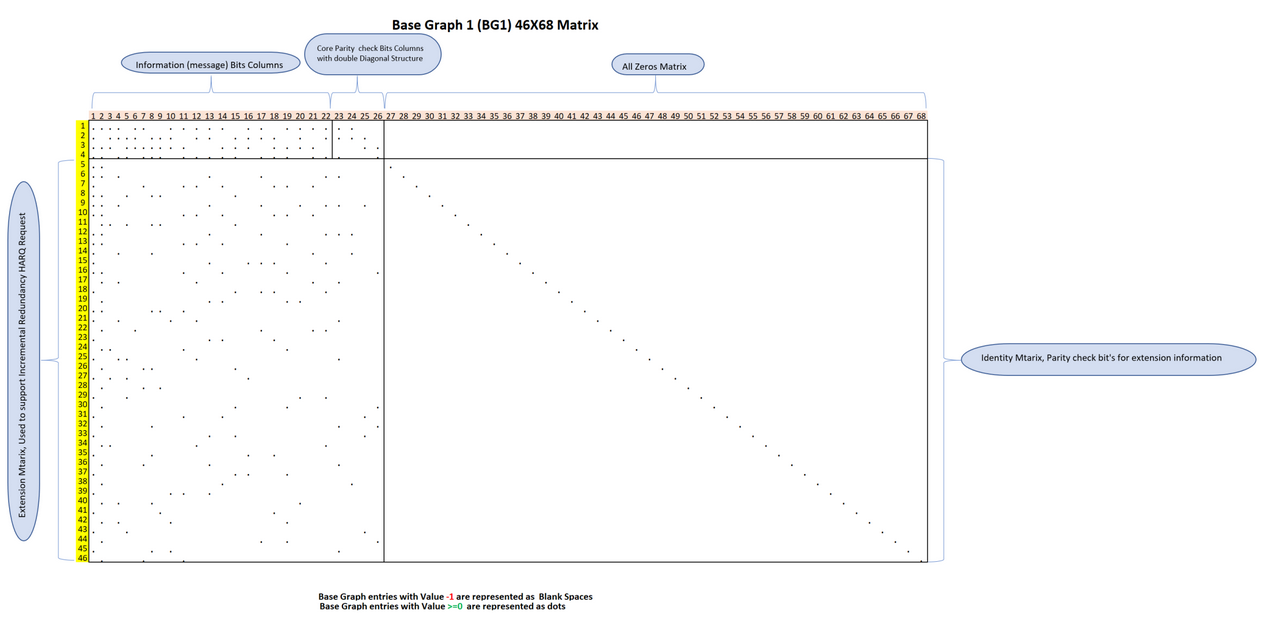
\includegraphics[width=\columnwidth]{../figs/bg1.png} 
  \caption{High Level Visualization of fully Populated BG1 Matrix}
  \end{figure}
  \item  Base Graph 2 (BG2) : With matrix size 42X52 entries For Smaller Transport Block.\\
  \begin{figure}[h]
  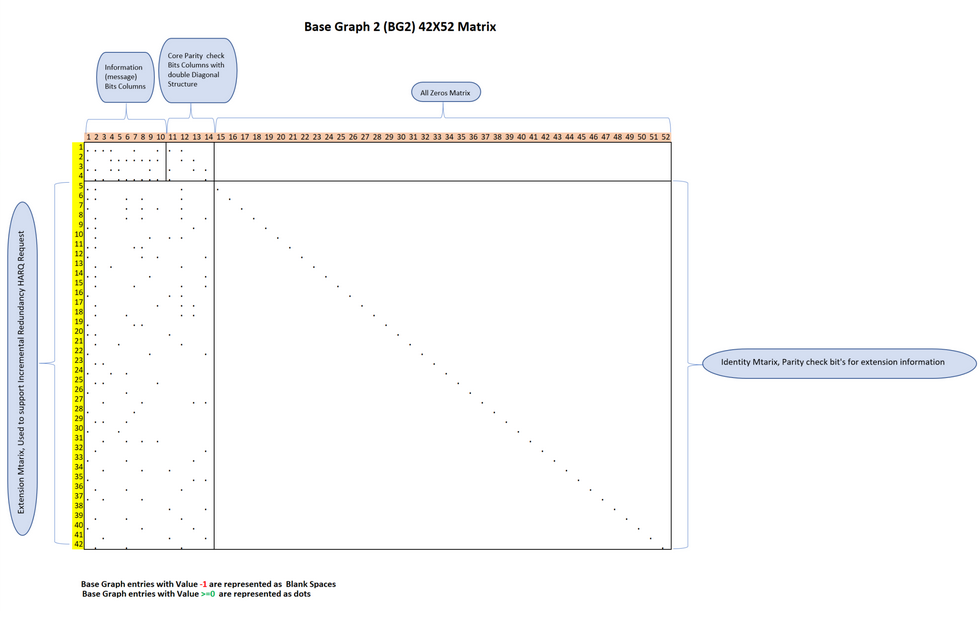
\includegraphics[width=\columnwidth]{../figs/bg2.png} 
  \caption{High Level Visualization of fully Populated BG2 Matrix}
  \end{figure}
      \end{enumerate}
      
       \subsection{\textbf{Base Graph Structure}}
The following figure represents the structure of base graph.
\vspace{15mm}
  \begin{figure}[h]
 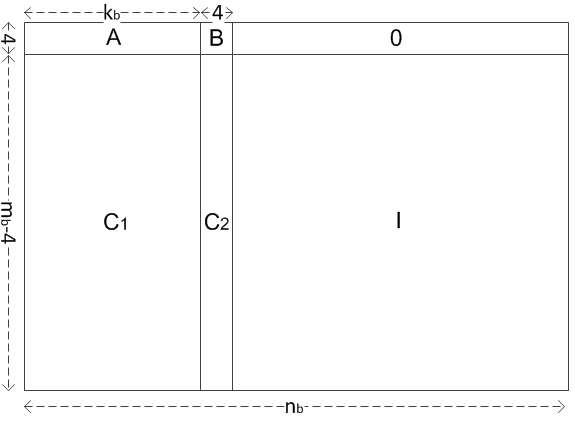
\includegraphics[width=\columnwidth]{../figs/H.png}    
     \caption{Structure of Base-Garph}
  \end{figure}\\
\vspace{5mm}
  where\\
  
 A=
$\begin{bmatrix}
a_{1,1} & a_{1,2} & \ldots & a_{1,k_{b}}\\
a_{2,1} & a_{2,2} & \ldots & a_{2,k_{b}}\\
a_{3,1} & a_{3,2} & \ldots & a_{3,k_{b}}\\
a_{4,1} & a_{4,2} & \ldots & a_{4,k_{b}}
\end{bmatrix}$\\
\vspace{5mm}

C$_{1}$=
$\begin{bmatrix}
c_{1,1} & c_{1,2} & \ldots & c_{1,k_{b}}\\
c_{2,1} & c_{2,2} & \ldots & c_{2,k_{b}}\\
c_{3,1} & c_{3,2} & \ldots & c_{3,k_{b}}\\
 \vdots & \vdots & \ddots & \vdots\\
c_{m_{b}-4,1} & c_{m_{b}-4,2} & \ldots & c_{m_{b}-4,k_{b}}\\ 
\end{bmatrix}$\\
\vspace{5mm}

C$_{2}$=
$\begin{bmatrix}
c_{1,k_{b}+1} & c_{1,k_{b}+2} &c_{1,k_{b}+3} & c_{1,k_{b}+4}\\
c_{2,k_{b}+1} & c_{2,k_{b}+2} &c_{2,k_{b}+3} & c_{2,k_{b}+4}\\
c_{3,k_{b}+1} & c_{3,k_{b}+2} &c_{3,k_{b}+3} & c_{3,k_{b}+4}\\
 \vdots & \vdots & \vdots& \vdots\\
c_{m_{b}-4,k_{b}+1} & c_{m_{b}-4,k_{b}+2} & c_{m_{b}-4,k_{b}+3} & c_{m_{b}-4,k_{b}+4}\\ 
\end{bmatrix}$
\vspace{5mm}\\ 
There are two types of B i.e.,

$B \in \{H_{BG1\_B1}, H_{BG1\_B2}, H_{BG2\_B1}, H_{BG2\_B2}\}$ in both BG1 and BG2. \\ 

 H$_{BG1\_B1}$=
$\begin{bmatrix}
1 & 0 & -1 & -1\\
0 & 0 & 0 & -1\\
-1 & -1 & 0 & 0\\
1 & -1 & -1 & 0
\end{bmatrix}$\\
\vspace{5mm}

 H$_{BG1\_B2}$=
$\begin{bmatrix}
0 & 0 & -1 & -1\\
105 & 0 & 0 & -1\\
-1 & -1 & 0 & 0\\
0 & -1 & -1 & 0
\end{bmatrix}$\\
\vspace{5mm}\\
 H$_{BG1\_B1}$ is for Zc set index iLS=(0,1,2,3,4,5,7), H$_{BG1_B2}$ is for iLS=(6).\\
\vspace{5mm}\\
 H$_{BG2\_B1}$=
$\begin{bmatrix}
0 & 0 & -1 & -1\\
-1 & 0 & 0 & -1\\
1 & -1 & 0 & 0\\
0 & -1 & -1 & 0
\end{bmatrix}$\\
\vspace{5mm}

 H$_{BG2\_B2}$=
$\begin{bmatrix}
1 & 0 & -1 & -1\\
-1 & 0 & 0 & -1\\
0 & -1 & 0 & 0\\
1 & -1 & -1 & 0
\end{bmatrix}$\\
\vspace{5mm}\\ 
  H$_{BG2\_B1}$ is for Zc set index iLS=(0,1,2,4,5,6), H$_{BG2_B2}$ is for iLS=(3,7).\\ 
  \vspace{5mm}\\
  

      
 \subsection{\textbf{LDPC Base Graph selection procedure}}   
   I have put together the following example of constructing the LDCP parity check matrix for a given information block size K and code rate R = K/N.\\
For simplicity I have considered a small TBS of size 20bits to illustrate below example, K=20 and R=0.25   
\begin{enumerate}
  \item Obtain the base graph BG1 or BG2 for the given K (Transport Block )and R (Code Rate),Refer {\href{https://www.etsi.org/deliver/etsi_ts/138200_138299/138212/17.01.00_60/ts_138212v170100p.pdf}{3GPP Specification 38.212}} for LDPC base graph selection. \\
As per the specification\\
\begin{enumerate}
 \item if K$<=$3824 and R$<=$0.67 then BG2 is selected.\\
 \item    If K$<=$ 292 then BG2 is selected\\
 \item    if R$<=$0.25 then BG2 is selected.\\
 \item    Else BG1 is selected\\
 \end{enumerate}
   \begin{figure}[h]
 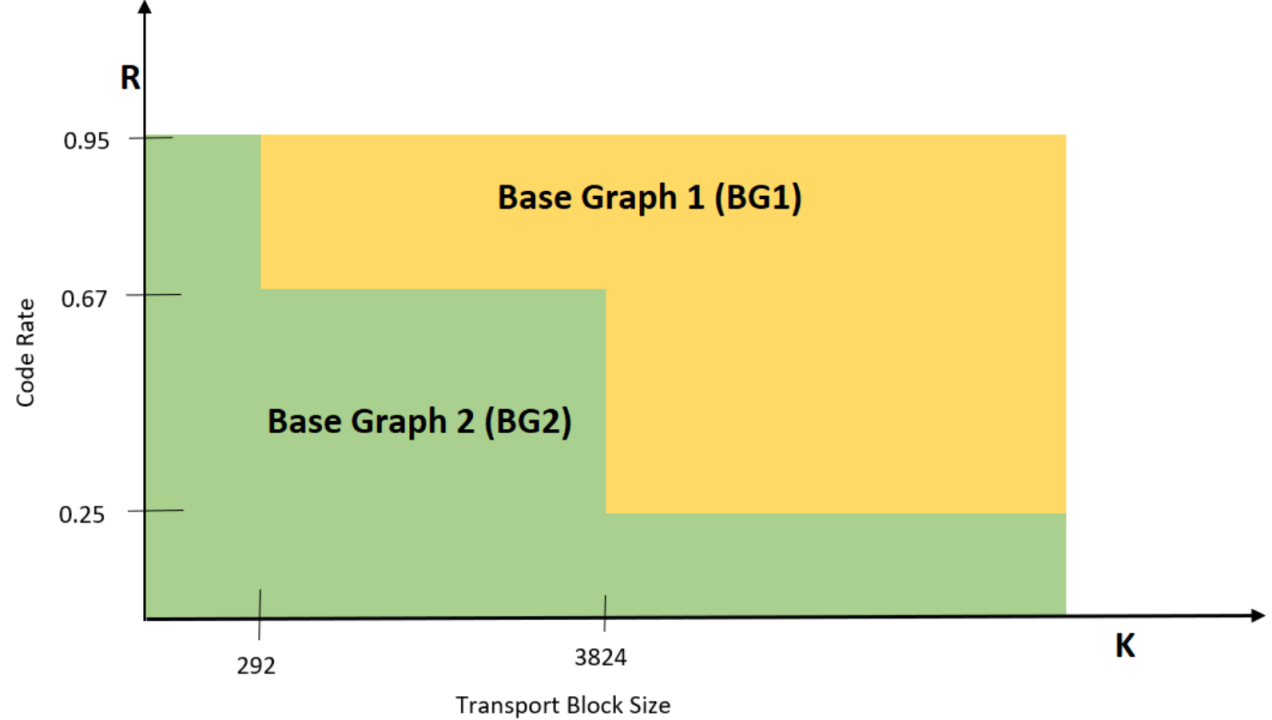
\includegraphics[width=\columnwidth]{../figs/bgs-sel.png} 
  \caption{Graphical Representation of Base Graph Selection}
  \end{figure}
    \item  Determine the value of Kb for the given K (Transport Block) and R (Code Rate) Ref {\href{https://www.etsi.org/deliver/etsi_ts/138200_138299/138212/17.01.00_60/ts_138212v170100p.pdf}{3GPP Specification 38.212, 5.2.2}}\\
    Kb denotes the number of information bit columns for the lifting size Zc.\\

As per the Specification\\

For LDPC BG1:\\
\begin{enumerate}
  \item        Kb = 22 \\
  \end{enumerate}
For LDPC BG2:\\
\begin{enumerate}
 \item     if K is between 640 $<$ K $<=$ 3824 then Kb = 10\\
  \item    if K is between 560 $<$ K $<=$ 640 then Kb = 9\\
  \item    if K is between 192 $<$ K $<=$ 560 then Kb =8\\
  \item    If K is $<=$ 192 then Kb is = 6\\
    \end{enumerate}
    
 \item  Determine the base matrix expansion factor Zc by selecting the minimum Zc value in below Table,such that Kb*Zc $>=$K.Sets of LDPC lifting size Zc in the specification I have populated below Zc table.\\
\begin{centering}
a\\
\end{centering}
\begin{centering}
j
\end{centering}
     \begin{tabular} {|>{\columncolor{red!35}} p {0.3 cm} | p {0.4 cm} | p {0.4 cm} | p {0.4 cm} | p {0.4 cm} | p {0.4 cm} | p {0.4 cm} | p {0.4 cm} | p {0.4 cm} |  }
         \hline
        \rowcolor{orange!80}    \cellcolor{blue!30}Zc & 2 &3 &5 &7 &9 &11 &13 &15\\
    \hline
     0 &\cellcolor{blue!30} 2 &\cellcolor{blue!30}3 &\cellcolor{blue!30}5 &\cellcolor{blue!30}7 &\cellcolor{blue!30}9 &\cellcolor{blue!30}11 &\cellcolor{blue!30}13 &\cellcolor{blue!30}15 \\
    \hline
   1 &\cellcolor{blue!30} 4 &\cellcolor{blue!30}6 &\cellcolor{blue!30}10 &\cellcolor{blue!30}14 &\cellcolor{blue!30}18 &\cellcolor{blue!30}22 &\cellcolor{blue!30}26 &\cellcolor{blue!30}30\\
   \hline
    2 & \cellcolor{blue!30}8 &\cellcolor{blue!30}12 &\cellcolor{blue!30}20 &\cellcolor{blue!30}28 &\cellcolor{blue!30}36 &\cellcolor{blue!30}44 &\cellcolor{blue!30}52 &\cellcolor{blue!30}60 \\
    \hline
   3 & \cellcolor{blue!30}16 &\cellcolor{blue!30}24 &\cellcolor{blue!30}40 &\cellcolor{blue!30}56 &\cellcolor{blue!30}72 &\cellcolor{blue!30}88 &\cellcolor{blue!30}104 &\cellcolor{blue!30}120 \\
    \hline
     4 & \cellcolor{blue!30}32 &\cellcolor{blue!30}48 &\cellcolor{blue!30}80 &\cellcolor{blue!30}112 &\cellcolor{blue!30}144 &\cellcolor{blue!30}196 &\cellcolor{blue!30}208 &\cellcolor{blue!30}240\\
    \hline
     5 &\cellcolor{blue!30} 64 &\cellcolor{blue!30}96 &\cellcolor{blue!30}160 &\cellcolor{blue!30}224 &\cellcolor{blue!30}288 &\cellcolor{blue!30} & \cellcolor{blue!30}&\cellcolor{blue!30}\\
    \hline
     6 &\cellcolor{blue!30} 128 &\cellcolor{blue!30}192 &\cellcolor{blue!30}320 &\cellcolor{blue!30} &\cellcolor{blue!30} &\cellcolor{blue!30} &\cellcolor{blue!30} &\cellcolor{blue!30}\\
    \hline
     7 &\cellcolor{blue!30} 256 &\cellcolor{blue!30}384 &\cellcolor{blue!30} &\cellcolor{blue!30} &\cellcolor{blue!30} &\cellcolor{blue!30} & \cellcolor{blue!30}&\cellcolor{blue!30}\\
    \hline
    \end{tabular}\\
    Zc=a*2\textsuperscript{j}\\
  
          
          
       For K=20 , Zc = 4, this satisfies the condition Kb*Zc $>$= K , 6*4 = 24 , 24$>$ 20 and this is the minimum Zc value from the above table that satisfies this condition.\\
    \item       After Zc is determined, the corresponding shift coefficient matrix set need to be selected from below Table., Ref for this table is    {\href{https://www.etsi.org/deliver/etsi_ts/138200_138299/138212/17.01.00_60/ts_138212v170100p.pdf}{3GPP Specification 38.212,5.3.2 }}\\
     \vspace{4mm}
     
       \begin{tabular} {| p {2.1 cm} | p {4 cm} |}
       \hline
  
  \cellcolor{violet!40} Set Index(iLS)& \cellcolor{violet!40}Set of Lifting Sizes(Zc)\\
  \hline
  
  0&2,4,8,16,32,64,128,256\\
  \hline
    1&3,6,12,24,48,96,192,384\\
  \hline
     2&5,10,20,40,80,160,320\\
  \hline
     3&7,14,28,56,112,224\\
  \hline
    4&9,18,36,72,144,288\\
  \hline
    5&11,22,44,88,196\\
  \hline
    6&13,26,52,104,208\\
  \hline
   7&15,30,60,120,240\\
  \hline
    \end{tabular}\\  
    
    Since Zc = 4, Set Index (iLS) "0" is considered.\\
    
   \item      Determine the entries values in the base matrix based on the Zc,  Calculate the shifting coefficient value P(i,j) by the modular Zc operation. 
   
   \begin{lstlisting}
    P(i,j)= f(Vi,j , Zc)= mod(Vi,j, Zc)
    \end{lstlisting}
    Referral tables to calculate P(i,j) are available in the specification {\href{https://www.etsi.org/deliver/etsi_ts/138200_138299/138212/17.01.00_60/ts_138212v170100p.pdf}{3GPP Specification 38.212,5.3.2 }}\\
  \begin{figure}[h]
 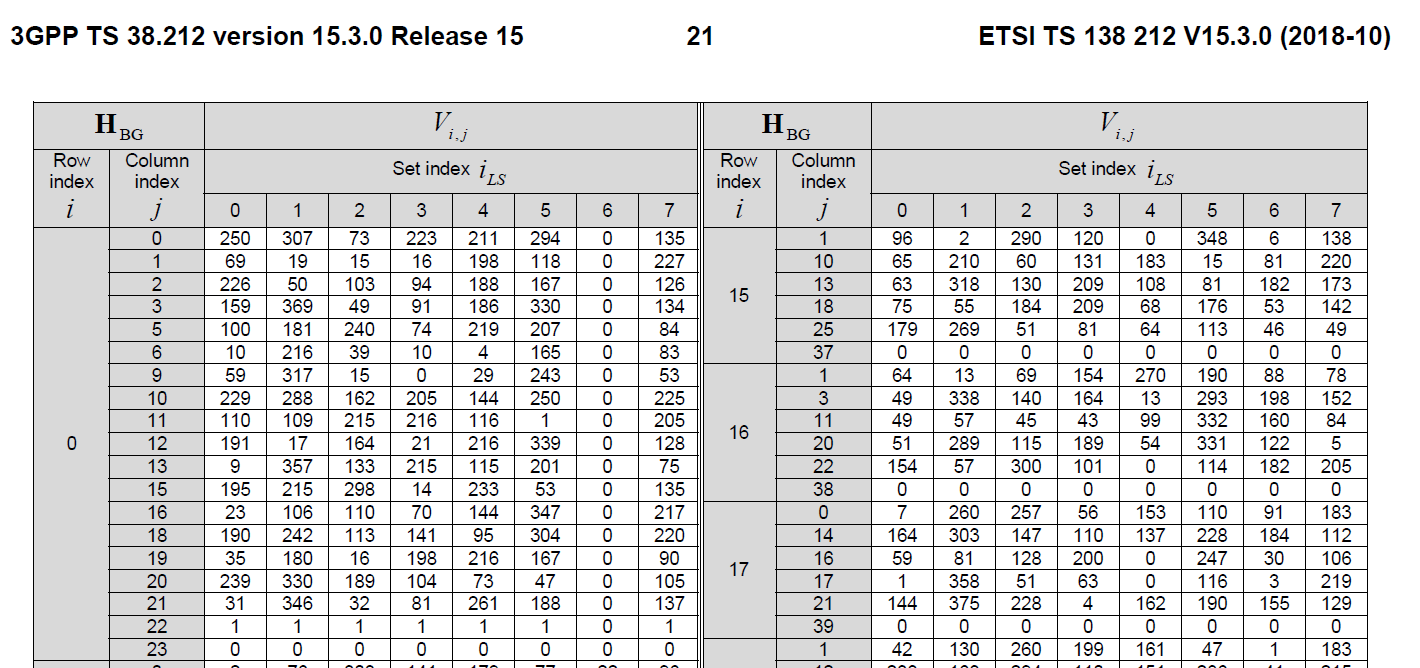
\includegraphics[width=\columnwidth]{../figs/hbgtab1.png}    
     \caption{LDPC base graph 1 (BG 1) and its parity check matrices}
  \end{figure}\\
  \vspace{5mm}
    \begin{figure}[h]
 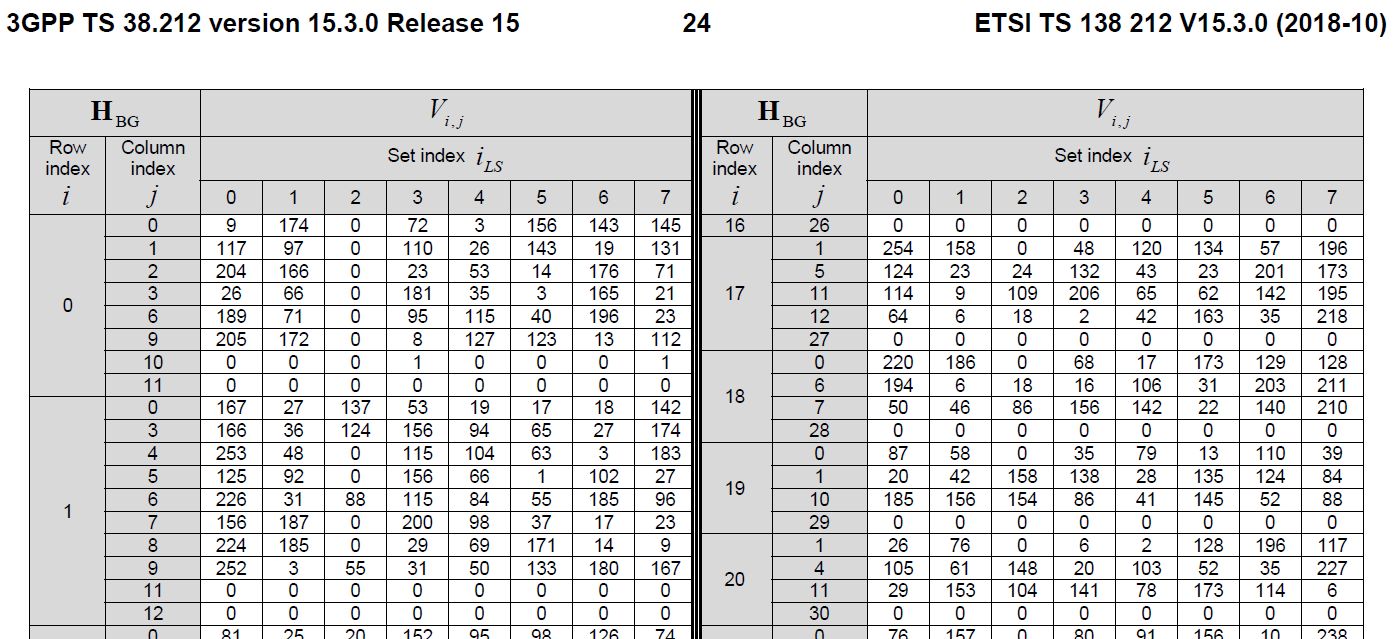
\includegraphics[width=\columnwidth]{../figs/hbgtab2.png}    
     \caption{LDPC base graph 2 (BG 2) and its parity check matrices}
  \end{figure}\\
For K=20 , Base Graph = 2, Zc= 4 and SetIndex  iLS = 0, from above Table LDPC base graph 2 Using the equation P(i,j) = f(Vi,j , z) = mod(Vi,j , z) all the possible base graph matrix entries with the shifting coefficient are determined.   \\
Below I have illustrated how the Base Matrix entries P(i.j) are populated, I have considered only the first row for below illustration, like wise the full matrix is built.\\
 \begin{figure}[h]
 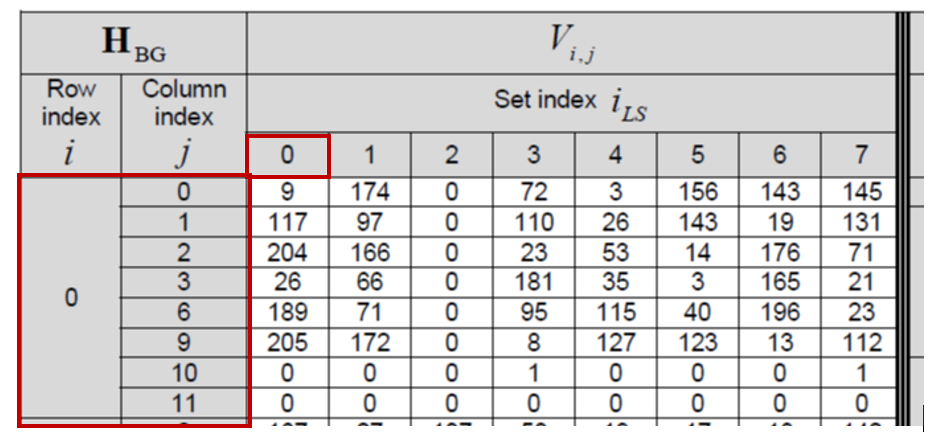
\includegraphics[width=\columnwidth]{../figs/selbgs.png}    
     \caption{LDPC parity check matrix selection}
  \end{figure}\\
  From Step 3 and 4 Set Index iLS = 0 and Zc =4\\
   \begin{figure}[h]
 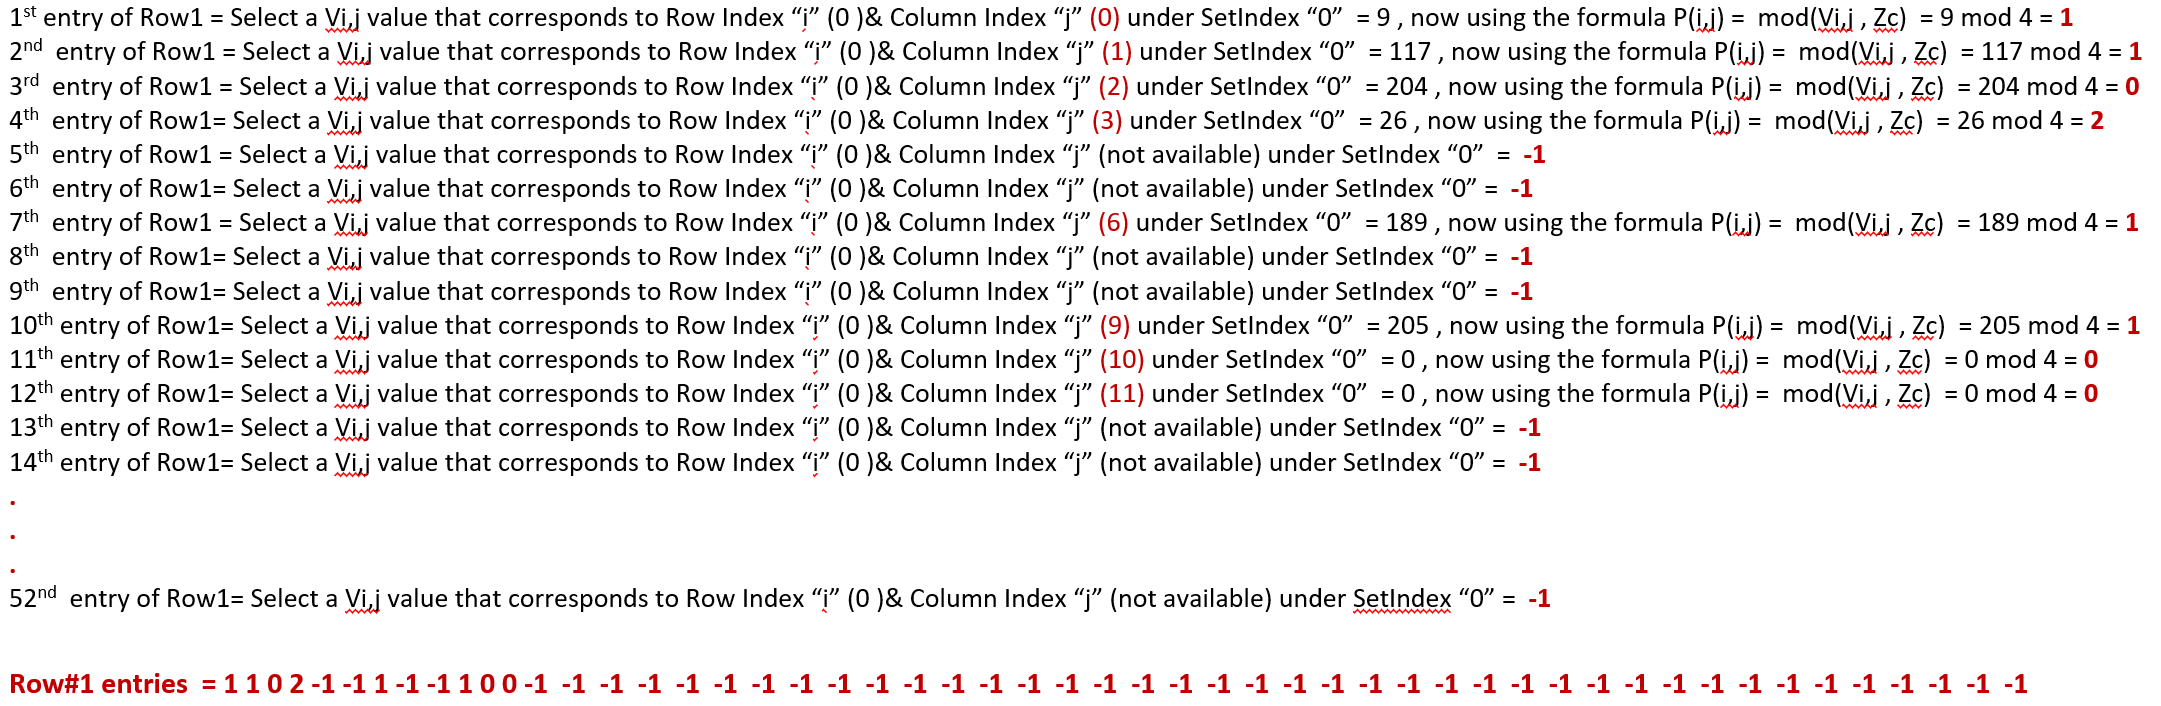
\includegraphics[width=\columnwidth]{../figs/mod.png}    
     \caption{modulus operation}
  \end{figure}\\
  
  Using the above principal remaining all entries of the matrix can be populated based on the Row index i and Column Index j and SetIndex(iLS)\\
  I populated the below full base graph2 matrix with Zc=4\\
  \vspace{5mm}
     \begin{figure}[h]
 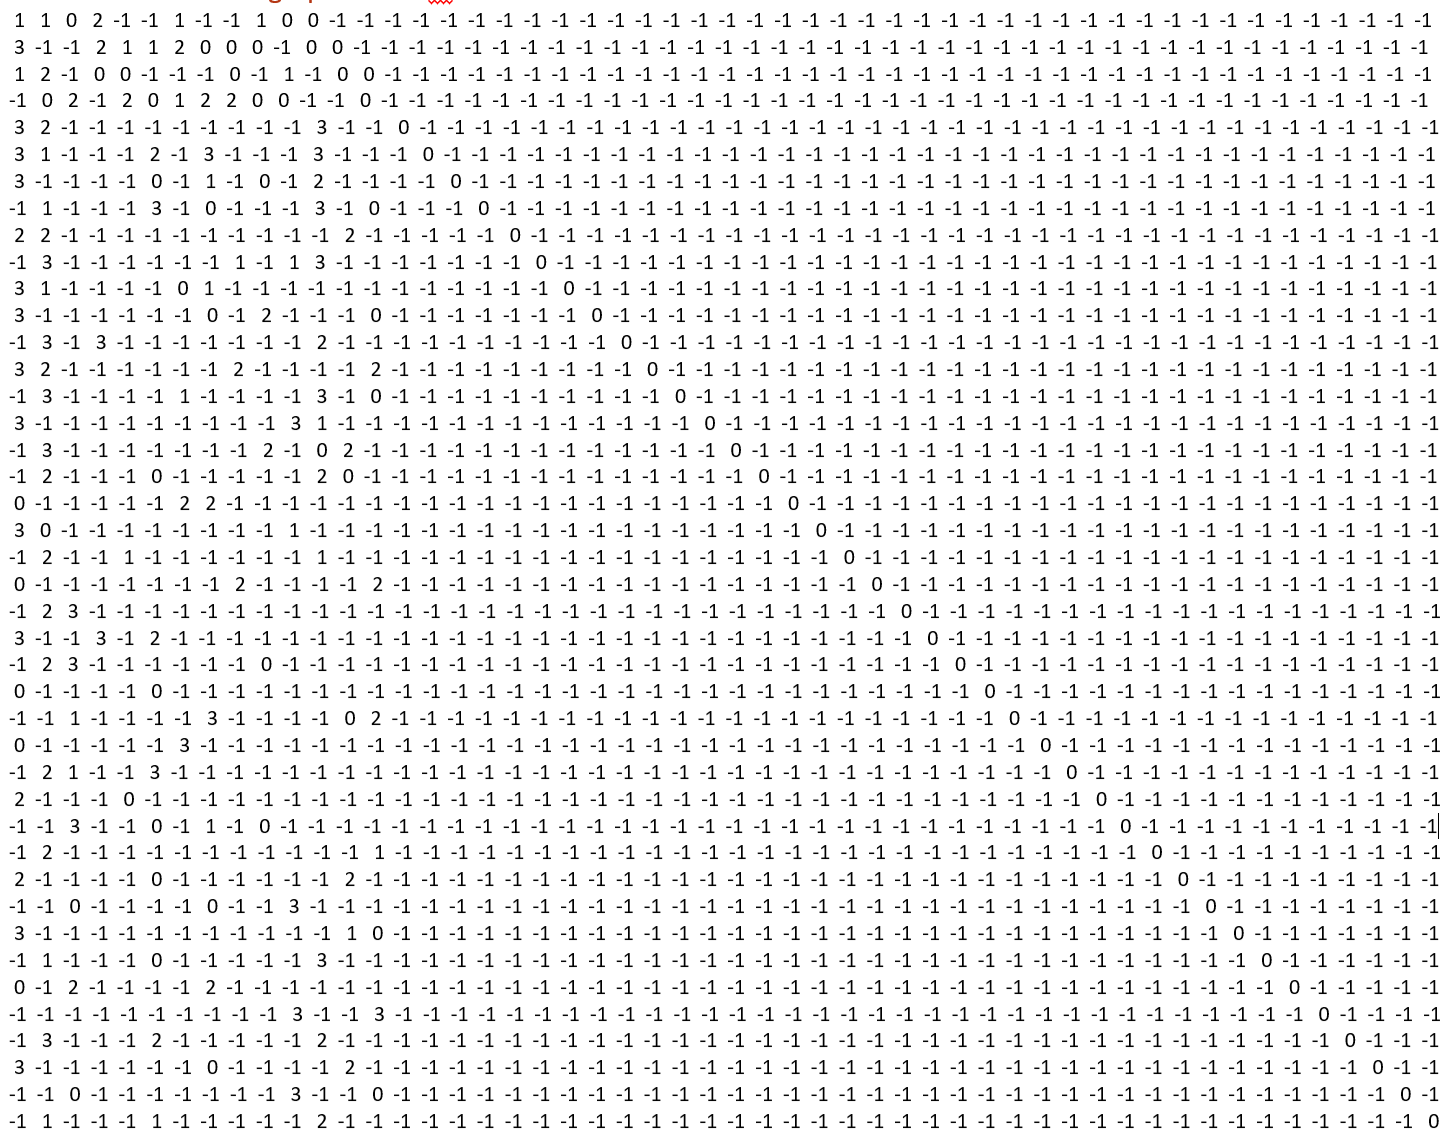
\includegraphics[width=\columnwidth]{../figs/pcm.png}    
     \caption{Base Graph2 for iLS=0 and Zc=4}
  \end{figure}\\
  
  The above mentioned steps are used in the following program to generate base graphs based on K and N.\\
   \begin{center}
     \fbox {\href{https://github.com/KrishnaYadati/IIT-H-FWC-Project/blob/main/5G-NR-LDPC-Encoder/codes/ldpcbasegraphgen.c}{ldpcbasegraphgen.c}}
       \end{center}
      \vspace{2mm}  
I have generated all the posible base graphs and are available in {\href{https://github.com/KrishnaYadati/IIT-H-FWC-Project/tree/main/5G-NR-LDPC-Encoder/Base_Graphs}{BaseGraphs}} section .\\
 
 \subsection{\textbf{Encoding Algorithm}} 
   Let the codeword be\\
 
C=[s$_{1}$,s$_{2}$,....s$_{k_b}$,p$_{b_1}$,p$_{b_2}$,p$_{b_3}$,p$_{b_4}$,p$_{c_1}$,p$_{c_2}$,.....,p$_{c_{m_{b}-4}}$]\\

where each element of C is a vector of length Zc. \\
The encoding of LDPC codes is carried out as follows:\\

 
  \begin{enumerate} 
 \item First step is to generate any random message of size equal to lifting size (Zc) which has obtained during the selection of base graph.Then Zc should be multiplied with the original information bits i.e., difference between rows and columns for the selected base graph.\\
  \begin{lstlisting}
  Zc * (Column Size-Row Size)
 \end{lstlisting}
 \vspace{5mm}
   \item After that generate the codeword.Which should be of size given below \\
  \begin{lstlisting}
  Zc * Column Size
 \end{lstlisting}
 
  \end{enumerate} 

            \end{enumerate} 
      
         
\end{document}

\chapter{Random Numbers}
\iffalse
\let\negmedspace\undefined
\let\negthickspace\undefined
\documentclass[journal,12pt,twocolumn]{IEEEtran}
%\documentclass[conference]{IEEEtran}
%\IEEEoverridecommandlockouts
% The preceding line is only needed to identify funding in the first footnote. If that is unneeded, please comment it out.
\usepackage{cite}
\usepackage{amssymb,amsfonts,amsthm,amsmath}
\usepackage{algorithmic}
\usepackage{graphicx}
\usepackage{textcomp}
\usepackage{xcolor}
\usepackage{txfonts}
\usepackage{listings}
\usepackage{enumitem}
\usepackage{mathtools}
\usepackage{gensymb}

%%
%\usepackage{setspace}
%%\doublespacing
%\singlespacing
%
%%\usepackage{graphicx}
%%\usepackage{amssymb}
%%\usepackage{relsize}
%\usepackage[cmex10]{amsmath}
%%\interdisplaylinepenalty=2500
%%\savesymbol{iint}
%%\usepackage{txfonts}
%%\restoresymbol{TXF}{iint}
%%\usepackage{wasysym}
%\usepackage{amsthm}
%\usepackage{mathrsfs}
%\usepackage{txfonts}
%%\usepackage{stfloats}
%%\usepackage{cite}
%%\usepackage{cases}
%%\usepackage{subfig}
%%\usepackage{xtab}
%%\usepackage{multirow}
%%\usepackage{algorithm}
%%\usepackage{algpseudocode}
%%\usepackage{tikz}
%%\usepackage{circuitikz}
%%\usepackage{verbatim}
\usepackage{hyperref}
%%\usepackage{stmaryrd}
%%\usepackage{tkz-euclide} % loads  TikZ and tkz-base
%%\usetkzobj{all}
    \usepackage{color}                                            %%
    \usepackage{array}                                            %%
    \usepackage{longtable}                                        %%
    \usepackage{calc}                                             %%
    \usepackage{multirow}                                         %%
    \usepackage{hhline}                                           %%
    \usepackage{ifthen}                                           %%
%  %optionally (for landscape tables embedded in another document): %%
%    \usepackage{lscape}     
%%\usepackage{multicol}
%\usepackage{chngcntr}
%\usepackage{enumerate}

%\usepackage{wasysym}
%\newcounter{MYtempeqncnt}
\DeclareMathOperator*{\Res}{Res}
%\renewcommand{\baselinestretch}{2}
\renewcommand\thesection{\arabic{section}}
\renewcommand\thesubsection{\thesection.\arabic{subsection}}
\renewcommand\thesubsubsection{\thesubsection.\arabic{subsubsection}}

\renewcommand\thesectiondis{\arabic{section}}
\renewcommand\thesubsectiondis{\thesectiondis.\arabic{subsection}}
\renewcommand\thesubsubsectiondis{\thesubsectiondis.\arabic{subsubsection}}

% correct bad hyphenation here
\hyphenation{op-tical net-works semi-conduc-tor}
\def\inputGnumericTable{}                                 %%

\lstset{
language=tex,
frame=single, 
breaklines=true
}

\begin{document}
%


\newtheorem{theorem}{Theorem}[section]
\newtheorem{problem}{Problem}
\newtheorem{proposition}{Proposition}[section]
\newtheorem{lemma}{Lemma}[section]
\newtheorem{corollary}[theorem]{Corollary}
\newtheorem{example}{Example}[section]
\newtheorem{definition}[problem]{Definition}
%\newtheorem{thm}{Theorem}[section] 
%\newtheorem{defn}[thm]{Definition}
%\newtheorem{algorithm}{Algorithm}[section]
%\newtheorem{cor}{Corollary}
\newcommand{\BEQA}{\begin{eqnarray}}
\newcommand{\EEQA}{\end{eqnarray}}
\newcommand{\define}{\stackrel{\triangle}{=}}
\bibliographystyle{IEEEtran}
%\bibliographystyle{ieeetr}
\providecommand{\mbf}{\mathbf}
\providecommand{\pr}[1]{\ensuremath{\Pr\left(#1\right)}}
\providecommand{\re}[1]{\ensuremath{\text{Re}\left(#1\right)}}
\providecommand{\im}[1]{\ensuremath{\text{Im}\left(#1\right)}}
\providecommand{\qfunc}[1]{\ensuremath{Q\left(#1\right)}}
\providecommand{\sbrak}[1]{\ensuremath{{}\left[#1\right]}}
\providecommand{\lsbrak}[1]{\ensuremath{{}\left[#1\right.}}
\providecommand{\rsbrak}[1]{\ensuremath{{}\left.#1\right]}}
\providecommand{\brak}[1]{\ensuremath{\left(#1\right)}}
\providecommand{\lbrak}[1]{\ensuremath{\left(#1\right.}}
\providecommand{\rbrak}[1]{\ensuremath{\left.#1\right)}}
\providecommand{\cbrak}[1]{\ensuremath{\left\{#1\right\}}}
\providecommand{\lcbrak}[1]{\ensuremath{\left\{#1\right.}}
\providecommand{\rcbrak}[1]{\ensuremath{\left.#1\right\}}}
\theoremstyle{remark}
\newtheorem{rem}{Remark}
\newcommand{\sgn}{\mathop{\mathrm{sgn}}}
\providecommand{\abs}[1]{\left\vert#1\right\vert}
\providecommand{\res}[1]{\Res\displaylimits_{#1}} 
\providecommand{\norm}[1]{\left\lVert#1\right\rVert}
%\providecommand{\norm}[1]{\lVert#1\rVert}
\providecommand{\mtx}[1]{\mathbf{#1}}
\providecommand{\mean}[1]{E\left[ #1 \right]}
\providecommand{\fourier}{\overset{\mathcal{F}}{ \rightleftharpoons}}
%\providecommand{\hilbert}{\overset{\mathcal{H}}{ \rightleftharpoons}}
\providecommand{\system}{\overset{\mathcal{H}}{ \longleftrightarrow}}
	%\newcommand{\solution}[2]{\textbf{Solution:}{#1}}
\newcommand{\solution}{\noindent \textbf{Solution: }}
\providecommand{\dec}[2]{\ensuremath{\overset{#1}{\underset{#2}{\gtrless}}}}
\newcommand{\myvec}[1]{\ensuremath{\begin{pmatrix}#1\end{pmatrix}}}
\newcommand{\mydet}[1]{\ensuremath{\begin{vmatrix}#1\end{vmatrix}}}
	\newcommand*{\permcomb}[4][0mu]{{{}^{#3}\mkern#1#2_{#4}}}
\newcommand*{\perm}[1][-3mu]{\permcomb[#1]{P}}
\newcommand*{\comb}[1][-1mu]{\permcomb[#1]{C}}
\providecommand{\gauss}[2]{\mathcal{N}\ensuremath{\left(#1,#2\right)}}
%%
%	%\newcommand{\solution}[2]{\textbf{Solution:}{#1}}
%\newcommand{\solution}{\noindent \textbf{Solution: }}
\newcommand{\cosec}{\,\text{cosec}\,}
\newcommand{\sinc}{\,\text{sinc}\,}
\newcommand{\rect}{\,\text{rect}\,}
%\numberwithin{equation}{section}
\numberwithin{equation}{subsection}
%\numberwithin{problem}{section}
%\numberwithin{definition}{section}
\makeatletter
\@addtoreset{figure}{problem}
\makeatother
\let\StandardTheFigure\thefigure
\let\vec\mathbf
\let\j\jmath
%\renewcommand{\thefigure}{\theproblem.\arabic{figure}}
\renewcommand{\thefigure}{\theproblem}
%\setlist[enumerate,1]{before=\renewcommand\theequation{\theenumi.\arabic{equation}}
%\counterwithin{equation}{enumi}
%\renewcommand{\theequation}{\arabic{subsection}.\arabic{equation}}
\def\putbox#1#2#3{\makebox[0in][l]{\makebox[#1][l]{}\raisebox{\baselineskip}[0in][0in]{\raisebox{#2}[0in][0in]{#3}}}}
     \def\rightbox#1{\makebox[0in][r]{#1}}
     \def\centbox#1{\makebox[0in]{#1}}
     \def\topbox#1{\raisebox{-\baselineskip}[0in][0in]{#1}}
     \def\midbox#1{\raisebox{-0.5\baselineskip}[0in][0in]{#1}}
\vspace{3cm}
\title{
%	\logo{
	Probability
%	}
}
%\title{
%	\logo{Matrix Analysis through Octave}{\begin{center}\includegraphics[scale=.24]{tlc}\end{center}}{}{HAMDSP}
%}
% paper title
% can use linebreaks \\ within to get better formatting as desired
%\title{Matrix Analysis through Octave}
%
%
% author names and IEEE memberships
% note positions of commas and nonbreaking spaces ( ~ ) LaTeX will not break
% a structure at a ~ so this keeps an author's name from being broken across
% two lines.
% use \thanks{} to gain access to the first footnote area
% a separate \thanks must be used for each paragraph as LaTeX2e's \thanks
% was not built to handle multiple paragraphs
%
\author{
	G. V. V. Sharma
	%<-this % stops a space
%\thanks{}}
}
% note the % following the last \IEEEmembership and also \thanks - 
% these prevent an unwanted space from occurring between the last author name
% and the end of the author line. i.e., if you had this:
% 
% \author{....lastname \thanks{...} \thanks{...} }
%                     ^------------^------------^----Do not want these spaces!
%
% a space would be appended to the last name and could cause every name on that
% line to be shifted left slightly. This is one of those "LaTeX things". For
% instance, "\textbf{A} \textbf{B}" will typeset as "A B" not "AB". To get
% "AB" then you have to do: "\textbf{A}\textbf{B}"
% \thanks is no different in this regard, so shield the last } of each \thanks
% that ends a line with a % and do not let a space in before the next \thanks.
% Spaces after \IEEEmembership other than the last one are OK (and needed) as
% you are supposed to have spaces between the names. For what it is worth,
% this is a minor point as most people would not even notice if the said evil
% space somehow managed to creep in.
% The paper headers
%\markboth{Journal of \LaTeX\ Class Files,~Vol.~6, No.~1, January~2007}%
%{Shell \MakeLowercase{\textit{et al.}}: Bare Demo of IEEEtran.cls for Journals}
% The only time the second header will appear is for the odd numbered pages
% after the title page when using the twoside option.
% 
% *** Note that you probably will NOT want to include the author's ***
% *** name in the headers of peer review papers.                   ***
% You can use \ifCLASSOPTIONpeerreview for conditional compilation here if
% you desire.
% If you want to put a publisher's ID mark on the page you can do it like
% this:
%\IEEEpubid{0000--0000/00\$00.00~\copyright~2007 IEEE}
% Remember, if you use this you must call \IEEEpubidadjcol in the second
% column for its text to clear the IEEEpubid mark.
% make the title area
\maketitle
\newpage
\tableofcontents
\bigskip
\renewcommand{\thefigure}{\theenumi}
\renewcommand{\thetable}{\theenumi}
%\renewcommand{\theequation}{\theenumi}
%\begin{abstract}
%%\boldmath
%In this letter, an algorithm for evaluating the exact analytical bit error rate  (BER)  for the piecewise linear (PL) combiner for  multiple relays is presented. Previous results were available only for upto three relays. The algorithm is unique in the sense that  the actual mathematical expressions, that are prohibitively large, need not be explicitly obtained. The diversity gain due to multiple relays is shown through plots of the analytical BER, well supported by simulations. 
%
%\end{abstract}
% IEEEtran.cls defaults to using nonbold math in the Abstract.
% This preserves the distinction between vectors and scalars. However,
% if the journal you are submitting to favors bold math in the abstract,
% then you can use LaTeX's standard command \boldmath at the very start
% of the abstract to achieve this. Many IEEE journals frown on math
% in the abstract anyway.
% Note that keywords are not normally used for peerreview papers.
%\begin{IEEEkeywords}
%Cooperative diversity, decode and forward, piecewise linear
%\end{IEEEkeywords}
% For peer review papers, you can put extra information on the cover
% page as needed:
% \ifCLASSOPTIONpeerreview
% \begin{center} \bfseries EDICS Category: 3-BBND \end{center}
% \fi
%
% For peerreview papers, this IEEEtran command inserts a page break and
% creates the second title. It will be ignored for other modes.
%\IEEEpeerreviewmaketitle
%\begin{abstract}
%\end{abstract}
%\iffalse
%% Copyright (C) 2020 Saurabh Joshi
%%% 
%\let\negmedspace\undefined
%\let\negthickspace\undefined
%
%\documentclass[journal,12pt,onecolumn]{IEEEtran}
%%\documentclass[journal,12pt,twocolumn]{IEEEtran}
%%
%\usepackage{setspace}
%\usepackage{gensymb}
%%\doublespacing
%\singlespacing
%
%%\usepackage{graphicx}
%%\usepackage{amssymb}
%%\usepackage{relsize}
%\usepackage[cmex10]{amsmath}
%%\usepackage{amsthm}
%%\interdisplaylinepenalty=2500
%%\savesymbol{iint}
%%\usepackage{txfonts}
%%\restoresymbol{TXF}{iint}
%%\usepackage{wasysym}
%\usepackage{amsthm}
%\usepackage{mathrsfs}
%\usepackage{txfonts}
%\usepackage{stfloats}
%\usepackage{cite}
%\usepackage{cases}
%\usepackage{subfig}
%%\usepackage{xtab}
%\usepackage{longtable}
%\usepackage{multirow}
%%\usepackage{algorithm}
%%\usepackage{algpseudocode}
%\usepackage{enumitem}
%\usepackage{mathtools}
%\usepackage{tikz}
%\usepackage{circuitikz}
%\usepackage{verbatim}
%\usepackage{hyperref}
%%\usepackage{stmaryrd}
%\usepackage{tkz-euclide} % loads  TikZ and tkz-base
%%\usetkzobj{all}
%\usepackage{listings}
%    \usepackage{color}                                            %%
%    \usepackage{array}                                            %%
%    \usepackage{longtable}                                        %%
%    \usepackage{calc}                                             %%
%    \usepackage{multirow}                                         %%
%    \usepackage{hhline}                                           %%
%    \usepackage{ifthen}                                           %%
%  %optionally (for landscape tables embedded in another document): %%
%    \usepackage{lscape}     
%\usepackage{multicol}
%\usepackage{chngcntr}
%\usepackage{iftex}
%%\usepackage[latin9]{inputenc}
%\usepackage{geometry}
%\usepackage{bm}
%%\geometry{verbose,tmargin=2cm,bmargin=3cm,lmargin=1.8cm,rmargin=1.5cm,headheight=2cm,headsep=2cm,footskip=3cm}
%\usepackage{array}
%\newcolumntype{L}[1]{>{\raggedright\let\newline\\\arraybackslash\hspace{0pt}}m{#1}}
%\newcolumntype{C}[1]{>{\centering\let\newline\\\arraybackslash\hspace{0pt}}m{#1}}
%\newcolumntype{R}[1]{>{\raggedleft\let\newline\\\arraybackslash\hspace{0pt}}m{#1}}
%
%%\usepackage{graphicx}
%%\usepackage{setspace}
%%\usepackage{parskip}
%
%\def \hsp {\hspace{3mm}}
%
%\makeatletter
%
%\providecommand{\tabularnewline}{\\}
%
%
%
%\makeatother
%\ifxetex
%\usepackage[T1]{fontenc}
%\usepackage{fontspec}
%%\setmainfont[ Path = fonts/]{Sanskrit_2003.ttf}
%\newfontfamily\nakulafont[Script=Devanagari,AutoFakeBold=2,Path = fonts/]{Nakula}
%%\newfontfamily\liberationfont{Liberation Sans Narrow}
%%\newfontfamily\liberationsansfont{Liberation Sans}
%\fi
%\usepackage{tikz}
%\usepackage{xcolor}
%%\usepackage{enumerate}
%
%%\usepackage{wasysym}
%%\newcounter{MYtempeqncnt}
%\DeclareMathOperator*{\Res}{Res}
%%\renewcommand{\baselinestretch}{2}
%\renewcommand\thesection{\arabic{section}}
%\renewcommand\thesubsection{\thesection.\arabic{subsection}}
%\renewcommand\thesubsubsection{\thesubsection.\arabic{subsubsection}}
%
%\renewcommand\thesectiondis{\arabic{section}}
%\renewcommand\thesubsectiondis{\thesectiondis.\arabic{subsection}}
%\renewcommand\thesubsubsectiondis{\thesubsectiondis.\arabic{subsubsection}}
%
%% correct bad hyphenation here
%\hyphenation{op-tical net-works semi-conduc-tor}
%\def\inputGnumericTable{}                                 %%
%
%\lstset{
%language=tex,
%frame=single, 
%breaklines=true
%}
%
%%\begin{document}
%%
%
%
%\newtheorem{theorem}{Theorem}[section]
%\newtheorem{problem}{Problem}
%\newtheorem{proposition}{Proposition}[section]
%\newtheorem{lemma}{Lemma}[section]
%\newtheorem{corollary}[theorem]{Corollary}
%\newtheorem{example}{Example}[section]
%\newtheorem{definition}[problem]{Definition}
%%\newtheorem{thm}{Theorem}[section] 
%%\newtheorem{defn}[thm]{Definition}
%%\newtheorem{algorithm}{Algorithm}[section]
%%\newtheorem{cor}{Corollary}
%\newcommand{\BEQA}{\begin{eqnarray}}
%\newcommand{\EEQA}{\end{eqnarray}}
%\newcommand{\define}{\stackrel{\triangle}{=}}
%
%\bibliographystyle{IEEEtran}
%%\bibliographystyle{ieeetr}
%
%
%\providecommand{\mbf}{\mathbf}
%\providecommand{\pr}[1]{\ensuremath{\Pr\left(#1\right)}}
%\providecommand{\qfunc}[1]{\ensuremath{Q\left(#1\right)}}
%\providecommand{\sbrak}[1]{\ensuremath{{}\left[#1\right]}}
%\providecommand{\lsbrak}[1]{\ensuremath{{}\left[#1\right.}}
%\providecommand{\rsbrak}[1]{\ensuremath{{}\left.#1\right]}}
%\providecommand{\brak}[1]{\ensuremath{\left(#1\right)}}
%\providecommand{\lbrak}[1]{\ensuremath{\left(#1\right.}}
%\providecommand{\rbrak}[1]{\ensuremath{\left.#1\right)}}
%\providecommand{\cbrak}[1]{\ensuremath{\left\{#1\right\}}}
%\providecommand{\lcbrak}[1]{\ensuremath{\left\{#1\right.}}
%\providecommand{\rcbrak}[1]{\ensuremath{\left.#1\right\}}}
%\theoremstyle{remark}
%\newtheorem{rem}{Remark}
%\newcommand{\sgn}{\mathop{\mathrm{sgn}}}
%\providecommand{\abs}[1]{\left\vert#1\right\vert}
%\providecommand{\res}[1]{\Res\displaylimits_{#1}} 
%\providecommand{\norm}[1]{\left\lVert#1\right\rVert}
%%\providecommand{\norm}[1]{\lVert#1\rVert}
%\providecommand{\mtx}[1]{\mathbf{#1}}
%\providecommand{\mean}[1]{E\left[ #1 \right]}
%%\numberwithin{equation}{section}
%\numberwithin{equation}{section}
%%\numberwithin{problem}{section}
%%\numberwithin{definition}{section}
%\makeatletter
%\@addtoreset{figure}{problem}
%\makeatother
%
%\let\StandardTheFigure\thefigure
%\let\vec\mathbf
%%\renewcommand{\thefigure}{\theproblem.\arabic{figure}}
%\renewcommand{\thefigure}{\theproblem}
%%\setlist[enumerate,1]{before=\renewcommand\theequation{\theenumi.\arabic{equation}}
%%\counterwithin{equation}{enumi}
%
%
%%\renewcommand{\theequation}{\arabic{subsection}.\arabic{equation}}
%
%\vspace{3cm}
%
%
%%\usepackage{babel}
%\begin{document}
%
%\begin{tabular}{L{6cm} C{5cm} R{5cm} }
%
%	\definecolor{circleorange}{rgb}{1,0.17,0.08}
%\definecolor{darkorange}{rgb}{1,0.27,0.1}
%\definecolor{orange2}{rgb}{1,0.5,0.15}
%\definecolor{orange3}{rgb}{1,0.65,0.25}
%\definecolor{yellow1}{rgb}{0.95,0.77,0.2}
%%\begin{tikzpicture}[scale=0.2,every node/.style={transform shape}]
%\begin{tikzpicture}[scale=0.1,every node/.style={transform shape}]
%\draw [fill=circleorange,circleorange] (5,10) circle (1.15); 
%\fill [darkorange] (5.06,8) -- (5.06,2) -- (7.3,1.2) -- (7.3,8.8) -- (5.06,8);
%\fill [darkorange] (4.94,8) -- (4.94,2) -- (2.7,1.2) -- (2.7,8.8) -- (4.94,8);
%\fill [orange2]    (7.4,8.4) -- (7.4,1.6) -- (8.2,1.2) -- (8.2,8.8) -- (7.4,8.4);
%\fill [orange2]    (2.6,8.4) -- (2.6,1.6) -- (1.8,1.2) -- (1.8,8.8) -- (2.6,8.4);
%\fill [orange3]    (8.3,8.4) -- (8.3,1.6) -- (9.0,1.2) -- (9.0,8.8) -- (8.3,8.4);
%\fill [orange3]    (1.7,8.4) -- (1.7,1.6) -- (1.0,1.2) -- (1.0,8.8) -- (1.7,8.4);
%\fill [yellow1]    (9.1,8.4) -- (9.1,1.6) -- (9.7,1.2) -- (9.7,8.8) -- (9.1,8.4);
%\fill [yellow1]    (0.9,8.4) -- (0.9,1.6) -- (0.3,1.2) -- (0.3,8.8) -- (0.9,8.4);
%\ifxetex
%\node [scale=2.1] at (5,-0.1)  {   {\bf {\nakulafont  भारतीय प्रौद्योगिकी संस्थान हैदराबाद }} };
%\node [scale=1.8] at (5,-1.2) {   {\bf { Indian Institute of Technology Hyderabad}} };
%%\node [scale=1.8] at (5,-1.2) {   {\bf {\liberationsansfont Indian Institute of Technology Hyderabad}} };
%\fi
%\end{tikzpicture}
%% \includegraphics[scale=0.05]{logo_iith} \newline
%
%& Assignments 
%	&
%	AI1110
%\end{tabular}
%
%
%\vspace{-6mm}
%\begin{center}
%%\includegraphics[scale=0.95]{Yellow-Line}
%\begin{tikzpicture}
%\definecolor{yellow1}{rgb}{0.95,0.77,0.2}
%\draw[line width=0.75mm, yellow1] (0,0) -- (\textwidth,0);
%\end{tikzpicture}
%\par\end{center}
		\numberwithin{equation}{enumi}
		\fi
\section{Uniform Random Numbers}
Let $U$ be a uniform random variable between 0 and 1.
\begin{enumerate}[label=\thesection.\arabic*
,ref=\thesection.\theenumi]
\item Generate $10^6$ samples of $U$ using a C program and save into a file called uni.dat .
\\
\solution Download the following files and execute the  C program.
\begin{lstlisting}
codes/exrand.c
codes/coeffs.h
\end{lstlisting}
%
\item
Load the uni.dat file into python and plot the empirical CDF of $U$ using the samples in uni.dat. The CDF is defined as
\begin{align}
F_{U}(x) = \pr{U \le x}
\end{align}
\\
\solution  The following code plots Fig. \ref{fig:uni_cdf}
\begin{lstlisting}
codes/cdf_plot.py
\end{lstlisting}
\begin{figure}
\centering
\includegraphics[width=\columnwidth]{/home/chinni/digitalc/figs/uni_cdf.pdf}
\caption{The CDF of $U$}
\label{fig:uni_cdf}
\end{figure}
%
\item
Find a  theoretical expression for $F_{U}(x)$.
\\
\solution
\begin{align} 
F_{U}(x) = \int_{-\infty}^{x} f_{U}(x)\,dx
\label{eq:pdf_to_cdf}
\end{align}
For the uniform random variable $U$, $f_{U}(x)$ is given by  
\begin{align}
	f_U(x) &= 
	\begin{cases}
	1 &  0 \le x \le  1
	\\
	0 & elsewhere
	\\
	\end{cases}
	\label{eq:uni_pdf}
\end{align}
Substituting \eqref{eq:uni_pdf} in \eqref{eq:pdf_to_cdf}, $F_U(x)$ is found to be
\begin{align}
	F_U(x) &= 
	\begin{cases}
	0 & x < 0
	\\	
	x & 0 \le x \le  1
	\\
	1 & x > 0
	\\
	\end{cases}
	\label{eq:uni_cdf}
\end{align}

\item
The mean of $U$ is defined as
%
\begin{equation}
E\sbrak{U} = \frac{1}{N}\sum_{i=1}^{N}U_i
\end{equation}
%
and its variance as
%
\begin{equation}
\text{var}\sbrak{U} = E\sbrak{U- E\sbrak{U}}^2 
\end{equation}
Write a C program to  find the mean and variance of $U$. 
\\
\solution Download the following files and execute the  C program.
\begin{center}
\fbox{\parbox{10.5cm}{\href{https://github.com/Prathyushakorepu/FWC2/blob/main/Digital-communications/codes/uniform/mean.c}{https://github.com/Prathyushakorepu/FWC2/blob/main\\/Digital-communications/codes/uniform/mean.c}}}
\end{center}
\item Verify your result theoretically given that
%
\begin{equation}
E\sbrak{U^k} = \int_{-\infty}^{\infty}x^kdF_{U}(x)
\end{equation}
\solution For a random variable $X$, the mean $\mu_X$ and variance $\sigma_X^2$ are given by
\begin{align}
	\label{eq:mean_exp}
	\mu_X &= E\sbrak{X} = \int_{-\infty}^{\infty}xdF_{U}(x) \\
	\label{eq:var_exp}
	\sigma_X^2 &= E\sbrak{X^2} - \mu_X^2 = \int_{-\infty}^{\infty}x^2dF_{U}(x) - \mu_X^2
\end{align}  
Substituting the CDF of $U$ from \eqref{eq:uni_cdf} in \eqref{eq:mean_exp} and \eqref{eq:var_exp}, we get
\begin{align}
	\label{eq:mean_uni}
	\mu_U &= \frac{1}{2} \\
	\label{eq:var_uni}
	\sigma_U^2 &= \frac{1}{12}
\end{align}  



\end{enumerate}
\section{Central Limit Theorem}
%
\begin{enumerate}[label=\thesection.\arabic*
,ref=\thesection.\theenumi]
%
\item
Generate $10^6$ samples of the random variable
%
\begin{equation}
X = \sum_{i=1}^{12}U_i -6
\end{equation}
%
using a C program, where $U_i, i = 1,2,\dots, 12$ are  a set of independent uniform random variables between 0 and 1
and save in a file called gau.dat
\\
\solution Download the following files and execute the  C program.
\begin{center}
\fbox{\parbox{10.5cm}{\href{https://github.com/Prathyushakorepu/FWC2/blob/main/Digital-communications/codes/clt/2.2.1.c}{https://github.com/Prathyushakorepu/FWC2/blob/main\\/Digital-communications/codes/clt/2.2.1.c}}}
\end{center}
%
\item
Load gau.dat in python and plot the empirical CDF of $X$ using the samples in gau.dat. What properties does a CDF have?
\\
\solution The CDF of $X$ is plotted in Fig. \ref{fig:gauss_cdf} using the below code
\begin{center}
\fbox{\parbox{10.5cm}{\href{https://github.com/Prathyushakorepu/FWC2/blob/main/Digital-communications/codes/clt/gau-cdf.py}{https://github.com/Prathyushakorepu/FWC2/blob/main\\/Digital-communications/codes/clt/gau-cdf.py}}}
\end{center}
The properties of a CDF are
\begin{eqnarray}
	F_X(-\infty) = 0\\
	F_X(\infty) = 1\\
	\frac{dF_X(x)}{dx} \ge 0
\end{eqnarray}
\begin{figure}
\centering
\includegraphics[width=\columnwidth]{/home/chinni/digitalc/figs/gauss_cdf.pdf}
\caption{The CDF of $X$}
\label{fig:gauss_cdf}
\end{figure}
\item
Load gau.dat in python and plot the empirical PDF of $X$ using the samples in gau.dat. The PDF of $X$ is defined as
\begin{align}
p_{X}(x) = \frac{d}{dx}F_{X}(x)
\end{align}
What properties does the PDF have?
\\
\solution The PDF of $X$ is plotted in Fig. \ref{fig:gauss_pdf} using the code below
\begin{lstlisting}
codes/pdf_plot.py
\end{lstlisting}
\begin{figure}
\centering
\includegraphics[width=\columnwidth]{/home/chinni/digitalc/figs/gauss_pdf.pdf}
\caption{The PDF of $X$}
\label{fig:gauss_pdf}
\end{figure}
The properties of PDF are
\begin{eqnarray}
	f_X(x) \ge 0\\
	\int_{-\infty}^{\infty} f_X(x) \,dx = 1
\end{eqnarray}
\item Find the mean and variance of $X$ by writing a C program.
\\
\begin{center}
\fbox{\parbox{10.5cm}{\href{https://github.com/Prathyushakorepu/FWC2/blob/main/Digital-communications/codes/clt/gau-mean.c}{https://github.com/Prathyushakorepu/FWC2/blob/main\\/Digital-communications/codes/clt/gau-mean.c}}}
\end{center}
\item Given that 
\begin{align}
\label{eq:gau_pdf}
p_{X}(x) = \frac{1}{\sqrt{2\pi}}\exp\brak{-\frac{x^2}{2}}, -\infty < x < \infty,
\end{align}
repeat the above exercise theoretically.
%
\\
\solution Substituting the PDF from \eqref{eq:gau_pdf} in \eqref{eq:mean_exp},
\begin{flalign}
	\mu_X &= \int_{-\infty}^{\infty} \frac{x}{\sqrt{2\pi}}\exp\brak{-\frac{x^2}{2}} \,dx&\\
	\intertext{Using}&\\
	\int x \cdot \exp \left( -a x^2 \right) \mathrm{d}x &= -\frac{1}{2a} \cdot \exp \left( -a x^2 \right)&\\
	\mu_X &= \frac{1}{\sqrt{2\pi}}\left[-\exp\brak{-\frac{x^2}{2}}\right]_{-\infty}^{\infty}&\\  
	\mu_X &= 0
\end{flalign}
Substituting $\mu_X$ and the PDF in \eqref{eq:var_exp} to compute variance,
\begin{flalign}
	\sigma_X^2 &= \int_{-\infty}^{\infty} \frac{x^2}{\sqrt{2\pi}}\exp\brak{-\frac{x^2}{2}} \,dx&\\ \nonumber
	\intertext{Substituting} t &= \frac{x^2}{2},&\\	
	\sigma_X^2 &= \frac{2}{\sqrt{\pi}} \int_{0}^{\infty} t^{\frac{1}{2}}\exp\brak{-t} \,dt&\\	\nonumber
	&= \frac{2}{\sqrt{\pi}} \int_{0}^{\infty} t^{\frac{3}{2}-1}\exp\brak{-t} \,dt&\\
	\intertext{Using the gamma function} \Gamma(x) &= \int_{0}^{\infty} z^{x-1} \cdot e^{-z} \, \mathrm{d}z \,&\\
	\sigma_X^2 &= \frac{2}{\sqrt{\pi}}\Gamma(\frac{3}{2})&\\	\nonumber
	&= \frac{2}{\sqrt{\pi}}\frac{\sqrt{\pi}}{2}&\\	\nonumber
	&=1	
\end{flalign}
\end{enumerate}
\section{From Uniform to Other}
\begin{enumerate}[label=\thesection.\arabic*
,ref=\thesection.\theenumi]
%
\item
Generate samples of 
%
\begin{equation}
V = -2\ln\brak{1-U}
\end{equation}
%
and plot its CDF.\\
\solution The CDF of $V$ is plotted  using the code below, 
\begin{center}
\fbox{\parbox{10.5cm}{\href{https://github.com/Prathyushakorepu/FWC2/blob/main/Digital-communications/codes/log/vcdf.py}{https://github.com/Prathyushakorepu/FWC2/blob/main\\/Digital-communications/codes/log/vcdf.py}}}
\end{center}
\begin{figure}[H]
\centering
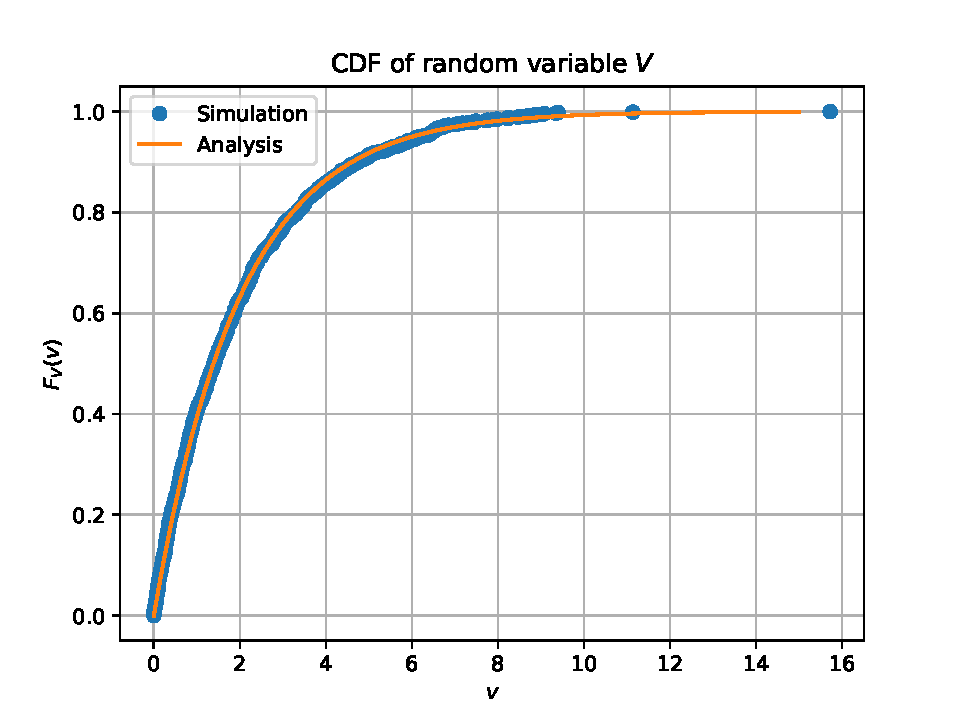
\includegraphics[width=\columnwidth]{/home/chinni/digitalc/figs/V_cdf.pdf}
\caption{The CDF of $V$}
\label{fig:log_uni_cdf}
\end{figure}
\item Find a theoretical expression for $F_V(x)$.
\begin{flalign}
	F_V(x) &= P(V < x)&\\
	&= P(-2\ln\brak{1-U} < x)&\\
	&= P(U < 1 - e^{\frac{-x}{2}})&\\
	&= F_U(1 - e^{\frac{-x}{2}})
\end{flalign}
Using $F_U(x)$ defined in \eqref{eq:uni_cdf},
\begin{align}
	F_V(x) &=
	\begin{cases}
		0 & x < 0\\
		1 - e^{\frac{-x}{2}} & x \ge 0
	\end{cases}
\end{align} 
%
%\item
%Generate the Rayleigh distribution from Uniform. Verify your result through graphical plots.
\end{enumerate}
\section{Triangular Distribution}
\begin{enumerate}[label=\thesection.\arabic*
,ref=\thesection.\theenumi]
%
\item Generate 
	\begin{align}
		T = U_1+U_2
	\end{align}
\\
\solution Download the following files and execute the  C program.
\begin{center}
\fbox{\parbox{10.5cm}{\href{https://github.com/Prathyushakorepu/FWC2/blob/main/Digital-communications/codes/tri/tri.c}{https://github.com/Prathyushakorepu/FWC2/blob/main\\/Digital-communications/codes/tri/tri.c}}}
\end{center}
\item Find the CDF of $T$.\\
\solution Loading the samples from Uni1.dat and Uni2.dat in python, the CDF is plotted in Fig. 5.4.2.1 using the code below
\begin{center}
\fbox{\parbox{10.5cm}{\href{https://github.com/Prathyushakorepu/FWC2/blob/main/Digital-communications/codes/tri/Tcdf.py}{https://github.com/Prathyushakorepu/FWC2/blob/main\\/Digital-communications/codes/tri/Tcdf.py}}}
\end{center}
\begin{figure}[H]
\centering
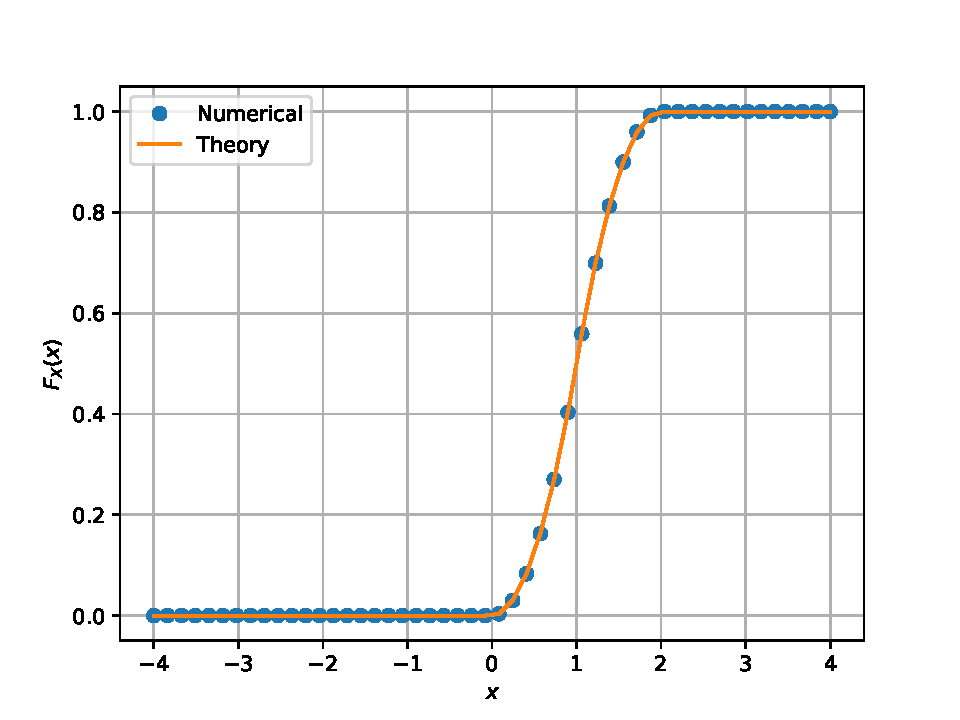
\includegraphics[width=\columnwidth]{/home/chinni/digitalc/figs/T_cdf.pdf}
\caption{The CDF of $T$}
\label{fig:tri_cdf}
\end{figure}
\item Find the PDF of $T$.\\
\solution The PDF of $T$ is plotted in Fig.5.4.3.1 using the code below
\begin{center}
\fbox{\parbox{10.5cm}{\href{https://github.com/Prathyushakorepu/FWC2/blob/main/Digital-communications/codes/tri/TPDF.py}{https://github.com/Prathyushakorepu/FWC2/blob/main\\/Digital-communications/codes/tri/TPDF.py}}}
\end{center}
\begin{figure}[H]
\centering
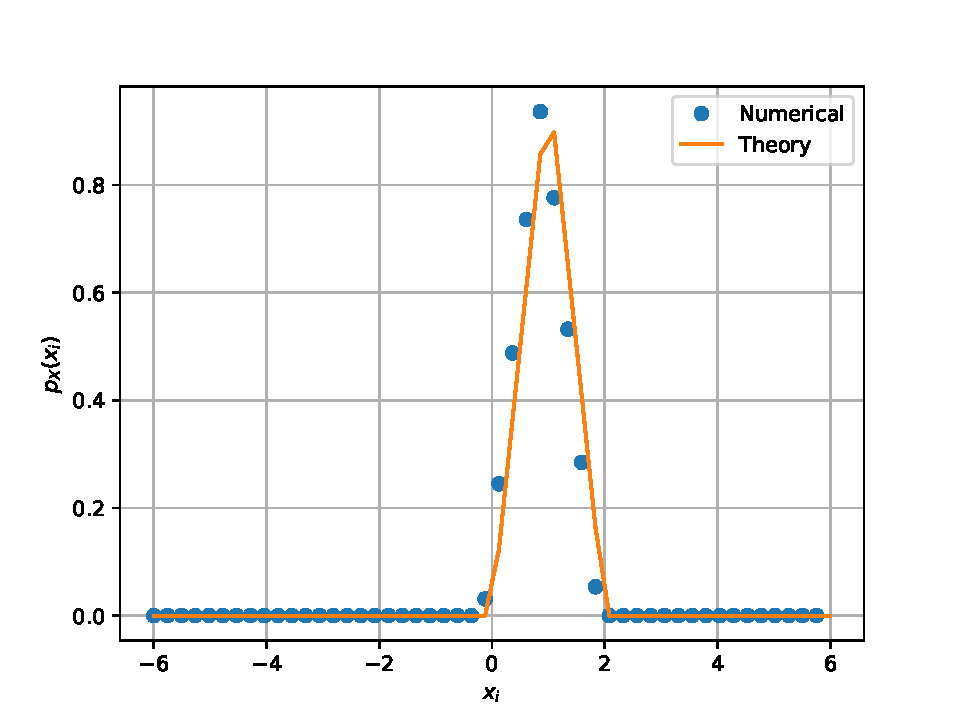
\includegraphics[width=\columnwidth]{/home/chinni/digitalc/figs/T_pdf.pdf}
\caption{The PDF of $T$}
\label{fig:tri_pdf}
\end{figure}
\item Find the theoretical expressions for the PDF and CDF of $T$.\\
\solution Since $T$ is the sum of two independant random variables $U1$ and $U2$, the PDF of $T$ is given by
\begin{flalign}
	p_T(x) &= p_{U1}(x) \ast p_{U2}(x)
\end{flalign}
Using the PDF of $U$ from \eqref{eq:uni_pdf}, the convolution results in
\begin{align}
	p_T(x) &=
	\begin{cases}
		0 & x < 0\\
		x & 0 \le x \le 1\\
		2-x & 1 \le x \le 2\\
		0 & x > 2
	\end{cases}
	\label{eq:tri_pdf}
\end{align}
The CDF of $T$ is found using \eqref{eq:pdf_to_cdf} by replacing $U$ with $T$. Evaluating the integral for the piecewise function $p_T(x)$, 
\begin{align}
	F_T(x) &=
	\begin{cases}
		0 & x < 0\\
		\frac{x^2}{2} & 0 \le x \le 1\\
		2x-\frac{x^2}{2}-1 & 1 \le x \le 2\\
		1 & x > 2
	\end{cases}
\end{align}
\item Verify your results through a plot. \\
\solution The theoretical and numerical plots for the CDF and PDF of $T$ closely match in Fig.5.4.2.1 and Fig.5.4.3.1
\end{enumerate}
\iffalse
\section{Maximum Likelihood}
\begin{enumerate}[label=\thesection.\arabic*
,ref=\thesection.\theenumi]
\item Generate equiprobable $X \in \cbrak{1,-1}$.
\solution hello
\item Generate 
\begin{equation}
Y = AX+N,
\end{equation}
		where $A = 5$ dB,  and $N \sim \gauss{0}{1}$.
	\item Plot $Y$ using a scatter plot.
	\item Guess how to estimate $X$ from $Y$.
\item
\label{ml-ch4_sim}
Find 
\begin{equation}
	P_{e|0} = \pr{\hat{X} = -1|X=1}
\end{equation}
and 
\begin{equation}
	P_{e|1} = \pr{\hat{X} = 1|X=-1}
\end{equation}
%
\item Find $P_e$ assuming that $X$ has equiprobable symbols.
%
\item
Verify by plotting  the theoretical $P_e$ with respect to $A$ from 0 to 10 dB.  
%
\item Now, consider a threshold $\delta$  while estimating $X$ from $Y$. Find the value of $\delta$ that maximizes the theoretical $P_e$.
\item Repeat the above exercise when 
	\begin{align}
		p_{X}(0) = p
	\end{align}
\item Repeat the above exercise using the MAP criterion.
		\end{enumerate}
\section{Gaussian to Other}
\begin{enumerate}[label=\thesection.\arabic*
,ref=\thesection.\theenumi]
\item
Let $X_1 \sim  \gauss{0}{1}$ and $X_2 \sim  \gauss{0}{1}$. Plot the CDF and PDF of
%
\begin{equation}
V = X_1^2 + X_2^2
\end{equation}
%
%
%
\item
If
%
\begin{equation}
F_{V}(x) = 
\begin{cases}
1 - e^{-\alpha x} & x \geq 0 \\
0 & x < 0,
\end{cases}
\end{equation}
%
find $\alpha$.
%
\item
\label{ch3_raleigh_sim}
Plot the CDF and PDf of
%
\begin{equation}
A = \sqrt{V}
\end{equation}
%
\end{enumerate}
\section{Conditional Probability}
\begin{enumerate}[label=\thesection.\arabic*
,ref=\thesection.\theenumi]
\item
\label{ch4_sim}
Plot 
\begin{equation}
P_e = \pr{\hat{X} = -1|X=1}
\end{equation}
%
for 
\begin{equation}
Y = AX+N,
\end{equation}
where $A$ is Raleigh with $E\sbrak{A^2} = \gamma, N \sim \gauss{0}{1}, X \in \brak{-1,1}$ for $0 \le \gamma \le 10$ dB.
%
\item
Assuming that $N$ is a constant, find an expression for $P_e$.  Call this $P_e(N)$
%
\item
%
\label{ch4_anal}
For a function $g$,
\begin{equation}
E\sbrak{g(X)} = \int_{-\infty}^{\infty}g(x)p_{X}(x)\, dx
\end{equation}
%
Find $P_e = E\sbrak{P_e(N)}$.
%
\item
Plot $P_e$ in problems \ref{ch4_sim} and \ref{ch4_anal} on the same graph w.r.t $\gamma$.  Comment.
		\end{enumerate}
\section{Two Dimensions}
Let 
\begin{equation}
\mbf{y} = A\mbf{x} + \mbf{n},
\end{equation}
where 
\begin{align}
x &\in \brak{\mbf{s}_0,\mbf{s}_1}, 
\mbf{s}_0 = 
\begin{pmatrix}
1 
\\
0
\end{pmatrix},
\mbf{s}_1 = 
\begin{pmatrix}
0 
\\
1
\end{pmatrix}
\\
\mbf{n} &= 
\begin{pmatrix}
n_1
\\
n_2
\end{pmatrix},
n_1,n_2 \sim \gauss{0}{1}.
\end{align}
%
\begin{enumerate}[label=\thesection.\arabic*
,ref=\thesection.\theenumi]
%%
\item
\label{ch5_fsk}
Plot 
%
\begin{equation}
\mbf{y}|\mbf{s}_0 \text{ and } \mbf{y}|\mbf{s}_1
\end{equation}
%
on the same graph using a scatter plot.
%
\item
For the above problem, find a decision rule for detecting the symbols $\mbf{s}_0 $ and $\mbf{s}_1$.
%
\item
Plot 
\begin{equation} 
P_e = \pr{\hat{\mbf{x}} = \mbf{s}_1|\mbf{x} = \mbf{s}_0}
\end{equation}
with respect to the SNR from 0 to 10 dB.
%
\item
Obtain an expression for $P_e$. Verify this by comparing the theory and simulation plots on the same graph.
%
		\end{enumerate}
\end{document}
\fi


\chapter{Maximum Likelihood Detection: BPSK}
\iffalse
\let\negmedspace\undefined
\let\negthickspace\undefined
\documentclass[journal,12pt,twocolumn]{IEEEtran}
%\documentclass[conference]{IEEEtran}
%\IEEEoverridecommandlockouts
% The preceding line is only needed to identify funding in the first footnote. If that is unneeded, please comment it out.
\usepackage{cite}
\usepackage{amssymb,amsfonts,amsthm,amsmath}
\usepackage{algorithmic}
\usepackage{graphicx}
\usepackage{textcomp}
\usepackage{xcolor}
\usepackage{txfonts}
\usepackage{listings}
\usepackage{enumitem}
\usepackage{mathtools}
\usepackage{gensymb}

%%
%\usepackage{setspace}
%%\doublespacing
%\singlespacing
%
%%\usepackage{graphicx}
%%\usepackage{amssymb}
%%\usepackage{relsize}
%\usepackage[cmex10]{amsmath}
%%\interdisplaylinepenalty=2500
%%\savesymbol{iint}
%%\usepackage{txfonts}
%%\restoresymbol{TXF}{iint}
%%\usepackage{wasysym}
%\usepackage{amsthm}
%\usepackage{mathrsfs}
%\usepackage{txfonts}
%%\usepackage{stfloats}
%%\usepackage{cite}
%%\usepackage{cases}
%%\usepackage{subfig}
%%\usepackage{xtab}
%%\usepackage{multirow}
%%\usepackage{algorithm}
%%\usepackage{algpseudocode}
%%\usepackage{tikz}
%%\usepackage{circuitikz}
%%\usepackage{verbatim}
\usepackage{hyperref}
%%\usepackage{stmaryrd}
%%\usepackage{tkz-euclide} % loads  TikZ and tkz-base
%%\usetkzobj{all}
    \usepackage{color}                                            %%
    \usepackage{array}                                            %%
    \usepackage{longtable}                                        %%
    \usepackage{calc}                                             %%
    \usepackage{multirow}                                         %%
    \usepackage{hhline}                                           %%
    \usepackage{ifthen}                                           %%
%  %optionally (for landscape tables embedded in another document): %%
%    \usepackage{lscape}     
%%\usepackage{multicol}
%\usepackage{chngcntr}
%\usepackage{enumerate}

%\usepackage{wasysym}
%\newcounter{MYtempeqncnt}
\DeclareMathOperator*{\Res}{Res}
%\renewcommand{\baselinestretch}{2}
\renewcommand\thesection{\arabic{section}}
\renewcommand\thesubsection{\thesection.\arabic{subsection}}
\renewcommand\thesubsubsection{\thesubsection.\arabic{subsubsection}}

\renewcommand\thesectiondis{\arabic{section}}
\renewcommand\thesubsectiondis{\thesectiondis.\arabic{subsection}}
\renewcommand\thesubsubsectiondis{\thesubsectiondis.\arabic{subsubsection}}

% correct bad hyphenation here
\hyphenation{op-tical net-works semi-conduc-tor}
\def\inputGnumericTable{}                                 %%

\lstset{
language=tex,
frame=single, 
breaklines=true
}

\begin{document}
%


\newtheorem{theorem}{Theorem}[section]
\newtheorem{problem}{Problem}
\newtheorem{proposition}{Proposition}[section]
\newtheorem{lemma}{Lemma}[section]
\newtheorem{corollary}[theorem]{Corollary}
\newtheorem{example}{Example}[section]
\newtheorem{definition}[problem]{Definition}
%\newtheorem{thm}{Theorem}[section] 
%\newtheorem{defn}[thm]{Definition}
%\newtheorem{algorithm}{Algorithm}[section]
%\newtheorem{cor}{Corollary}
\newcommand{\BEQA}{\begin{eqnarray}}
\newcommand{\EEQA}{\end{eqnarray}}
\newcommand{\define}{\stackrel{\triangle}{=}}
\bibliographystyle{IEEEtran}
%\bibliographystyle{ieeetr}
\providecommand{\mbf}{\mathbf}
\providecommand{\pr}[1]{\ensuremath{\Pr\left(#1\right)}}
\providecommand{\re}[1]{\ensuremath{\text{Re}\left(#1\right)}}
\providecommand{\im}[1]{\ensuremath{\text{Im}\left(#1\right)}}
\providecommand{\qfunc}[1]{\ensuremath{Q\left(#1\right)}}
\providecommand{\sbrak}[1]{\ensuremath{{}\left[#1\right]}}
\providecommand{\lsbrak}[1]{\ensuremath{{}\left[#1\right.}}
\providecommand{\rsbrak}[1]{\ensuremath{{}\left.#1\right]}}
\providecommand{\brak}[1]{\ensuremath{\left(#1\right)}}
\providecommand{\lbrak}[1]{\ensuremath{\left(#1\right.}}
\providecommand{\rbrak}[1]{\ensuremath{\left.#1\right)}}
\providecommand{\cbrak}[1]{\ensuremath{\left\{#1\right\}}}
\providecommand{\lcbrak}[1]{\ensuremath{\left\{#1\right.}}
\providecommand{\rcbrak}[1]{\ensuremath{\left.#1\right\}}}
\theoremstyle{remark}
\newtheorem{rem}{Remark}
\newcommand{\sgn}{\mathop{\mathrm{sgn}}}
\providecommand{\abs}[1]{\left\vert#1\right\vert}
\providecommand{\res}[1]{\Res\displaylimits_{#1}} 
\providecommand{\norm}[1]{\left\lVert#1\right\rVert}
%\providecommand{\norm}[1]{\lVert#1\rVert}
\providecommand{\mtx}[1]{\mathbf{#1}}
\providecommand{\mean}[1]{E\left[ #1 \right]}
\providecommand{\fourier}{\overset{\mathcal{F}}{ \rightleftharpoons}}
%\providecommand{\hilbert}{\overset{\mathcal{H}}{ \rightleftharpoons}}
\providecommand{\system}{\overset{\mathcal{H}}{ \longleftrightarrow}}
	%\newcommand{\solution}[2]{\textbf{Solution:}{#1}}
\newcommand{\solution}{\noindent \textbf{Solution: }}
\providecommand{\dec}[2]{\ensuremath{\overset{#1}{\underset{#2}{\gtrless}}}}
\newcommand{\myvec}[1]{\ensuremath{\begin{pmatrix}#1\end{pmatrix}}}
\newcommand{\mydet}[1]{\ensuremath{\begin{vmatrix}#1\end{vmatrix}}}
	\newcommand*{\permcomb}[4][0mu]{{{}^{#3}\mkern#1#2_{#4}}}
\newcommand*{\perm}[1][-3mu]{\permcomb[#1]{P}}
\newcommand*{\comb}[1][-1mu]{\permcomb[#1]{C}}
\providecommand{\gauss}[2]{\mathcal{N}\ensuremath{\left(#1,#2\right)}}
%%
%	%\newcommand{\solution}[2]{\textbf{Solution:}{#1}}
%\newcommand{\solution}{\noindent \textbf{Solution: }}
\newcommand{\cosec}{\,\text{cosec}\,}
\newcommand{\sinc}{\,\text{sinc}\,}
\newcommand{\rect}{\,\text{rect}\,}
%\numberwithin{equation}{section}
\numberwithin{equation}{subsection}
%\numberwithin{problem}{section}
%\numberwithin{definition}{section}
\makeatletter
\@addtoreset{figure}{problem}
\makeatother
\let\StandardTheFigure\thefigure
\let\vec\mathbf
\let\j\jmath
%\renewcommand{\thefigure}{\theproblem.\arabic{figure}}
\renewcommand{\thefigure}{\theproblem}
%\setlist[enumerate,1]{before=\renewcommand\theequation{\theenumi.\arabic{equation}}
%\counterwithin{equation}{enumi}
%\renewcommand{\theequation}{\arabic{subsection}.\arabic{equation}}
\def\putbox#1#2#3{\makebox[0in][l]{\makebox[#1][l]{}\raisebox{\baselineskip}[0in][0in]{\raisebox{#2}[0in][0in]{#3}}}}
     \def\rightbox#1{\makebox[0in][r]{#1}}
     \def\centbox#1{\makebox[0in]{#1}}
     \def\topbox#1{\raisebox{-\baselineskip}[0in][0in]{#1}}
     \def\midbox#1{\raisebox{-0.5\baselineskip}[0in][0in]{#1}}
\vspace{3cm}
\title{
%	\logo{
	Probability
%	}
}
%\title{
%	\logo{Matrix Analysis through Octave}{\begin{center}\includegraphics[scale=.24]{tlc}\end{center}}{}{HAMDSP}
%}
% paper title
% can use linebreaks \\ within to get better formatting as desired
%\title{Matrix Analysis through Octave}
%
%
% author names and IEEE memberships
% note positions of commas and nonbreaking spaces ( ~ ) LaTeX will not break
% a structure at a ~ so this keeps an author's name from being broken across
% two lines.
% use \thanks{} to gain access to the first footnote area
% a separate \thanks must be used for each paragraph as LaTeX2e's \thanks
% was not built to handle multiple paragraphs
%
\author{
	G. V. V. Sharma
	%<-this % stops a space
%\thanks{}}
}
% note the % following the last \IEEEmembership and also \thanks - 
% these prevent an unwanted space from occurring between the last author name
% and the end of the author line. i.e., if you had this:
% 
% \author{....lastname \thanks{...} \thanks{...} }
%                     ^------------^------------^----Do not want these spaces!
%
% a space would be appended to the last name and could cause every name on that
% line to be shifted left slightly. This is one of those "LaTeX things". For
% instance, "\textbf{A} \textbf{B}" will typeset as "A B" not "AB". To get
% "AB" then you have to do: "\textbf{A}\textbf{B}"
% \thanks is no different in this regard, so shield the last } of each \thanks
% that ends a line with a % and do not let a space in before the next \thanks.
% Spaces after \IEEEmembership other than the last one are OK (and needed) as
% you are supposed to have spaces between the names. For what it is worth,
% this is a minor point as most people would not even notice if the said evil
% space somehow managed to creep in.
% The paper headers
%\markboth{Journal of \LaTeX\ Class Files,~Vol.~6, No.~1, January~2007}%
%{Shell \MakeLowercase{\textit{et al.}}: Bare Demo of IEEEtran.cls for Journals}
% The only time the second header will appear is for the odd numbered pages
% after the title page when using the twoside option.
% 
% *** Note that you probably will NOT want to include the author's ***
% *** name in the headers of peer review papers.                   ***
% You can use \ifCLASSOPTIONpeerreview for conditional compilation here if
% you desire.
% If you want to put a publisher's ID mark on the page you can do it like
% this:
%\IEEEpubid{0000--0000/00\$00.00~\copyright~2007 IEEE}
% Remember, if you use this you must call \IEEEpubidadjcol in the second
% column for its text to clear the IEEEpubid mark.
% make the title area
\maketitle
\newpage
\tableofcontents
\bigskip
\renewcommand{\thefigure}{\theenumi}
\renewcommand{\thetable}{\theenumi}
%\renewcommand{\theequation}{\theenumi}
%\begin{abstract}
%%\boldmath
%In this letter, an algorithm for evaluating the exact analytical bit error rate  (BER)  for the piecewise linear (PL) combiner for  multiple relays is presented. Previous results were available only for upto three relays. The algorithm is unique in the sense that  the actual mathematical expressions, that are prohibitively large, need not be explicitly obtained. The diversity gain due to multiple relays is shown through plots of the analytical BER, well supported by simulations. 
%
%\end{abstract}
% IEEEtran.cls defaults to using nonbold math in the Abstract.
% This preserves the distinction between vectors and scalars. However,
% if the journal you are submitting to favors bold math in the abstract,
% then you can use LaTeX's standard command \boldmath at the very start
% of the abstract to achieve this. Many IEEE journals frown on math
% in the abstract anyway.
% Note that keywords are not normally used for peerreview papers.
%\begin{IEEEkeywords}
%Cooperative diversity, decode and forward, piecewise linear
%\end{IEEEkeywords}
% For peer review papers, you can put extra information on the cover
% page as needed:
% \ifCLASSOPTIONpeerreview
% \begin{center} \bfseries EDICS Category: 3-BBND \end{center}
% \fi
%
% For peerreview papers, this IEEEtran command inserts a page break and
% creates the second title. It will be ignored for other modes.
%\IEEEpeerreviewmaketitle
%\begin{abstract}
%\end{abstract}
%\iffalse
%% Copyright (C) 2020 Saurabh Joshi
%%% 
%\let\negmedspace\undefined
%\let\negthickspace\undefined
%
%\documentclass[journal,12pt,onecolumn]{IEEEtran}
%%\documentclass[journal,12pt,twocolumn]{IEEEtran}
%%
%\usepackage{setspace}
%\usepackage{gensymb}
%%\doublespacing
%\singlespacing
%
%%\usepackage{graphicx}
%%\usepackage{amssymb}
%%\usepackage{relsize}
%\usepackage[cmex10]{amsmath}
%%\usepackage{amsthm}
%%\interdisplaylinepenalty=2500
%%\savesymbol{iint}
%%\usepackage{txfonts}
%%\restoresymbol{TXF}{iint}
%%\usepackage{wasysym}
%\usepackage{amsthm}
%\usepackage{mathrsfs}
%\usepackage{txfonts}
%\usepackage{stfloats}
%\usepackage{cite}
%\usepackage{cases}
%\usepackage{subfig}
%%\usepackage{xtab}
%\usepackage{longtable}
%\usepackage{multirow}
%%\usepackage{algorithm}
%%\usepackage{algpseudocode}
%\usepackage{enumitem}
%\usepackage{mathtools}
%\usepackage{tikz}
%\usepackage{circuitikz}
%\usepackage{verbatim}
%\usepackage{hyperref}
%%\usepackage{stmaryrd}
%\usepackage{tkz-euclide} % loads  TikZ and tkz-base
%%\usetkzobj{all}
%\usepackage{listings}
%    \usepackage{color}                                            %%
%    \usepackage{array}                                            %%
%    \usepackage{longtable}                                        %%
%    \usepackage{calc}                                             %%
%    \usepackage{multirow}                                         %%
%    \usepackage{hhline}                                           %%
%    \usepackage{ifthen}                                           %%
%  %optionally (for landscape tables embedded in another document): %%
%    \usepackage{lscape}     
%\usepackage{multicol}
%\usepackage{chngcntr}
%\usepackage{iftex}
%%\usepackage[latin9]{inputenc}
%\usepackage{geometry}
%\usepackage{bm}
%%\geometry{verbose,tmargin=2cm,bmargin=3cm,lmargin=1.8cm,rmargin=1.5cm,headheight=2cm,headsep=2cm,footskip=3cm}
%\usepackage{array}
%\newcolumntype{L}[1]{>{\raggedright\let\newline\\\arraybackslash\hspace{0pt}}m{#1}}
%\newcolumntype{C}[1]{>{\centering\let\newline\\\arraybackslash\hspace{0pt}}m{#1}}
%\newcolumntype{R}[1]{>{\raggedleft\let\newline\\\arraybackslash\hspace{0pt}}m{#1}}
%
%%\usepackage{graphicx}
%%\usepackage{setspace}
%%\usepackage{parskip}
%
%\def \hsp {\hspace{3mm}}
%
%\makeatletter
%
%\providecommand{\tabularnewline}{\\}
%
%
%
%\makeatother
%\ifxetex
%\usepackage[T1]{fontenc}
%\usepackage{fontspec}
%%\setmainfont[ Path = fonts/]{Sanskrit_2003.ttf}
%\newfontfamily\nakulafont[Script=Devanagari,AutoFakeBold=2,Path = fonts/]{Nakula}
%%\newfontfamily\liberationfont{Liberation Sans Narrow}
%%\newfontfamily\liberationsansfont{Liberation Sans}
%\fi
%\usepackage{tikz}
%\usepackage{xcolor}
%%\usepackage{enumerate}
%
%%\usepackage{wasysym}
%%\newcounter{MYtempeqncnt}
%\DeclareMathOperator*{\Res}{Res}
%%\renewcommand{\baselinestretch}{2}
%\renewcommand\thesection{\arabic{section}}
%\renewcommand\thesubsection{\thesection.\arabic{subsection}}
%\renewcommand\thesubsubsection{\thesubsection.\arabic{subsubsection}}
%
%\renewcommand\thesectiondis{\arabic{section}}
%\renewcommand\thesubsectiondis{\thesectiondis.\arabic{subsection}}
%\renewcommand\thesubsubsectiondis{\thesubsectiondis.\arabic{subsubsection}}
%
%% correct bad hyphenation here
%\hyphenation{op-tical net-works semi-conduc-tor}
%\def\inputGnumericTable{}                                 %%
%
%\lstset{
%language=tex,
%frame=single, 
%breaklines=true
%}
%
%%\begin{document}
%%
%
%
%\newtheorem{theorem}{Theorem}[section]
%\newtheorem{problem}{Problem}
%\newtheorem{proposition}{Proposition}[section]
%\newtheorem{lemma}{Lemma}[section]
%\newtheorem{corollary}[theorem]{Corollary}
%\newtheorem{example}{Example}[section]
%\newtheorem{definition}[problem]{Definition}
%%\newtheorem{thm}{Theorem}[section] 
%%\newtheorem{defn}[thm]{Definition}
%%\newtheorem{algorithm}{Algorithm}[section]
%%\newtheorem{cor}{Corollary}
%\newcommand{\BEQA}{\begin{eqnarray}}
%\newcommand{\EEQA}{\end{eqnarray}}
%\newcommand{\define}{\stackrel{\triangle}{=}}
%
%\bibliographystyle{IEEEtran}
%%\bibliographystyle{ieeetr}
%
%
%\providecommand{\mbf}{\mathbf}
%\providecommand{\pr}[1]{\ensuremath{\Pr\left(#1\right)}}
%\providecommand{\qfunc}[1]{\ensuremath{Q\left(#1\right)}}
%\providecommand{\sbrak}[1]{\ensuremath{{}\left[#1\right]}}
%\providecommand{\lsbrak}[1]{\ensuremath{{}\left[#1\right.}}
%\providecommand{\rsbrak}[1]{\ensuremath{{}\left.#1\right]}}
%\providecommand{\brak}[1]{\ensuremath{\left(#1\right)}}
%\providecommand{\lbrak}[1]{\ensuremath{\left(#1\right.}}
%\providecommand{\rbrak}[1]{\ensuremath{\left.#1\right)}}
%\providecommand{\cbrak}[1]{\ensuremath{\left\{#1\right\}}}
%\providecommand{\lcbrak}[1]{\ensuremath{\left\{#1\right.}}
%\providecommand{\rcbrak}[1]{\ensuremath{\left.#1\right\}}}
%\theoremstyle{remark}
%\newtheorem{rem}{Remark}
%\newcommand{\sgn}{\mathop{\mathrm{sgn}}}
%\providecommand{\abs}[1]{\left\vert#1\right\vert}
%\providecommand{\res}[1]{\Res\displaylimits_{#1}} 
%\providecommand{\norm}[1]{\left\lVert#1\right\rVert}
%%\providecommand{\norm}[1]{\lVert#1\rVert}
%\providecommand{\mtx}[1]{\mathbf{#1}}
%\providecommand{\mean}[1]{E\left[ #1 \right]}
%%\numberwithin{equation}{section}
%\numberwithin{equation}{section}
%%\numberwithin{problem}{section}
%%\numberwithin{definition}{section}
%\makeatletter
%\@addtoreset{figure}{problem}
%\makeatother
%
%\let\StandardTheFigure\thefigure
%\let\vec\mathbf
%%\renewcommand{\thefigure}{\theproblem.\arabic{figure}}
%\renewcommand{\thefigure}{\theproblem}
%%\setlist[enumerate,1]{before=\renewcommand\theequation{\theenumi.\arabic{equation}}
%%\counterwithin{equation}{enumi}
%
%
%%\renewcommand{\theequation}{\arabic{subsection}.\arabic{equation}}
%
%\vspace{3cm}
%
%
%%\usepackage{babel}
%\begin{document}
%
%\begin{tabular}{L{6cm} C{5cm} R{5cm} }
%
%	\definecolor{circleorange}{rgb}{1,0.17,0.08}
%\definecolor{darkorange}{rgb}{1,0.27,0.1}
%\definecolor{orange2}{rgb}{1,0.5,0.15}
%\definecolor{orange3}{rgb}{1,0.65,0.25}
%\definecolor{yellow1}{rgb}{0.95,0.77,0.2}
%%\begin{tikzpicture}[scale=0.2,every node/.style={transform shape}]
%\begin{tikzpicture}[scale=0.1,every node/.style={transform shape}]
%\draw [fill=circleorange,circleorange] (5,10) circle (1.15); 
%\fill [darkorange] (5.06,8) -- (5.06,2) -- (7.3,1.2) -- (7.3,8.8) -- (5.06,8);
%\fill [darkorange] (4.94,8) -- (4.94,2) -- (2.7,1.2) -- (2.7,8.8) -- (4.94,8);
%\fill [orange2]    (7.4,8.4) -- (7.4,1.6) -- (8.2,1.2) -- (8.2,8.8) -- (7.4,8.4);
%\fill [orange2]    (2.6,8.4) -- (2.6,1.6) -- (1.8,1.2) -- (1.8,8.8) -- (2.6,8.4);
%\fill [orange3]    (8.3,8.4) -- (8.3,1.6) -- (9.0,1.2) -- (9.0,8.8) -- (8.3,8.4);
%\fill [orange3]    (1.7,8.4) -- (1.7,1.6) -- (1.0,1.2) -- (1.0,8.8) -- (1.7,8.4);
%\fill [yellow1]    (9.1,8.4) -- (9.1,1.6) -- (9.7,1.2) -- (9.7,8.8) -- (9.1,8.4);
%\fill [yellow1]    (0.9,8.4) -- (0.9,1.6) -- (0.3,1.2) -- (0.3,8.8) -- (0.9,8.4);
%\ifxetex
%\node [scale=2.1] at (5,-0.1)  {   {\bf {\nakulafont  भारतीय प्रौद्योगिकी संस्थान हैदराबाद }} };
%\node [scale=1.8] at (5,-1.2) {   {\bf { Indian Institute of Technology Hyderabad}} };
%%\node [scale=1.8] at (5,-1.2) {   {\bf {\liberationsansfont Indian Institute of Technology Hyderabad}} };
%\fi
%\end{tikzpicture}
%% \includegraphics[scale=0.05]{logo_iith} \newline
%
%& Assignments 
%	&
%	AI1110
%\end{tabular}
%
%
%\vspace{-6mm}
%\begin{center}
%%\includegraphics[scale=0.95]{Yellow-Line}
%\begin{tikzpicture}
%\definecolor{yellow1}{rgb}{0.95,0.77,0.2}
%\draw[line width=0.75mm, yellow1] (0,0) -- (\textwidth,0);
%\end{tikzpicture}
%\par\end{center}
		\numberwithin{equation}{enumi}
\section{Uniform Random Numbers}
Let $U$ be a uniform random variable between 0 and 1.
\begin{enumerate}[label=\thesection.\arabic*
,ref=\thesection.\theenumi]
\item Generate $10^6$ samples of $U$ using a C program and save into a file called uni.dat .
\\
\solution Download the following files and execute the  C program.
\begin{lstlisting}
codes/exrand.c
codes/coeffs.h
\end{lstlisting}
%
\item
Load the uni.dat file into python and plot the empirical CDF of $U$ using the samples in uni.dat. The CDF is defined as
\begin{align}
F_{U}(x) = \pr{U \le x}
\end{align}
\\
\solution  The following code plots Fig. \ref{fig:uni_cdf}
\begin{lstlisting}
codes/cdf_plot.py
\end{lstlisting}
\begin{figure}
\centering
\includegraphics[width=\columnwidth]{./figs/uni_cdf}
\caption{The CDF of $U$}
\label{fig:uni_cdf}
\end{figure}
%
\item
Find a  theoretical expression for $F_{U}(x)$.
\item
The mean of $U$ is defined as
%
\begin{equation}
E\sbrak{U} = \frac{1}{N}\sum_{i=1}^{N}U_i
\end{equation}
%
and its variance as
%
\begin{equation}
\text{var}\sbrak{U} = E\sbrak{U- E\sbrak{U}}^2 
\end{equation}
Write a C program to  find the mean and variance of $U$. 
\item Verify your result theoretically given that
%
\begin{equation}
E\sbrak{U^k} = \int_{-\infty}^{\infty}x^kdF_{U}(x)
\end{equation}
\end{enumerate}
\section{Central Limit Theorem}
%
\begin{enumerate}[label=\thesection.\arabic*
,ref=\thesection.\theenumi]
%
\item
Generate $10^6$ samples of the random variable
%
\begin{equation}
X = \sum_{i=1}^{12}U_i -6
\end{equation}
%
using a C program, where $U_i, i = 1,2,\dots, 12$ are  a set of independent uniform random variables between 0 and 1
and save in a file called gau.dat
%
\item
Load gau.dat in python and plot the empirical CDF of $X$ using the samples in gau.dat. What properties does a CDF have?
\\
\solution The CDF of $X$ is plotted in Fig. \ref{fig:gauss_cdf}
\begin{figure}
\centering
\includegraphics[width=\columnwidth]{./figs/gauss_cdf}
\caption{The CDF of $X$}
\label{fig:gauss_cdf}
\end{figure}
\item
Load gau.dat in python and plot the empirical PDF of $X$ using the samples in gau.dat. The PDF of $X$ is defined as
\begin{align}
p_{X}(x) = \frac{d}{dx}F_{X}(x)
\end{align}
What properties does the PDF have?
\\
\solution The PDF of $X$ is plotted in Fig. \ref{fig:gauss_pdf} using the code below
\begin{lstlisting}
codes/pdf_plot.py
\end{lstlisting}
\begin{figure}
\centering
\includegraphics[width=\columnwidth]{./figs/gauss_pdf}
\caption{The PDF of $X$}
\label{fig:gauss_pdf}
\end{figure}
\item Find the mean and variance of $X$ by writing a C program.
\item Given that 
\begin{align}
p_{X}(x) = \frac{1}{\sqrt{2\pi}}\exp\brak{-\frac{x^2}{2}}, -\infty < x < \infty,
\end{align}
repeat the above exercise theoretically.
%
\end{enumerate}
\section{From Uniform to Other}
\begin{enumerate}[label=\thesection.\arabic*
,ref=\thesection.\theenumi]
%
\item
Generate samples of 
%
\begin{equation}
V = -2\ln\brak{1-U}
\end{equation}
%
and plot its CDF.  
\item Find a theoretical expression for $F_V(x)$.
%
%\item
%Generate the Rayleigh distribution from Uniform. Verify your result through graphical plots.
\end{enumerate}
\section{Triangular Distribution}
\begin{enumerate}[label=\thesection.\arabic*
,ref=\thesection.\theenumi]
%
\item Generate 
	\begin{align}
		T = U_1+U_2
	\end{align}
\item Find the CDF of $T$.
\item Find the PDF of $T$.
\item Find the theoretical expressions for the PDF and CDF of $T$.
\item Verify your results through a plot. 
\end{enumerate}
		\fi
\section{Maximum Likelihood}
\begin{enumerate}[label=\thesection.\arabic*
,ref=\thesection.\theenumi]
\item Generate equiprobable $X \in \cbrak{1,-1}$.\\
\solution $X$ can be generated in python using the below code section,
\begin{lstlisting}[language=python,frame=single]
import numpy as np	
num_samples = 500
x_var = np.random.binomial(1, 0.5, num_samples)
\end{lstlisting}
\item Generate 
\begin{equation}
Y = AX+N,
\end{equation}
		where $A = 5$ dB,  and $N \sim \gauss{0}{1}$.\\
		\solution $Y$ can be generated in python using the below code section,
\begin{lstlisting}[language=python,frame=single]
import numpy as np	
num_samples = 500
x_var = np.random.binomial(1, 0.5, num_samples)*2-1
n_var = np.random.normal(0, 1, num_samples)
A_db = 5
A = 10**(0.1*A_db)
y_var = A*x_var + n_var
\end{lstlisting}
	\item Plot $Y$ using a scatter plot.\\
	\solution The scatter plot of $Y$ is plotted in Fig.6.1.3.1 using the below code,
\begin{center}
\fbox{\parbox{10.5cm}{\href{https://github.com/Prathyushakorepu/FWC2/blob/main/Digital-communications/codes/ML/bpsk-scatter.py}{https://github.com/Prathyushakorepu/FWC2/blob/main/Digital-communications/codes/ML/bpsk-scatter.py}}}
\end{center}	
\begin{figure}
\centering
\includegraphics[width=\columnwidth]{/home/chinni/digitalc/figs/bpsk_scatter.pdf}
\caption{Scatter plot of $Y$}
\label{fig:bpsk_scatter}
\end{figure}	
%\begin{center}
%\fbox{\parbox{10.5cm}{\href{https://github.com/Prathyushakorepu/FWC2/blob/main/Digital-communications/codes/tri/TPDF.py}{https://github.com/Prathyushakorepu/FWC2/blob/main\\/Digital-communications/codes/tri/TPDF.py}}}
%\end{center}
%\begin{figure}[H]
%\centering
%\includegraphics[width=\columnwidth]{./figs/chapter3/bpsk_scatter.pdf}
%\caption{Scatter plot of $Y$}
%\label{fig:bpsk_scatter}
%\end{figure}
	\item Guess how to estimate $X$ from $Y$.\\
	\solution
\begin{equation}
y \dec{1}{-1} 0
\label{eq:bpsk_decision}
\end{equation}
\item
\label{ml-ch4_sim}
Find 
\begin{equation}
	P_{e|0} = \pr{\hat{X} = -1|X=1}
\end{equation}
and 
\begin{equation}
	P_{e|1} = \pr{\hat{X} = 1|X=-1}
\end{equation}
\\
\solution Based on the decision rule in \eqref{eq:bpsk_decision},
\begin{flalign*}
	\pr{\hat{X} = -1|X=1} &= \pr{Y < 0|X=1}&\\
	&= \pr{AX + N < 0|X=1}&\\ 
	&= \pr{A + N < 0}&\\
	&= \pr{N < -A}
\end{flalign*}
Similarly,
\begin{flalign*}
	\pr{\hat{X} = 1|X=-1} &= \pr{Y > 0|X=-1}&\\
	&= \pr{N > A}
\end{flalign*}
Since $N \sim \gauss{0}{1}$,
\begin{flalign}
	\label{eq:std_norm_symmetric}
	\pr{N < -A} &= \pr{N > A}&\\
	\label{eq:bpks_prob_err_cond}
	\implies P_{e|0} &= P_{e|1} = \pr{N > A}
\end{flalign}
%
\item Find $P_e$ assuming that $X$ has equiprobable symbols.\\
\solution
\begin{flalign}
	P_e &= \pr{X=1}P_{e|1} + \pr{X=-1}P_{e|0}&\\
	\intertext{Since $X$ is equiprobable}\\
	\label{eq:bpsk_prob_error_equi}
	P_e &= \frac{1}{2}P_{e|1} + \frac{1}{2}P_{e|0}
\end{flalign}
Substituting from \eqref{eq:bpks_prob_err_cond}
\begin{equation}
	P_e = \pr{N > A}
\end{equation}
Given a random varible $X \sim \gauss{0}{1}$ the Q-function is defined as
\begin{align}
	Q(x) &= \pr{X > x}\\
	\label{eq:q_func_integral}
	Q(x) &= \frac{1}{\sqrt{2\pi}} \int_x^\infty \exp\left(-\frac{u^2}{2}\right) \, du.\\
\end{align}
Using the Q-function, $P_e$ is rewritten as
\begin{equation}
	P_e = Q(A)
\end{equation} 
%
\item
Verify by plotting  the theoretical $P_e$ with respect to $A$ from 0 to 10 dB. \\
\solution The theoretical $P_e$ is plotted in Fig.6.1.7.1, along with numerical estimations from generated samples of $Y$. The below code is used for the plot, 
\begin{center}
\fbox{\parbox{10.5cm}{\href{https://github.com/Prathyushakorepu/FWC2/blob/main/Digital-communications/codes/ML/bpsk-pe-vs-snr.py}{https://github.com/Prathyushakorepu/FWC2/blob/main/Digital-communications/codes/ML/bpsk-pe-vs-snr.py}}}
\end{center}	
\begin{figure}[H]
\centering
\includegraphics[width=\columnwidth]{/home/chinni/digitalc/figs/bpsk_pe_snr.pdf}
\caption{$P_e$ versus $A$ plot}
\label{fig:bpsk_pe_snr}
\end{figure}
 
%
\item Now, consider a threshold $\delta$  while estimating $X$ from $Y$. Find the value of $\delta$ that maximizes the theoretical $P_e$.\\
\solution Given the decision rule, 
\begin{equation}
y \dec{1}{-1} \delta
\label{eq:bpsk_decision_delta}
\end{equation}
\begin{flalign*}
	P_{e|0} &= \pr{\hat{X} = -1|X=1}&\\
	&= \pr{Y < \delta|X=1}&\\
	&= \pr{AX + N < \delta|X=1}&\\ 
	&= \pr{A + N < \delta}&\\
	&= \pr{N < -A + \delta}&\\
	&= \pr{N > A - \delta}&\\
	&= Q(A-\delta)
\end{flalign*}
\begin{flalign*}
	P_{e|1} &= \pr{\hat{X} = 1|X=-1}&\\
	&= \pr{Y > \delta|X=-1}&\\
	&= \pr{N > A + \delta}&\\
	&= Q(A+\delta)
\end{flalign*}
Using \eqref{eq:bpsk_prob_error_equi}, $P_e$ is given by
\begin{flalign}
	P_e &= \frac{1}{2}Q(A+\delta) + \frac{1}{2}Q(A-\delta)
\end{flalign}
Using the integral for Q-function from \eqref{eq:q_func_integral},
\begin{align}
	\label{eq:prob_error_delta_equi}
	P_e &= k(\int_{A+\delta}^\infty \exp\left(-\frac{u^2}{2}\right) \, du + \int_{A-\delta}^\infty \exp\left(-\frac{u^2}{2}\right) \, du)\\
	\intertext{where k is a constant}	\nonumber
\end{align}
Differentiating (6.1.8.3) wrt $\delta$ (using Leibniz's rule) and equating to $0$, we get
\begin{flalign*}
	\exp\left(-\frac{(A+\delta)^2}{2}\right)-\exp\left(-\frac{(A-\delta)^2}{2}\right) &= 0&\\
	\frac{\exp\left(-\frac{(A+\delta)^2}{2}\right)}{\exp\left(-\frac{(A-\delta)^2}{2}\right)} &= 1&\\
	\exp\left(-\frac{(A+\delta)^2-(A-\delta)^2}{2}\right) &= 1&\\
	\exp\left(-2A\delta\right) &= 1&\\
	\intertext{Taking $\ln$ on both sides}\\
	-2A\delta &= 0&\\
	\implies \delta &= 0
\end{flalign*}
$P_e$ is maximum for $\delta = 0$

\item Repeat the above exercise when 
	\begin{align}
		p_{X}(0) = p
	\end{align}
	\solution Since $X$ is not equiprobable, $P_e$ is given by,
\begin{flalign}
	P_e &= (1-p)P_{e|1} + pP_{e|0}&\\
	&= (1-p)Q(A+\delta) + pQ(A-\delta)
\end{flalign}
Using the integral for Q-function from \eqref{eq:q_func_integral},
\begin{multline}
	\label{eq:prob_error_delta_nonequi}
	P_e = k((1-p)\int_{A+\delta}^\infty \exp\left(-\frac{u^2}{2}\right) \, du + \\
	p\int_{A-\delta}^\infty \exp\left(-\frac{u^2}{2}\right) \, du)
\end{multline}
where $k$ is a constant.\\
Following the same steps as in problem 6.1.8, $\delta$ for maximum $P_e$ evaluates to,
\begin{equation}
	\delta = \frac{1}{2A}\ln\left(\frac{1}{p}-1\right)
\end{equation}
\item Repeat the above exercise using the MAP criterion.\\
\solution 
The MAP rule can be stated as\\
\begin{flalign}
\label{eq:map_rule}
\text{Set } \hat{x} &= x_i \text{ if}&\\ \nonumber
p_X(x_k)p_Y(y|x_k) &\text{ is maximum for } k = i
\end{flalign}
For the case of BPSK, the point of equality between $p_X(x=1)p_Y(y|x=1)$ and $p_X(x=-1)p_Y(y|x=-1)$ is the optimum threshold. If this threshold is $\delta$, then
\begin{flalign*}
	pp_Y(y|x=1) > (1-p)p_Y(y|x=-1) &\text{ when } y > \delta&\\
	pp_Y(y|x=1) < (1-p)p_Y(y|x=-1) &\text{ when } y < \delta 	
\end{flalign*}
The above inequalities can be visualized in Fig.6.1.10.1 for $p = 0.3$ and $A = 3$.
\begin{figure}[H]
\centering
\includegraphics[width=\columnwidth]{/home/chinni/digitalc/figs/bpsk_map_density.pdf}
\caption{$p_X(X=x_i)p_Y(y|x=x_i)$ versus $y$ plot for $X \in \{-1,1\}$}
\label{fig:bpsk_map_density}
\end{figure}
Given $Y=AX+N$ where $N \sim \gauss{0}{1}$, the optimum threshold is found as solution to the below equation
\begin{equation}
	p\exp\left(-\frac{(y_{eq}-A)^2}{2}\right) = (1-p)\exp\left(-\frac{(y_{eq}+A)^2}{2}\right)
\end{equation}
Solving for $y_{eq}$, we get
\begin{equation}
	y_{eq} = \delta = \frac{1}{2A}\ln\left(\frac{1}{p}-1\right)
\end{equation}
which is same as $\delta$ obtained in problem 6.1.9


		\end{enumerate}
		\iffalse
\section{Gaussian to Other}
\begin{enumerate}[label=\thesection.\arabic*
,ref=\thesection.\theenumi]
\item
Let $X_1 \sim  \gauss{0}{1}$ and $X_2 \sim  \gauss{0}{1}$. Plot the CDF and PDF of
%
\begin{equation}
V = X_1^2 + X_2^2
\end{equation}
%
%
%
\item
If
%
\begin{equation}
F_{V}(x) = 
\begin{cases}
1 - e^{-\alpha x} & x \geq 0 \\
0 & x < 0,
\end{cases}
\end{equation}
%
find $\alpha$.
%
\item
\label{ch3_raleigh_sim}
Plot the CDF and PDf of
%
\begin{equation}
A = \sqrt{V}
\end{equation}
%
\end{enumerate}
\section{Conditional Probability}
\begin{enumerate}[label=\thesection.\arabic*
,ref=\thesection.\theenumi]
\item
\label{ch4_sim}
Plot 
\begin{equation}
P_e = \pr{\hat{X} = -1|X=1}
\end{equation}
%
for 
\begin{equation}
Y = AX+N,
\end{equation}
where $A$ is Raleigh with $E\sbrak{A^2} = \gamma, N \sim \gauss{0}{1}, X \in \brak{-1,1}$ for $0 \le \gamma \le 10$ dB.
%
\item
Assuming that $N$ is a constant, find an expression for $P_e$.  Call this $P_e(N)$
%
\item
%
\label{ch4_anal}
For a function $g$,
\begin{equation}
E\sbrak{g(X)} = \int_{-\infty}^{\infty}g(x)p_{X}(x)\, dx
\end{equation}
%
Find $P_e = E\sbrak{P_e(N)}$.
%
\item
Plot $P_e$ in problems \ref{ch4_sim} and \ref{ch4_anal} on the same graph w.r.t $\gamma$.  Comment.
		\end{enumerate}
\section{Two Dimensions}
Let 
\begin{equation}
\mbf{y} = A\mbf{x} + \mbf{n},
\end{equation}
where 
\begin{align}
x &\in \brak{\mbf{s}_0,\mbf{s}_1}, 
\mbf{s}_0 = 
\begin{pmatrix}
1 
\\
0
\end{pmatrix},
\mbf{s}_1 = 
\begin{pmatrix}
0 
\\
1
\end{pmatrix}
\\
\mbf{n} &= 
\begin{pmatrix}
n_1
\\
n_2
\end{pmatrix},
n_1,n_2 \sim \gauss{0}{1}.
\end{align}
%
\begin{enumerate}[label=\thesection.\arabic*
,ref=\thesection.\theenumi]
%%
\item
\label{ch5_fsk}
Plot 
%
\begin{equation}
\mbf{y}|\mbf{s}_0 \text{ and } \mbf{y}|\mbf{s}_1
\end{equation}
%
on the same graph using a scatter plot.
%
\item
For the above problem, find a decision rule for detecting the symbols $\mbf{s}_0 $ and $\mbf{s}_1$.
%
\item
Plot 
\begin{equation} 
P_e = \pr{\hat{\mbf{x}} = \mbf{s}_1|\mbf{x} = \mbf{s}_0}
\end{equation}
with respect to the SNR from 0 to 10 dB.
%
\item
Obtain an expression for $P_e$. Verify this by comparing the theory and simulation plots on the same graph.
%
		\end{enumerate}
\end{document}
\fi


\chapter{Transformation of Random Variables}
\iffalse
\let\negmedspace\undefined
\let\negthickspace\undefined
\documentclass[journal,12pt,twocolumn]{IEEEtran}
%\documentclass[conference]{IEEEtran}
%\IEEEoverridecommandlockouts
% The preceding line is only needed to identify funding in the first footnote. If that is unneeded, please comment it out.
\usepackage{cite}
\usepackage{amssymb,amsfonts,amsthm,amsmath}
\usepackage{algorithmic}
\usepackage{graphicx}
\usepackage{textcomp}
\usepackage{xcolor}
\usepackage{txfonts}
\usepackage{listings}
\usepackage{enumitem}
\usepackage{mathtools}
\usepackage{gensymb}

%%
%\usepackage{setspace}
%%\doublespacing
%\singlespacing
%
%%\usepackage{graphicx}
%%\usepackage{amssymb}
%%\usepackage{relsize}
%\usepackage[cmex10]{amsmath}
%%\interdisplaylinepenalty=2500
%%\savesymbol{iint}
%%\usepackage{txfonts}
%%\restoresymbol{TXF}{iint}
%%\usepackage{wasysym}
%\usepackage{amsthm}
%\usepackage{mathrsfs}
%\usepackage{txfonts}
%%\usepackage{stfloats}
%%\usepackage{cite}
%%\usepackage{cases}
%%\usepackage{subfig}
%%\usepackage{xtab}
%%\usepackage{multirow}
%%\usepackage{algorithm}
%%\usepackage{algpseudocode}
%%\usepackage{tikz}
%%\usepackage{circuitikz}
%%\usepackage{verbatim}
\usepackage{hyperref}
%%\usepackage{stmaryrd}
%%\usepackage{tkz-euclide} % loads  TikZ and tkz-base
%%\usetkzobj{all}
    \usepackage{color}                                            %%
    \usepackage{array}                                            %%
    \usepackage{longtable}                                        %%
    \usepackage{calc}                                             %%
    \usepackage{multirow}                                         %%
    \usepackage{hhline}                                           %%
    \usepackage{ifthen}                                           %%
%  %optionally (for landscape tables embedded in another document): %%
%    \usepackage{lscape}     
%%\usepackage{multicol}
%\usepackage{chngcntr}
%\usepackage{enumerate}

%\usepackage{wasysym}
%\newcounter{MYtempeqncnt}
\DeclareMathOperator*{\Res}{Res}
%\renewcommand{\baselinestretch}{2}
\renewcommand\thesection{\arabic{section}}
\renewcommand\thesubsection{\thesection.\arabic{subsection}}
\renewcommand\thesubsubsection{\thesubsection.\arabic{subsubsection}}

\renewcommand\thesectiondis{\arabic{section}}
\renewcommand\thesubsectiondis{\thesectiondis.\arabic{subsection}}
\renewcommand\thesubsubsectiondis{\thesubsectiondis.\arabic{subsubsection}}

% correct bad hyphenation here
\hyphenation{op-tical net-works semi-conduc-tor}
\def\inputGnumericTable{}                                 %%

\lstset{
language=tex,
frame=single, 
breaklines=true
}

\begin{document}
%


\newtheorem{theorem}{Theorem}[section]
\newtheorem{problem}{Problem}
\newtheorem{proposition}{Proposition}[section]
\newtheorem{lemma}{Lemma}[section]
\newtheorem{corollary}[theorem]{Corollary}
\newtheorem{example}{Example}[section]
\newtheorem{definition}[problem]{Definition}
%\newtheorem{thm}{Theorem}[section] 
%\newtheorem{defn}[thm]{Definition}
%\newtheorem{algorithm}{Algorithm}[section]
%\newtheorem{cor}{Corollary}
\newcommand{\BEQA}{\begin{eqnarray}}
\newcommand{\EEQA}{\end{eqnarray}}
\newcommand{\define}{\stackrel{\triangle}{=}}
\bibliographystyle{IEEEtran}
%\bibliographystyle{ieeetr}
\providecommand{\mbf}{\mathbf}
\providecommand{\pr}[1]{\ensuremath{\Pr\left(#1\right)}}
\providecommand{\re}[1]{\ensuremath{\text{Re}\left(#1\right)}}
\providecommand{\im}[1]{\ensuremath{\text{Im}\left(#1\right)}}
\providecommand{\qfunc}[1]{\ensuremath{Q\left(#1\right)}}
\providecommand{\sbrak}[1]{\ensuremath{{}\left[#1\right]}}
\providecommand{\lsbrak}[1]{\ensuremath{{}\left[#1\right.}}
\providecommand{\rsbrak}[1]{\ensuremath{{}\left.#1\right]}}
\providecommand{\brak}[1]{\ensuremath{\left(#1\right)}}
\providecommand{\lbrak}[1]{\ensuremath{\left(#1\right.}}
\providecommand{\rbrak}[1]{\ensuremath{\left.#1\right)}}
\providecommand{\cbrak}[1]{\ensuremath{\left\{#1\right\}}}
\providecommand{\lcbrak}[1]{\ensuremath{\left\{#1\right.}}
\providecommand{\rcbrak}[1]{\ensuremath{\left.#1\right\}}}
\theoremstyle{remark}
\newtheorem{rem}{Remark}
\newcommand{\sgn}{\mathop{\mathrm{sgn}}}
\providecommand{\abs}[1]{\left\vert#1\right\vert}
\providecommand{\res}[1]{\Res\displaylimits_{#1}} 
\providecommand{\norm}[1]{\left\lVert#1\right\rVert}
%\providecommand{\norm}[1]{\lVert#1\rVert}
\providecommand{\mtx}[1]{\mathbf{#1}}
\providecommand{\mean}[1]{E\left[ #1 \right]}
\providecommand{\fourier}{\overset{\mathcal{F}}{ \rightleftharpoons}}
%\providecommand{\hilbert}{\overset{\mathcal{H}}{ \rightleftharpoons}}
\providecommand{\system}{\overset{\mathcal{H}}{ \longleftrightarrow}}
	%\newcommand{\solution}[2]{\textbf{Solution:}{#1}}
\newcommand{\solution}{\noindent \textbf{Solution: }}
\providecommand{\dec}[2]{\ensuremath{\overset{#1}{\underset{#2}{\gtrless}}}}
\newcommand{\myvec}[1]{\ensuremath{\begin{pmatrix}#1\end{pmatrix}}}
\newcommand{\mydet}[1]{\ensuremath{\begin{vmatrix}#1\end{vmatrix}}}
	\newcommand*{\permcomb}[4][0mu]{{{}^{#3}\mkern#1#2_{#4}}}
\newcommand*{\perm}[1][-3mu]{\permcomb[#1]{P}}
\newcommand*{\comb}[1][-1mu]{\permcomb[#1]{C}}
\providecommand{\gauss}[2]{\mathcal{N}\ensuremath{\left(#1,#2\right)}}
%%
%	%\newcommand{\solution}[2]{\textbf{Solution:}{#1}}
%\newcommand{\solution}{\noindent \textbf{Solution: }}
\newcommand{\cosec}{\,\text{cosec}\,}
\newcommand{\sinc}{\,\text{sinc}\,}
\newcommand{\rect}{\,\text{rect}\,}
%\numberwithin{equation}{section}
\numberwithin{equation}{subsection}
%\numberwithin{problem}{section}
%\numberwithin{definition}{section}
\makeatletter
\@addtoreset{figure}{problem}
\makeatother
\let\StandardTheFigure\thefigure
\let\vec\mathbf
\let\j\jmath
%\renewcommand{\thefigure}{\theproblem.\arabic{figure}}
\renewcommand{\thefigure}{\theproblem}
%\setlist[enumerate,1]{before=\renewcommand\theequation{\theenumi.\arabic{equation}}
%\counterwithin{equation}{enumi}
%\renewcommand{\theequation}{\arabic{subsection}.\arabic{equation}}
\def\putbox#1#2#3{\makebox[0in][l]{\makebox[#1][l]{}\raisebox{\baselineskip}[0in][0in]{\raisebox{#2}[0in][0in]{#3}}}}
     \def\rightbox#1{\makebox[0in][r]{#1}}
     \def\centbox#1{\makebox[0in]{#1}}
     \def\topbox#1{\raisebox{-\baselineskip}[0in][0in]{#1}}
     \def\midbox#1{\raisebox{-0.5\baselineskip}[0in][0in]{#1}}
\vspace{3cm}
\title{
%	\logo{
	Probability
%	}
}
%\title{
%	\logo{Matrix Analysis through Octave}{\begin{center}\includegraphics[scale=.24]{tlc}\end{center}}{}{HAMDSP}
%}
% paper title
% can use linebreaks \\ within to get better formatting as desired
%\title{Matrix Analysis through Octave}
%
%
% author names and IEEE memberships
% note positions of commas and nonbreaking spaces ( ~ ) LaTeX will not break
% a structure at a ~ so this keeps an author's name from being broken across
% two lines.
% use \thanks{} to gain access to the first footnote area
% a separate \thanks must be used for each paragraph as LaTeX2e's \thanks
% was not built to handle multiple paragraphs
%
\author{
	G. V. V. Sharma
	%<-this % stops a space
%\thanks{}}
}
% note the % following the last \IEEEmembership and also \thanks - 
% these prevent an unwanted space from occurring between the last author name
% and the end of the author line. i.e., if you had this:
% 
% \author{....lastname \thanks{...} \thanks{...} }
%                     ^------------^------------^----Do not want these spaces!
%
% a space would be appended to the last name and could cause every name on that
% line to be shifted left slightly. This is one of those "LaTeX things". For
% instance, "\textbf{A} \textbf{B}" will typeset as "A B" not "AB". To get
% "AB" then you have to do: "\textbf{A}\textbf{B}"
% \thanks is no different in this regard, so shield the last } of each \thanks
% that ends a line with a % and do not let a space in before the next \thanks.
% Spaces after \IEEEmembership other than the last one are OK (and needed) as
% you are supposed to have spaces between the names. For what it is worth,
% this is a minor point as most people would not even notice if the said evil
% space somehow managed to creep in.
% The paper headers
%\markboth{Journal of \LaTeX\ Class Files,~Vol.~6, No.~1, January~2007}%
%{Shell \MakeLowercase{\textit{et al.}}: Bare Demo of IEEEtran.cls for Journals}
% The only time the second header will appear is for the odd numbered pages
% after the title page when using the twoside option.
% 
% *** Note that you probably will NOT want to include the author's ***
% *** name in the headers of peer review papers.                   ***
% You can use \ifCLASSOPTIONpeerreview for conditional compilation here if
% you desire.
% If you want to put a publisher's ID mark on the page you can do it like
% this:
%\IEEEpubid{0000--0000/00\$00.00~\copyright~2007 IEEE}
% Remember, if you use this you must call \IEEEpubidadjcol in the second
% column for its text to clear the IEEEpubid mark.
% make the title area
\maketitle
\newpage
\tableofcontents
\bigskip
\renewcommand{\thefigure}{\theenumi}
\renewcommand{\thetable}{\theenumi}
%\renewcommand{\theequation}{\theenumi}
%\begin{abstract}
%%\boldmath
%In this letter, an algorithm for evaluating the exact analytical bit error rate  (BER)  for the piecewise linear (PL) combiner for  multiple relays is presented. Previous results were available only for upto three relays. The algorithm is unique in the sense that  the actual mathematical expressions, that are prohibitively large, need not be explicitly obtained. The diversity gain due to multiple relays is shown through plots of the analytical BER, well supported by simulations. 
%
%\end{abstract}
% IEEEtran.cls defaults to using nonbold math in the Abstract.
% This preserves the distinction between vectors and scalars. However,
% if the journal you are submitting to favors bold math in the abstract,
% then you can use LaTeX's standard command \boldmath at the very start
% of the abstract to achieve this. Many IEEE journals frown on math
% in the abstract anyway.
% Note that keywords are not normally used for peerreview papers.
%\begin{IEEEkeywords}
%Cooperative diversity, decode and forward, piecewise linear
%\end{IEEEkeywords}
% For peer review papers, you can put extra information on the cover
% page as needed:
% \ifCLASSOPTIONpeerreview
% \begin{center} \bfseries EDICS Category: 3-BBND \end{center}
% \fi
%
% For peerreview papers, this IEEEtran command inserts a page break and
% creates the second title. It will be ignored for other modes.
%\IEEEpeerreviewmaketitle
%\begin{abstract}
%\end{abstract}
%\iffalse
%% Copyright (C) 2020 Saurabh Joshi
%%% 
%\let\negmedspace\undefined
%\let\negthickspace\undefined
%
%\documentclass[journal,12pt,onecolumn]{IEEEtran}
%%\documentclass[journal,12pt,twocolumn]{IEEEtran}
%%
%\usepackage{setspace}
%\usepackage{gensymb}
%%\doublespacing
%\singlespacing
%
%%\usepackage{graphicx}
%%\usepackage{amssymb}
%%\usepackage{relsize}
%\usepackage[cmex10]{amsmath}
%%\usepackage{amsthm}
%%\interdisplaylinepenalty=2500
%%\savesymbol{iint}
%%\usepackage{txfonts}
%%\restoresymbol{TXF}{iint}
%%\usepackage{wasysym}
%\usepackage{amsthm}
%\usepackage{mathrsfs}
%\usepackage{txfonts}
%\usepackage{stfloats}
%\usepackage{cite}
%\usepackage{cases}
%\usepackage{subfig}
%%\usepackage{xtab}
%\usepackage{longtable}
%\usepackage{multirow}
%%\usepackage{algorithm}
%%\usepackage{algpseudocode}
%\usepackage{enumitem}
%\usepackage{mathtools}
%\usepackage{tikz}
%\usepackage{circuitikz}
%\usepackage{verbatim}
%\usepackage{hyperref}
%%\usepackage{stmaryrd}
%\usepackage{tkz-euclide} % loads  TikZ and tkz-base
%%\usetkzobj{all}
%\usepackage{listings}
%    \usepackage{color}                                            %%
%    \usepackage{array}                                            %%
%    \usepackage{longtable}                                        %%
%    \usepackage{calc}                                             %%
%    \usepackage{multirow}                                         %%
%    \usepackage{hhline}                                           %%
%    \usepackage{ifthen}                                           %%
%  %optionally (for landscape tables embedded in another document): %%
%    \usepackage{lscape}     
%\usepackage{multicol}
%\usepackage{chngcntr}
%\usepackage{iftex}
%%\usepackage[latin9]{inputenc}
%\usepackage{geometry}
%\usepackage{bm}
%%\geometry{verbose,tmargin=2cm,bmargin=3cm,lmargin=1.8cm,rmargin=1.5cm,headheight=2cm,headsep=2cm,footskip=3cm}
%\usepackage{array}
%\newcolumntype{L}[1]{>{\raggedright\let\newline\\\arraybackslash\hspace{0pt}}m{#1}}
%\newcolumntype{C}[1]{>{\centering\let\newline\\\arraybackslash\hspace{0pt}}m{#1}}
%\newcolumntype{R}[1]{>{\raggedleft\let\newline\\\arraybackslash\hspace{0pt}}m{#1}}
%
%%\usepackage{graphicx}
%%\usepackage{setspace}
%%\usepackage{parskip}
%
%\def \hsp {\hspace{3mm}}
%
%\makeatletter
%
%\providecommand{\tabularnewline}{\\}
%
%
%
%\makeatother
%\ifxetex
%\usepackage[T1]{fontenc}
%\usepackage{fontspec}
%%\setmainfont[ Path = fonts/]{Sanskrit_2003.ttf}
%\newfontfamily\nakulafont[Script=Devanagari,AutoFakeBold=2,Path = fonts/]{Nakula}
%%\newfontfamily\liberationfont{Liberation Sans Narrow}
%%\newfontfamily\liberationsansfont{Liberation Sans}
%\fi
%\usepackage{tikz}
%\usepackage{xcolor}
%%\usepackage{enumerate}
%
%%\usepackage{wasysym}
%%\newcounter{MYtempeqncnt}
%\DeclareMathOperator*{\Res}{Res}
%%\renewcommand{\baselinestretch}{2}
%\renewcommand\thesection{\arabic{section}}
%\renewcommand\thesubsection{\thesection.\arabic{subsection}}
%\renewcommand\thesubsubsection{\thesubsection.\arabic{subsubsection}}
%
%\renewcommand\thesectiondis{\arabic{section}}
%\renewcommand\thesubsectiondis{\thesectiondis.\arabic{subsection}}
%\renewcommand\thesubsubsectiondis{\thesubsectiondis.\arabic{subsubsection}}
%
%% correct bad hyphenation here
%\hyphenation{op-tical net-works semi-conduc-tor}
%\def\inputGnumericTable{}                                 %%
%
%\lstset{
%language=tex,
%frame=single, 
%breaklines=true
%}
%
%%\begin{document}
%%
%
%
%\newtheorem{theorem}{Theorem}[section]
%\newtheorem{problem}{Problem}
%\newtheorem{proposition}{Proposition}[section]
%\newtheorem{lemma}{Lemma}[section]
%\newtheorem{corollary}[theorem]{Corollary}
%\newtheorem{example}{Example}[section]
%\newtheorem{definition}[problem]{Definition}
%%\newtheorem{thm}{Theorem}[section] 
%%\newtheorem{defn}[thm]{Definition}
%%\newtheorem{algorithm}{Algorithm}[section]
%%\newtheorem{cor}{Corollary}
%\newcommand{\BEQA}{\begin{eqnarray}}
%\newcommand{\EEQA}{\end{eqnarray}}
%\newcommand{\define}{\stackrel{\triangle}{=}}
%
%\bibliographystyle{IEEEtran}
%%\bibliographystyle{ieeetr}
%
%
%\providecommand{\mbf}{\mathbf}
%\providecommand{\pr}[1]{\ensuremath{\Pr\left(#1\right)}}
%\providecommand{\qfunc}[1]{\ensuremath{Q\left(#1\right)}}
%\providecommand{\sbrak}[1]{\ensuremath{{}\left[#1\right]}}
%\providecommand{\lsbrak}[1]{\ensuremath{{}\left[#1\right.}}
%\providecommand{\rsbrak}[1]{\ensuremath{{}\left.#1\right]}}
%\providecommand{\brak}[1]{\ensuremath{\left(#1\right)}}
%\providecommand{\lbrak}[1]{\ensuremath{\left(#1\right.}}
%\providecommand{\rbrak}[1]{\ensuremath{\left.#1\right)}}
%\providecommand{\cbrak}[1]{\ensuremath{\left\{#1\right\}}}
%\providecommand{\lcbrak}[1]{\ensuremath{\left\{#1\right.}}
%\providecommand{\rcbrak}[1]{\ensuremath{\left.#1\right\}}}
%\theoremstyle{remark}
%\newtheorem{rem}{Remark}
%\newcommand{\sgn}{\mathop{\mathrm{sgn}}}
%\providecommand{\abs}[1]{\left\vert#1\right\vert}
%\providecommand{\res}[1]{\Res\displaylimits_{#1}} 
%\providecommand{\norm}[1]{\left\lVert#1\right\rVert}
%%\providecommand{\norm}[1]{\lVert#1\rVert}
%\providecommand{\mtx}[1]{\mathbf{#1}}
%\providecommand{\mean}[1]{E\left[ #1 \right]}
%%\numberwithin{equation}{section}
%\numberwithin{equation}{section}
%%\numberwithin{problem}{section}
%%\numberwithin{definition}{section}
%\makeatletter
%\@addtoreset{figure}{problem}
%\makeatother
%
%\let\StandardTheFigure\thefigure
%\let\vec\mathbf
%%\renewcommand{\thefigure}{\theproblem.\arabic{figure}}
%\renewcommand{\thefigure}{\theproblem}
%%\setlist[enumerate,1]{before=\renewcommand\theequation{\theenumi.\arabic{equation}}
%%\counterwithin{equation}{enumi}
%
%
%%\renewcommand{\theequation}{\arabic{subsection}.\arabic{equation}}
%
%\vspace{3cm}
%
%
%%\usepackage{babel}
%\begin{document}
%
%\begin{tabular}{L{6cm} C{5cm} R{5cm} }
%
%	\definecolor{circleorange}{rgb}{1,0.17,0.08}
%\definecolor{darkorange}{rgb}{1,0.27,0.1}
%\definecolor{orange2}{rgb}{1,0.5,0.15}
%\definecolor{orange3}{rgb}{1,0.65,0.25}
%\definecolor{yellow1}{rgb}{0.95,0.77,0.2}
%%\begin{tikzpicture}[scale=0.2,every node/.style={transform shape}]
%\begin{tikzpicture}[scale=0.1,every node/.style={transform shape}]
%\draw [fill=circleorange,circleorange] (5,10) circle (1.15); 
%\fill [darkorange] (5.06,8) -- (5.06,2) -- (7.3,1.2) -- (7.3,8.8) -- (5.06,8);
%\fill [darkorange] (4.94,8) -- (4.94,2) -- (2.7,1.2) -- (2.7,8.8) -- (4.94,8);
%\fill [orange2]    (7.4,8.4) -- (7.4,1.6) -- (8.2,1.2) -- (8.2,8.8) -- (7.4,8.4);
%\fill [orange2]    (2.6,8.4) -- (2.6,1.6) -- (1.8,1.2) -- (1.8,8.8) -- (2.6,8.4);
%\fill [orange3]    (8.3,8.4) -- (8.3,1.6) -- (9.0,1.2) -- (9.0,8.8) -- (8.3,8.4);
%\fill [orange3]    (1.7,8.4) -- (1.7,1.6) -- (1.0,1.2) -- (1.0,8.8) -- (1.7,8.4);
%\fill [yellow1]    (9.1,8.4) -- (9.1,1.6) -- (9.7,1.2) -- (9.7,8.8) -- (9.1,8.4);
%\fill [yellow1]    (0.9,8.4) -- (0.9,1.6) -- (0.3,1.2) -- (0.3,8.8) -- (0.9,8.4);
%\ifxetex
%\node [scale=2.1] at (5,-0.1)  {   {\bf {\nakulafont  भारतीय प्रौद्योगिकी संस्थान हैदराबाद }} };
%\node [scale=1.8] at (5,-1.2) {   {\bf { Indian Institute of Technology Hyderabad}} };
%%\node [scale=1.8] at (5,-1.2) {   {\bf {\liberationsansfont Indian Institute of Technology Hyderabad}} };
%\fi
%\end{tikzpicture}
%% \includegraphics[scale=0.05]{logo_iith} \newline
%
%& Assignments 
%	&
%	AI1110
%\end{tabular}
%
%
%\vspace{-6mm}
%\begin{center}
%%\includegraphics[scale=0.95]{Yellow-Line}
%\begin{tikzpicture}
%\definecolor{yellow1}{rgb}{0.95,0.77,0.2}
%\draw[line width=0.75mm, yellow1] (0,0) -- (\textwidth,0);
%\end{tikzpicture}
%\par\end{center}
		\numberwithin{equation}{enumi}
\section{Uniform Random Numbers}
Let $U$ be a uniform random variable between 0 and 1.
\begin{enumerate}[label=\thesection.\arabic*
,ref=\thesection.\theenumi]
\item Generate $10^6$ samples of $U$ using a C program and save into a file called uni.dat .
\\
\solution Download the following files and execute the  C program.
\begin{lstlisting}
codes/exrand.c
codes/coeffs.h
\end{lstlisting}
%
\item
Load the uni.dat file into python and plot the empirical CDF of $U$ using the samples in uni.dat. The CDF is defined as
\begin{align}
F_{U}(x) = \pr{U \le x}
\end{align}
\\
\solution  The following code plots Fig. \ref{fig:uni_cdf}
\begin{lstlisting}
codes/cdf_plot.py
\end{lstlisting}
\begin{figure}
\centering
\includegraphics[width=\columnwidth]{./figs/uni_cdf}
\caption{The CDF of $U$}
\label{fig:uni_cdf}
\end{figure}
%
\item
Find a  theoretical expression for $F_{U}(x)$.
\item
The mean of $U$ is defined as
%
\begin{equation}
E\sbrak{U} = \frac{1}{N}\sum_{i=1}^{N}U_i
\end{equation}
%
and its variance as
%
\begin{equation}
\text{var}\sbrak{U} = E\sbrak{U- E\sbrak{U}}^2 
\end{equation}
Write a C program to  find the mean and variance of $U$. 
\item Verify your result theoretically given that
%
\begin{equation}
E\sbrak{U^k} = \int_{-\infty}^{\infty}x^kdF_{U}(x)
\end{equation}
\end{enumerate}
\section{Central Limit Theorem}
%
\begin{enumerate}[label=\thesection.\arabic*
,ref=\thesection.\theenumi]
%
\item
Generate $10^6$ samples of the random variable
%
\begin{equation}
X = \sum_{i=1}^{12}U_i -6
\end{equation}
%
using a C program, where $U_i, i = 1,2,\dots, 12$ are  a set of independent uniform random variables between 0 and 1
and save in a file called gau.dat
%
\item
Load gau.dat in python and plot the empirical CDF of $X$ using the samples in gau.dat. What properties does a CDF have?
\\
\solution The CDF of $X$ is plotted in Fig. \ref{fig:gauss_cdf}
\begin{figure}
\centering
\includegraphics[width=\columnwidth]{./figs/gauss_cdf}
\caption{The CDF of $X$}
\label{fig:gauss_cdf}
\end{figure}
\item
Load gau.dat in python and plot the empirical PDF of $X$ using the samples in gau.dat. The PDF of $X$ is defined as
\begin{align}
p_{X}(x) = \frac{d}{dx}F_{X}(x)
\end{align}
What properties does the PDF have?
\\
\solution The PDF of $X$ is plotted in Fig. \ref{fig:gauss_pdf} using the code below
\begin{lstlisting}
codes/pdf_plot.py
\end{lstlisting}
\begin{figure}
\centering
\includegraphics[width=\columnwidth]{./figs/gauss_pdf}
\caption{The PDF of $X$}
\label{fig:gauss_pdf}
\end{figure}
\item Find the mean and variance of $X$ by writing a C program.
\item Given that 
\begin{align}
p_{X}(x) = \frac{1}{\sqrt{2\pi}}\exp\brak{-\frac{x^2}{2}}, -\infty < x < \infty,
\end{align}
repeat the above exercise theoretically.
%
\end{enumerate}
\section{From Uniform to Other}
\begin{enumerate}[label=\thesection.\arabic*
,ref=\thesection.\theenumi]
%
\item
Generate samples of 
%
\begin{equation}
V = -2\ln\brak{1-U}
\end{equation}
%
and plot its CDF.  
\item Find a theoretical expression for $F_V(x)$.
%
%\item
%Generate the Rayleigh distribution from Uniform. Verify your result through graphical plots.
\end{enumerate}
\section{Triangular Distribution}
\begin{enumerate}[label=\thesection.\arabic*
,ref=\thesection.\theenumi]
%
\item Generate 
	\begin{align}
		T = U_1+U_2
	\end{align}
\item Find the CDF of $T$.
\item Find the PDF of $T$.
\item Find the theoretical expressions for the PDF and CDF of $T$.
\item Verify your results through a plot. 
\end{enumerate}
\section{Maximum Likelihood}
\begin{enumerate}[label=\thesection.\arabic*
,ref=\thesection.\theenumi]
\item Generate equiprobable $X \in \cbrak{1,-1}$.
\item Generate 
\begin{equation}
Y = AX+N,
\end{equation}
		where $A = 5$ dB,  and $N \sim \gauss{0}{1}$.
	\item Plot $Y$ using a scatter plot.
	\item Guess how to estimate $X$ from $Y$.
\item
\label{ml-ch4_sim}
Find 
\begin{equation}
	P_{e|0} = \pr{\hat{X} = -1|X=1}
\end{equation}
and 
\begin{equation}
	P_{e|1} = \pr{\hat{X} = 1|X=-1}
\end{equation}
%
\item Find $P_e$ assuming that $X$ has equiprobable symbols.
%
\item
Verify by plotting  the theoretical $P_e$ with respect to $A$ from 0 to 10 dB.  
%
\item Now, consider a threshold $\delta$  while estimating $X$ from $Y$. Find the value of $\delta$ that maximizes the theoretical $P_e$.
\item Repeat the above exercise when 
	\begin{align}
		p_{X}(0) = p
	\end{align}
\item Repeat the above exercise using the MAP criterion.
		\end{enumerate}
		\fi
\section{Gaussian to Other}
\begin{enumerate}[label=\thesection.\arabic*
,ref=\thesection.\theenumi]
\item
Let $X_1 \sim  \gauss{0}{1}$ and $X_2 \sim  \gauss{0}{1}$. Plot the CDF and PDF of
%
\begin{equation}
V = X_1^2 + X_2^2
\end{equation}
\solution The CDF and PDF of $V$ are plotted in Fig.7.1.1.1 and Fig.7.1.1.2 respectively using the below codes
\begin{center}
\fbox{\parbox{10.5cm}{\href{https://github.com/Prathyushakorepu/FWC2/blob/main/Digital-communications/codes/G-to-other/vcdf.py}{https://github.com/Prathyushakorepu/FWC2/blob/main\\/Digital-communications/codes/G-to-other/vcdf.py}}}
\end{center}
\begin{center}
\fbox{\parbox{10.5cm}{\href{https://github.com/Prathyushakorepu/FWC2/blob/main/Digital-communications/codes/G-to-other/v-pdf.py}{https://github.com/Prathyushakorepu/FWC2/blob/main\\/Digital-communications/codes/G-to-other/v-pdf.py}}}
\end{center}
\begin{figure}[H]
\centering
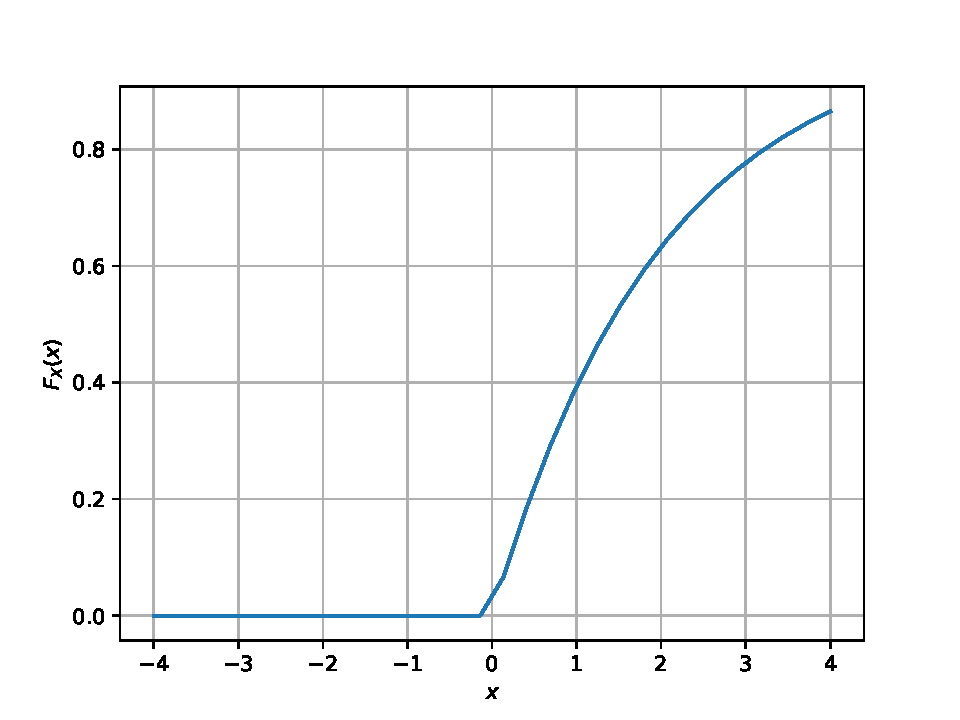
\includegraphics[width=\columnwidth]{/home/chinni/digitalc/figs/v_cdf.pdf}
\caption{CDF of $V$}
\label{fig:chisq_cdf}
\end{figure}
\begin{figure}[H]
\centering
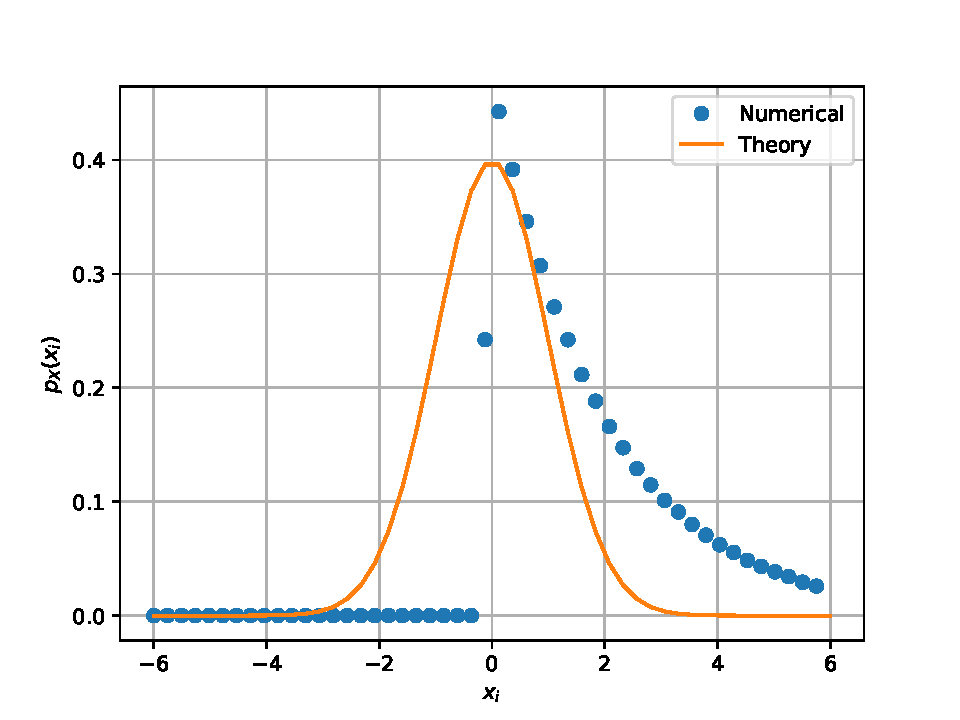
\includegraphics[width=\columnwidth]{/home/chinni/digitalc/figs/v_pdf.pdf}
\caption{PDF of $V$}
\label{fig:chisq_pdf}
\end{figure}
%
%
%
\item
If
%
\begin{equation}
\label{eq:chisq2_cdf_gen}
F_{V}(x) = 
\begin{cases}
1 - e^{-\alpha x} & x \geq 0 \\
0 & x < 0,
\end{cases}
\end{equation}
%
find $\alpha$.\\
\solution Let $Z=X^2$ where $X \sim \gauss{0}{1}$. Defining the CDF for $Z$,
\begin{flalign*}
	P_Z(z) &= \pr{Z < z}&\\
	&= \pr{X^2 < z}&\\
	&= \pr{-\sqrt{z} < X < \sqrt{z}}&\\
	&= \int_{-\sqrt{z}}^{\sqrt{z}} p_X(x)  \,dx 
\end{flalign*}
Using (5.2.3.1), the PDF of $Z$ is given by
\begin{align}
	\nonumber
	\frac{d}{dz}P_Z(z) &= p_Z(z)\\
	\label{eq:square_pdf_gen}
	= \frac{p_X(\sqrt{z})+p_X(-\sqrt{z})}{2\sqrt{z}} & \text{ (Using Lebniz's rule)} 
\end{align}
Substituting the standard gaussian density function $p_X(x) = \frac{1}{\sqrt{2\pi}}e^{-\frac{x^2}{2}}$ in \eqref{eq:square_pdf_gen},
\begin{equation}
\label{eq:chisq_pdf}
	p_Z(z) =
	\begin{cases}
	\frac{1}{\sqrt{2\pi z}}e^{-\frac{z}{2}} & z \ge 0\\
	0 & z < 0
	\end{cases} 
\end{equation}
The PDF of $X_1^2$ and $X_2^2$ are given by \eqref{eq:chisq_pdf}. Since $V$ is the sum of two independant random variables,
\begin{flalign*}
	p_V(v) &= p_{X_1^2}(x_1) \ast p_{X_2^2}(x_2)&\\
	&= \frac{1}{2\pi} \int_{0}^{v} \frac{e^{-\frac{x}{2}}}{\sqrt{x}}\frac{e^{-\frac{v-x}{2}}}{\sqrt{v-x}}  \,dx&\\
	&= \frac{e^{-\frac{v}{2}}}{2\pi} \int_{0}^{v} \frac{1}{\sqrt{x(v-x)}}  \,dx&\\
	&= \frac{e^{-\frac{v}{2}}}{2\pi} \sbrak{-\arcsin\left(\dfrac{v-2x}{v}\right)}_0^v&\\
	&= \frac{e^{-\frac{v}{2}}}{2\pi} \pi&\\
	&= \frac{e^{-\frac{v}{2}}}{2} \text{ for } v \ge 0
\end{flalign*}
$F_V(v)$ can be obtained from $p_V(v)$ using \eqref{eq:pdf_to_cdf}
\begin{flalign}
	\nonumber
	F_V(v) &= \frac{1}{2} \int_{0}^{v} \exp\left(-\frac{v}{2}\right)&\\
	\label{eq:chisq2_cdf}
	&= 1-\exp\left(-\frac{v}{2}\right) \text{ for } v \ge 0
\end{flalign}
Comparing \eqref{eq:chisq2_cdf} with \eqref{eq:chisq2_cdf_gen}, $\alpha = \frac{1}{2}$ 

%
\item
\label{ch3_raleigh_sim}
Plot the CDF and PDf of
%
\begin{equation}
A = \sqrt{V}
\end{equation}\\
\solution The CDF and PDF of $A$ are plotted in Fig.7.1.3.1 and Fig.7.1.3.2 respectively using the below codes
\begin{center}
\fbox{\parbox{10.5cm}{\href{https://github.com/Prathyushakorepu/FWC2/blob/main/Digital-communications/codes/G-to-other/A-cdf.py}{https://github.com/Prathyushakorepu/FWC2/blob/main\\/Digital-communications/codes/G-to-other/A-cdf.py}}}
\end{center}
\begin{center}
\fbox{\parbox{10.5cm}{\href{https://github.com/Prathyushakorepu/FWC2/blob/main/Digital-communications/codes/G-to-other/A-pdf.py}{https://github.com/Prathyushakorepu/FWC2/blob/main\\/Digital-communications/codes/G-to-other/A-pdf.py}}}
\end{center}
\begin{figure}[H]
\centering
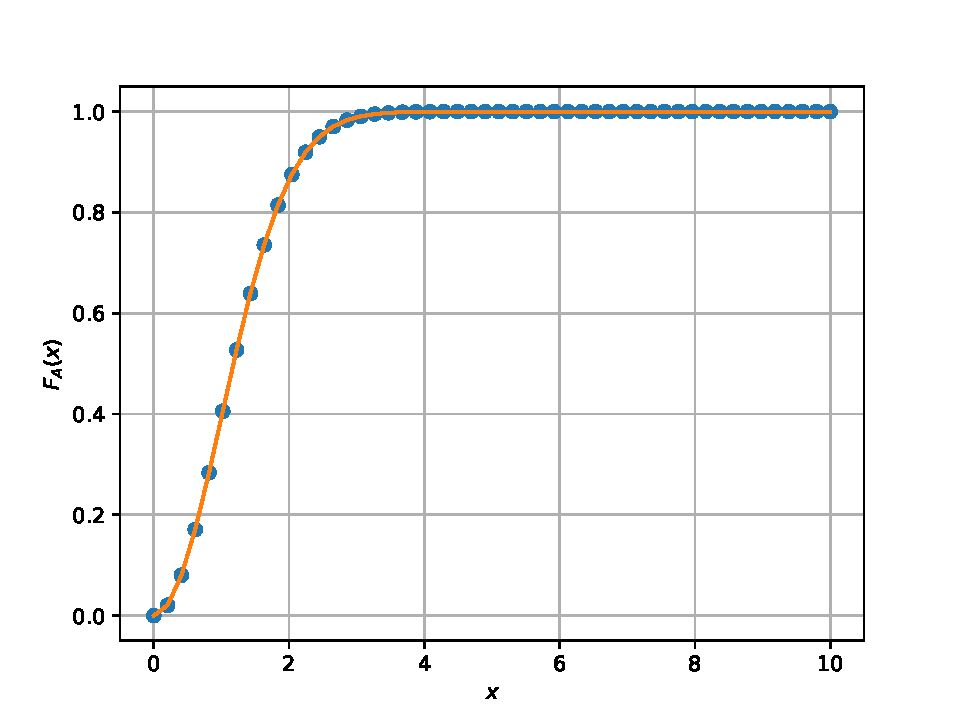
\includegraphics[width=\columnwidth]{/home/chinni/digitalc/figs/A_cdf.pdf}
\caption{CDF of $A$}
\label{fig:rayleigh_cdf}
\end{figure}
\begin{figure}[H]
\centering
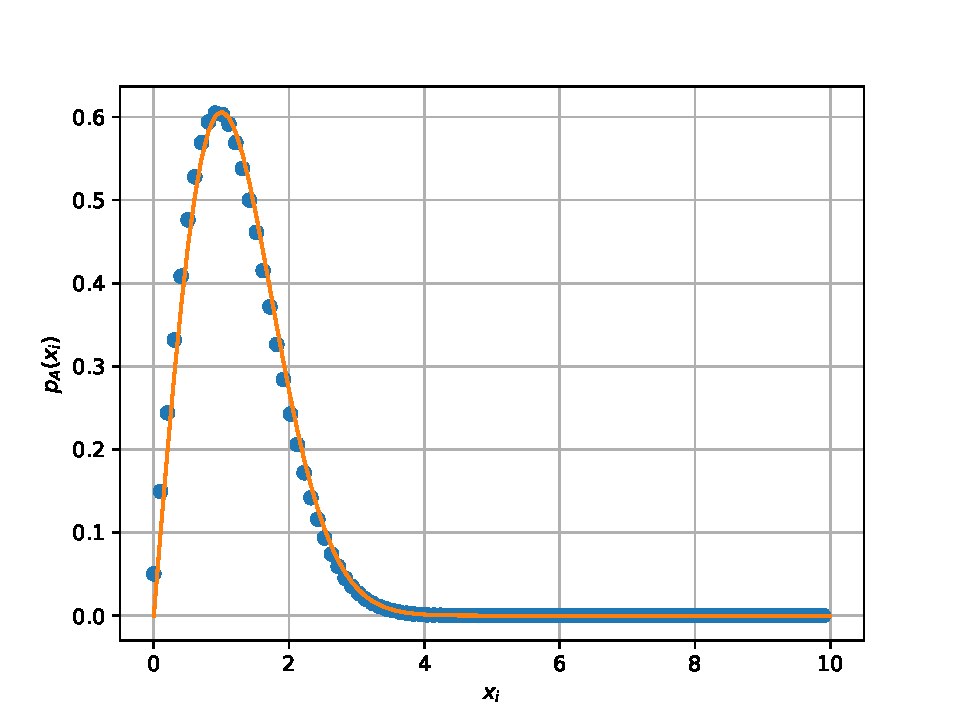
\includegraphics[width=\columnwidth]{/home/chinni/digitalc/figs/A_pdf.pdf}
\caption{PDF of $A$}
\label{fig:rayleigh_pdf}
\end{figure}
%
\end{enumerate}
\section{Conditional Probability}
\begin{enumerate}[label=\thesection.\arabic*
,ref=\thesection.\theenumi]
\item
\label{ch4_sim}
Plot 
\begin{equation}
P_e = \pr{\hat{X} = -1|X=1}
\end{equation}
%
for 
\begin{equation}
Y = AX+N,
\end{equation}
where $A$ is Raleigh with $E\sbrak{A^2} = \gamma, N \sim \gauss{0}{1}, X \in \brak{-1,1}$ for $0 \le \gamma \le 10$ dB.
\solution plotted in Fig.7.2.1.1  using the below code
\begin{center}
\fbox{\parbox{10.5cm}{\href{https://github.com/Prathyushakorepu/FWC2/blob/main/Digital-communications/codes/cond/cond-y.py}{https://github.com/Prathyushakorepu/FWC2/blob/main\\/Digital-communications/codes/cond/cond-y.py}}}
\end{center}
\begin{figure}[H]
\centering
\label{fig:bpsk_pe_snr_rayleigh}
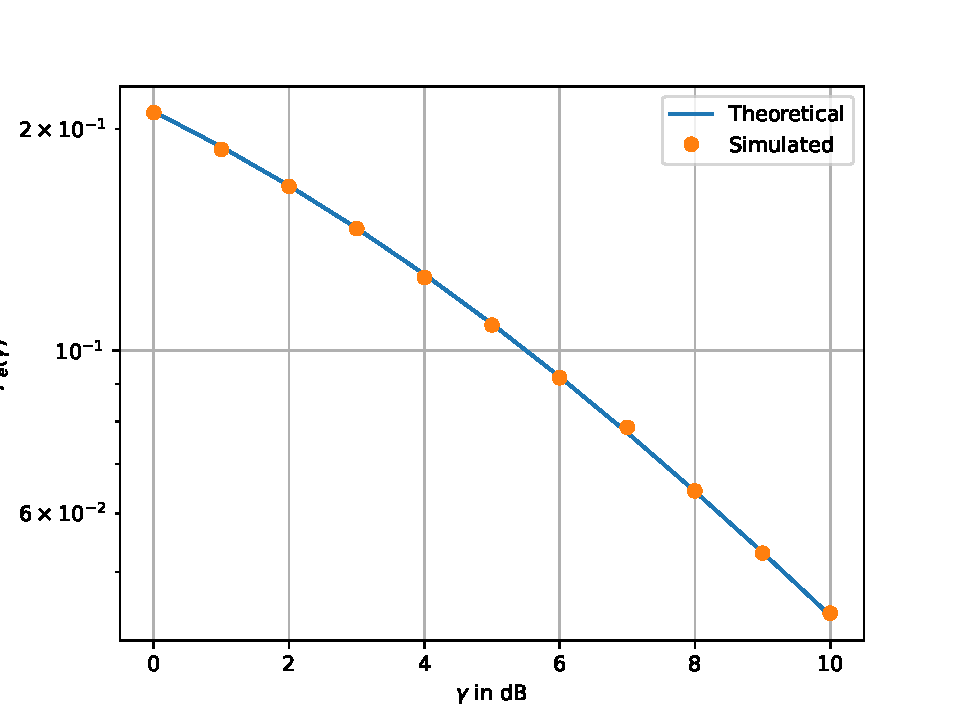
\includegraphics[width=\columnwidth]{/home/chinni/digitalc/figs/Pe_vs_gamma.pdf}
\caption{$P_e$ versus $\gamma$}
\end{figure}
%
\item
Assuming that $N$ is a constant, find an expression for $P_e$.  Call this $P_e(N)$\\
\solution Assuming the decision rule in \eqref{eq:bpsk_decision}, when $N$ is constant, $P_e$ is given by 
\begin{flalign}
	\nonumber
	P_e &= \pr{\hat{X} = -1|X=1}&\\ \nonumber
	&= \pr{Y<0|X=1}&\\ \nonumber
	&= \pr{AX+N<0|X=1}&\\ 
	\label{eq:prob_err_rayleigh_gen}
	&= \pr{A+N<0}&\\ \nonumber
	&= \pr{A<-N}&\\
	\label{eq:prob_err_bpsk_rayleigh_cdf}
	&=
	\begin{cases}
	F_A(-N) & N \ge 0\\
	0 & N < 0
	\end{cases}
\end{flalign}
For a Rayleigh random variable $X$ with $E\sbrak{X^2} = \gamma$, the PDF and CDF are given by
\begin{align}
	\label{eq:rayleigh_pdf}
	p_X(x) &= \frac{2x}{\gamma}\exp\left(-\frac{x^2}{\gamma}\right) \text{ for } x \ge 0\\
	\label{eq:rayleigh_cdf}
	F_X(X) &= 1-\exp\left(-\frac{x^2}{\gamma}\right) \text{ for } x \ge 0
\end{align}
Substituting \eqref{eq:rayleigh_cdf} in \eqref{eq:prob_err_bpsk_rayleigh_cdf},
\begin{equation}
	\label{eq:prob_err_bpsk_rayleigh_fN}
	P_e(N) =
	\begin{cases} 
	1-\exp\left(-\frac{N^2}{\gamma}\right) & N \ge 0\\
	0 & N < 0
	\end{cases}
\end{equation}
%
\item
%
\label{ch4_anal}
For a function $g$,
\begin{equation}
E\sbrak{g(X)} = \int_{-\infty}^{\infty}g(x)p_{X}(x)\, dx
\end{equation}
%
Find $P_e = E\sbrak{P_e(N)}$.\\
\solution Using $P_e(N)$ from \eqref{eq:prob_err_bpsk_rayleigh_fN},
\begin{flalign*}
	P_e &= \int_{-\infty}^{\infty} P_e(x)p_N(x) \,dx&\\
	&= \int_{0}^{\infty} \left(1-e^{-\frac{x^2}{\gamma}}\right)\frac{1}{\sqrt{2\pi}}e^{-\frac{x^2}{2}} \,dx
\end{flalign*}
	
\begin{multline*}
	P_e = \frac{1}{\sqrt{2\pi}}\int_{0}^{\infty} e^{-\frac{x^2}{2}}  \,dx \\ - \frac{1}{\sqrt{2\pi}}\int_{0}^{\infty} \exp\left(-x^2\left(\frac{1}{\gamma}+\frac{1}{2}\right)\right)  \,dx
\end{multline*}
\begin{flalign*}
	P_e &= \frac{1}{2} - \frac{1}{2}\sqrt{\frac{\gamma}{2+\gamma}}
\end{flalign*} 
%
\item
Plot $P_e$ in problems \ref{ch4_sim} and \ref{ch4_anal} on the same graph w.r.t $\gamma$.  Comment.\\
\solution $P_e$ plotted in same graph in Fig.7.2.1.1
		\end{enumerate}
		\iffalse
\section{Two Dimensions}
Let 
\begin{equation}
\mbf{y} = A\mbf{x} + \mbf{n},
\end{equation}
where 
\begin{align}
x &\in \brak{\mbf{s}_0,\mbf{s}_1}, 
\mbf{s}_0 = 
\begin{pmatrix}
1 
\\
0
\end{pmatrix},
\mbf{s}_1 = 
\begin{pmatrix}
0 
\\
1
\end{pmatrix}
\\
\mbf{n} &= 
\begin{pmatrix}
n_1
\\
n_2
\end{pmatrix},
n_1,n_2 \sim \gauss{0}{1}.
\end{align}
%
\begin{enumerate}[label=\thesection.\arabic*
,ref=\thesection.\theenumi]
%%
\item
\label{ch5_fsk}
Plot 
%
\begin{equation}
\mbf{y}|\mbf{s}_0 \text{ and } \mbf{y}|\mbf{s}_1
\end{equation}
%
on the same graph using a scatter plot.
%
\item
For the above problem, find a decision rule for detecting the symbols $\mbf{s}_0 $ and $\mbf{s}_1$.
%
\item
Plot 
\begin{equation} 
P_e = \pr{\hat{\mbf{x}} = \mbf{s}_1|\mbf{x} = \mbf{s}_0}
\end{equation}
with respect to the SNR from 0 to 10 dB.
%
\item
Obtain an expression for $P_e$. Verify this by comparing the theory and simulation plots on the same graph.
%
		\end{enumerate}
\end{document}
\fi


\chapter{Bivariate Random Variables: FSK}
\iffalse
\let\negmedspace\undefined
\let\negthickspace\undefined
\documentclass[journal,12pt,twocolumn]{IEEEtran}
%\documentclass[conference]{IEEEtran}
%\IEEEoverridecommandlockouts
% The preceding line is only needed to identify funding in the first footnote. If that is unneeded, please comment it out.
\usepackage{cite}
\usepackage{amssymb,amsfonts,amsthm,amsmath}
\usepackage{algorithmic}
\usepackage{graphicx}
\usepackage{textcomp}
\usepackage{xcolor}
\usepackage{txfonts}
\usepackage{listings}
\usepackage{enumitem}
\usepackage{mathtools}
\usepackage{gensymb}

%%
%\usepackage{setspace}
%%\doublespacing
%\singlespacing
%
%%\usepackage{graphicx}
%%\usepackage{amssymb}
%%\usepackage{relsize}
%\usepackage[cmex10]{amsmath}
%%\interdisplaylinepenalty=2500
%%\savesymbol{iint}
%%\usepackage{txfonts}
%%\restoresymbol{TXF}{iint}
%%\usepackage{wasysym}
%\usepackage{amsthm}
%\usepackage{mathrsfs}
%\usepackage{txfonts}
%%\usepackage{stfloats}
%%\usepackage{cite}
%%\usepackage{cases}
%%\usepackage{subfig}
%%\usepackage{xtab}
%%\usepackage{multirow}
%%\usepackage{algorithm}
%%\usepackage{algpseudocode}
%%\usepackage{tikz}
%%\usepackage{circuitikz}
%%\usepackage{verbatim}
\usepackage{hyperref}
%%\usepackage{stmaryrd}
%%\usepackage{tkz-euclide} % loads  TikZ and tkz-base
%%\usetkzobj{all}
    \usepackage{color}                                            %%
    \usepackage{array}                                            %%
    \usepackage{longtable}                                        %%
    \usepackage{calc}                                             %%
    \usepackage{multirow}                                         %%
    \usepackage{hhline}                                           %%
    \usepackage{ifthen}                                           %%
%  %optionally (for landscape tables embedded in another document): %%
%    \usepackage{lscape}     
%%\usepackage{multicol}
%\usepackage{chngcntr}
%\usepackage{enumerate}

%\usepackage{wasysym}
%\newcounter{MYtempeqncnt}
\DeclareMathOperator*{\Res}{Res}
%\renewcommand{\baselinestretch}{2}
\renewcommand\thesection{\arabic{section}}
\renewcommand\thesubsection{\thesection.\arabic{subsection}}
\renewcommand\thesubsubsection{\thesubsection.\arabic{subsubsection}}

\renewcommand\thesectiondis{\arabic{section}}
\renewcommand\thesubsectiondis{\thesectiondis.\arabic{subsection}}
\renewcommand\thesubsubsectiondis{\thesubsectiondis.\arabic{subsubsection}}

% correct bad hyphenation here
\hyphenation{op-tical net-works semi-conduc-tor}
\def\inputGnumericTable{}                                 %%

\lstset{
language=tex,
frame=single, 
breaklines=true
}

\begin{document}
%


\newtheorem{theorem}{Theorem}[section]
\newtheorem{problem}{Problem}
\newtheorem{proposition}{Proposition}[section]
\newtheorem{lemma}{Lemma}[section]
\newtheorem{corollary}[theorem]{Corollary}
\newtheorem{example}{Example}[section]
\newtheorem{definition}[problem]{Definition}
%\newtheorem{thm}{Theorem}[section] 
%\newtheorem{defn}[thm]{Definition}
%\newtheorem{algorithm}{Algorithm}[section]
%\newtheorem{cor}{Corollary}
\newcommand{\BEQA}{\begin{eqnarray}}
\newcommand{\EEQA}{\end{eqnarray}}
\newcommand{\define}{\stackrel{\triangle}{=}}
\bibliographystyle{IEEEtran}
%\bibliographystyle{ieeetr}
\providecommand{\mbf}{\mathbf}
\providecommand{\pr}[1]{\ensuremath{\Pr\left(#1\right)}}
\providecommand{\re}[1]{\ensuremath{\text{Re}\left(#1\right)}}
\providecommand{\im}[1]{\ensuremath{\text{Im}\left(#1\right)}}
\providecommand{\qfunc}[1]{\ensuremath{Q\left(#1\right)}}
\providecommand{\sbrak}[1]{\ensuremath{{}\left[#1\right]}}
\providecommand{\lsbrak}[1]{\ensuremath{{}\left[#1\right.}}
\providecommand{\rsbrak}[1]{\ensuremath{{}\left.#1\right]}}
\providecommand{\brak}[1]{\ensuremath{\left(#1\right)}}
\providecommand{\lbrak}[1]{\ensuremath{\left(#1\right.}}
\providecommand{\rbrak}[1]{\ensuremath{\left.#1\right)}}
\providecommand{\cbrak}[1]{\ensuremath{\left\{#1\right\}}}
\providecommand{\lcbrak}[1]{\ensuremath{\left\{#1\right.}}
\providecommand{\rcbrak}[1]{\ensuremath{\left.#1\right\}}}
\theoremstyle{remark}
\newtheorem{rem}{Remark}
\newcommand{\sgn}{\mathop{\mathrm{sgn}}}
\providecommand{\abs}[1]{\left\vert#1\right\vert}
\providecommand{\res}[1]{\Res\displaylimits_{#1}} 
\providecommand{\norm}[1]{\left\lVert#1\right\rVert}
%\providecommand{\norm}[1]{\lVert#1\rVert}
\providecommand{\mtx}[1]{\mathbf{#1}}
\providecommand{\mean}[1]{E\left[ #1 \right]}
\providecommand{\fourier}{\overset{\mathcal{F}}{ \rightleftharpoons}}
%\providecommand{\hilbert}{\overset{\mathcal{H}}{ \rightleftharpoons}}
\providecommand{\system}{\overset{\mathcal{H}}{ \longleftrightarrow}}
	%\newcommand{\solution}[2]{\textbf{Solution:}{#1}}
\newcommand{\solution}{\noindent \textbf{Solution: }}
\providecommand{\dec}[2]{\ensuremath{\overset{#1}{\underset{#2}{\gtrless}}}}
\newcommand{\myvec}[1]{\ensuremath{\begin{pmatrix}#1\end{pmatrix}}}
\newcommand{\mydet}[1]{\ensuremath{\begin{vmatrix}#1\end{vmatrix}}}
	\newcommand*{\permcomb}[4][0mu]{{{}^{#3}\mkern#1#2_{#4}}}
\newcommand*{\perm}[1][-3mu]{\permcomb[#1]{P}}
\newcommand*{\comb}[1][-1mu]{\permcomb[#1]{C}}
\providecommand{\gauss}[2]{\mathcal{N}\ensuremath{\left(#1,#2\right)}}
%%
%	%\newcommand{\solution}[2]{\textbf{Solution:}{#1}}
%\newcommand{\solution}{\noindent \textbf{Solution: }}
\newcommand{\cosec}{\,\text{cosec}\,}
\newcommand{\sinc}{\,\text{sinc}\,}
\newcommand{\rect}{\,\text{rect}\,}
%\numberwithin{equation}{section}
\numberwithin{equation}{subsection}
%\numberwithin{problem}{section}
%\numberwithin{definition}{section}
\makeatletter
\@addtoreset{figure}{problem}
\makeatother
\let\StandardTheFigure\thefigure
\let\vec\mathbf
\let\j\jmath
%\renewcommand{\thefigure}{\theproblem.\arabic{figure}}
\renewcommand{\thefigure}{\theproblem}
%\setlist[enumerate,1]{before=\renewcommand\theequation{\theenumi.\arabic{equation}}
%\counterwithin{equation}{enumi}
%\renewcommand{\theequation}{\arabic{subsection}.\arabic{equation}}
\def\putbox#1#2#3{\makebox[0in][l]{\makebox[#1][l]{}\raisebox{\baselineskip}[0in][0in]{\raisebox{#2}[0in][0in]{#3}}}}
     \def\rightbox#1{\makebox[0in][r]{#1}}
     \def\centbox#1{\makebox[0in]{#1}}
     \def\topbox#1{\raisebox{-\baselineskip}[0in][0in]{#1}}
     \def\midbox#1{\raisebox{-0.5\baselineskip}[0in][0in]{#1}}
\vspace{3cm}
\title{
%	\logo{
	Probability
%	}
}
%\title{
%	\logo{Matrix Analysis through Octave}{\begin{center}\includegraphics[scale=.24]{tlc}\end{center}}{}{HAMDSP}
%}
% paper title
% can use linebreaks \\ within to get better formatting as desired
%\title{Matrix Analysis through Octave}
%
%
% author names and IEEE memberships
% note positions of commas and nonbreaking spaces ( ~ ) LaTeX will not break
% a structure at a ~ so this keeps an author's name from being broken across
% two lines.
% use \thanks{} to gain access to the first footnote area
% a separate \thanks must be used for each paragraph as LaTeX2e's \thanks
% was not built to handle multiple paragraphs
%
\author{
	G. V. V. Sharma
	%<-this % stops a space
%\thanks{}}
}
% note the % following the last \IEEEmembership and also \thanks - 
% these prevent an unwanted space from occurring between the last author name
% and the end of the author line. i.e., if you had this:
% 
% \author{....lastname \thanks{...} \thanks{...} }
%                     ^------------^------------^----Do not want these spaces!
%
% a space would be appended to the last name and could cause every name on that
% line to be shifted left slightly. This is one of those "LaTeX things". For
% instance, "\textbf{A} \textbf{B}" will typeset as "A B" not "AB". To get
% "AB" then you have to do: "\textbf{A}\textbf{B}"
% \thanks is no different in this regard, so shield the last } of each \thanks
% that ends a line with a % and do not let a space in before the next \thanks.
% Spaces after \IEEEmembership other than the last one are OK (and needed) as
% you are supposed to have spaces between the names. For what it is worth,
% this is a minor point as most people would not even notice if the said evil
% space somehow managed to creep in.
% The paper headers
%\markboth{Journal of \LaTeX\ Class Files,~Vol.~6, No.~1, January~2007}%
%{Shell \MakeLowercase{\textit{et al.}}: Bare Demo of IEEEtran.cls for Journals}
% The only time the second header will appear is for the odd numbered pages
% after the title page when using the twoside option.
% 
% *** Note that you probably will NOT want to include the author's ***
% *** name in the headers of peer review papers.                   ***
% You can use \ifCLASSOPTIONpeerreview for conditional compilation here if
% you desire.
% If you want to put a publisher's ID mark on the page you can do it like
% this:
%\IEEEpubid{0000--0000/00\$00.00~\copyright~2007 IEEE}
% Remember, if you use this you must call \IEEEpubidadjcol in the second
% column for its text to clear the IEEEpubid mark.
% make the title area
\maketitle
\newpage
\tableofcontents
\bigskip
\renewcommand{\thefigure}{\theenumi}
\renewcommand{\thetable}{\theenumi}
%\renewcommand{\theequation}{\theenumi}
%\begin{abstract}
%%\boldmath
%In this letter, an algorithm for evaluating the exact analytical bit error rate  (BER)  for the piecewise linear (PL) combiner for  multiple relays is presented. Previous results were available only for upto three relays. The algorithm is unique in the sense that  the actual mathematical expressions, that are prohibitively large, need not be explicitly obtained. The diversity gain due to multiple relays is shown through plots of the analytical BER, well supported by simulations. 
%
%\end{abstract}
% IEEEtran.cls defaults to using nonbold math in the Abstract.
% This preserves the distinction between vectors and scalars. However,
% if the journal you are submitting to favors bold math in the abstract,
% then you can use LaTeX's standard command \boldmath at the very start
% of the abstract to achieve this. Many IEEE journals frown on math
% in the abstract anyway.
% Note that keywords are not normally used for peerreview papers.
%\begin{IEEEkeywords}
%Cooperative diversity, decode and forward, piecewise linear
%\end{IEEEkeywords}
% For peer review papers, you can put extra information on the cover
% page as needed:
% \ifCLASSOPTIONpeerreview
% \begin{center} \bfseries EDICS Category: 3-BBND \end{center}
% \fi
%
% For peerreview papers, this IEEEtran command inserts a page break and
% creates the second title. It will be ignored for other modes.
%\IEEEpeerreviewmaketitle
%\begin{abstract}
%\end{abstract}
%\iffalse
%% Copyright (C) 2020 Saurabh Joshi
%%% 
%\let\negmedspace\undefined
%\let\negthickspace\undefined
%
%\documentclass[journal,12pt,onecolumn]{IEEEtran}
%%\documentclass[journal,12pt,twocolumn]{IEEEtran}
%%
%\usepackage{setspace}
%\usepackage{gensymb}
%%\doublespacing
%\singlespacing
%
%%\usepackage{graphicx}
%%\usepackage{amssymb}
%%\usepackage{relsize}
%\usepackage[cmex10]{amsmath}
%%\usepackage{amsthm}
%%\interdisplaylinepenalty=2500
%%\savesymbol{iint}
%%\usepackage{txfonts}
%%\restoresymbol{TXF}{iint}
%%\usepackage{wasysym}
%\usepackage{amsthm}
%\usepackage{mathrsfs}
%\usepackage{txfonts}
%\usepackage{stfloats}
%\usepackage{cite}
%\usepackage{cases}
%\usepackage{subfig}
%%\usepackage{xtab}
%\usepackage{longtable}
%\usepackage{multirow}
%%\usepackage{algorithm}
%%\usepackage{algpseudocode}
%\usepackage{enumitem}
%\usepackage{mathtools}
%\usepackage{tikz}
%\usepackage{circuitikz}
%\usepackage{verbatim}
%\usepackage{hyperref}
%%\usepackage{stmaryrd}
%\usepackage{tkz-euclide} % loads  TikZ and tkz-base
%%\usetkzobj{all}
%\usepackage{listings}
%    \usepackage{color}                                            %%
%    \usepackage{array}                                            %%
%    \usepackage{longtable}                                        %%
%    \usepackage{calc}                                             %%
%    \usepackage{multirow}                                         %%
%    \usepackage{hhline}                                           %%
%    \usepackage{ifthen}                                           %%
%  %optionally (for landscape tables embedded in another document): %%
%    \usepackage{lscape}     
%\usepackage{multicol}
%\usepackage{chngcntr}
%\usepackage{iftex}
%%\usepackage[latin9]{inputenc}
%\usepackage{geometry}
%\usepackage{bm}
%%\geometry{verbose,tmargin=2cm,bmargin=3cm,lmargin=1.8cm,rmargin=1.5cm,headheight=2cm,headsep=2cm,footskip=3cm}
%\usepackage{array}
%\newcolumntype{L}[1]{>{\raggedright\let\newline\\\arraybackslash\hspace{0pt}}m{#1}}
%\newcolumntype{C}[1]{>{\centering\let\newline\\\arraybackslash\hspace{0pt}}m{#1}}
%\newcolumntype{R}[1]{>{\raggedleft\let\newline\\\arraybackslash\hspace{0pt}}m{#1}}
%
%%\usepackage{graphicx}
%%\usepackage{setspace}
%%\usepackage{parskip}
%
%\def \hsp {\hspace{3mm}}
%
%\makeatletter
%
%\providecommand{\tabularnewline}{\\}
%
%
%
%\makeatother
%\ifxetex
%\usepackage[T1]{fontenc}
%\usepackage{fontspec}
%%\setmainfont[ Path = fonts/]{Sanskrit_2003.ttf}
%\newfontfamily\nakulafont[Script=Devanagari,AutoFakeBold=2,Path = fonts/]{Nakula}
%%\newfontfamily\liberationfont{Liberation Sans Narrow}
%%\newfontfamily\liberationsansfont{Liberation Sans}
%\fi
%\usepackage{tikz}
%\usepackage{xcolor}
%%\usepackage{enumerate}
%
%%\usepackage{wasysym}
%%\newcounter{MYtempeqncnt}
%\DeclareMathOperator*{\Res}{Res}
%%\renewcommand{\baselinestretch}{2}
%\renewcommand\thesection{\arabic{section}}
%\renewcommand\thesubsection{\thesection.\arabic{subsection}}
%\renewcommand\thesubsubsection{\thesubsection.\arabic{subsubsection}}
%
%\renewcommand\thesectiondis{\arabic{section}}
%\renewcommand\thesubsectiondis{\thesectiondis.\arabic{subsection}}
%\renewcommand\thesubsubsectiondis{\thesubsectiondis.\arabic{subsubsection}}
%
%% correct bad hyphenation here
%\hyphenation{op-tical net-works semi-conduc-tor}
%\def\inputGnumericTable{}                                 %%
%
%\lstset{
%language=tex,
%frame=single, 
%breaklines=true
%}
%
%%\begin{document}
%%
%
%
%\newtheorem{theorem}{Theorem}[section]
%\newtheorem{problem}{Problem}
%\newtheorem{proposition}{Proposition}[section]
%\newtheorem{lemma}{Lemma}[section]
%\newtheorem{corollary}[theorem]{Corollary}
%\newtheorem{example}{Example}[section]
%\newtheorem{definition}[problem]{Definition}
%%\newtheorem{thm}{Theorem}[section] 
%%\newtheorem{defn}[thm]{Definition}
%%\newtheorem{algorithm}{Algorithm}[section]
%%\newtheorem{cor}{Corollary}
%\newcommand{\BEQA}{\begin{eqnarray}}
%\newcommand{\EEQA}{\end{eqnarray}}
%\newcommand{\define}{\stackrel{\triangle}{=}}
%
%\bibliographystyle{IEEEtran}
%%\bibliographystyle{ieeetr}
%
%
%\providecommand{\mbf}{\mathbf}
%\providecommand{\pr}[1]{\ensuremath{\Pr\left(#1\right)}}
%\providecommand{\qfunc}[1]{\ensuremath{Q\left(#1\right)}}
%\providecommand{\sbrak}[1]{\ensuremath{{}\left[#1\right]}}
%\providecommand{\lsbrak}[1]{\ensuremath{{}\left[#1\right.}}
%\providecommand{\rsbrak}[1]{\ensuremath{{}\left.#1\right]}}
%\providecommand{\brak}[1]{\ensuremath{\left(#1\right)}}
%\providecommand{\lbrak}[1]{\ensuremath{\left(#1\right.}}
%\providecommand{\rbrak}[1]{\ensuremath{\left.#1\right)}}
%\providecommand{\cbrak}[1]{\ensuremath{\left\{#1\right\}}}
%\providecommand{\lcbrak}[1]{\ensuremath{\left\{#1\right.}}
%\providecommand{\rcbrak}[1]{\ensuremath{\left.#1\right\}}}
%\theoremstyle{remark}
%\newtheorem{rem}{Remark}
%\newcommand{\sgn}{\mathop{\mathrm{sgn}}}
%\providecommand{\abs}[1]{\left\vert#1\right\vert}
%\providecommand{\res}[1]{\Res\displaylimits_{#1}} 
%\providecommand{\norm}[1]{\left\lVert#1\right\rVert}
%%\providecommand{\norm}[1]{\lVert#1\rVert}
%\providecommand{\mtx}[1]{\mathbf{#1}}
%\providecommand{\mean}[1]{E\left[ #1 \right]}
%%\numberwithin{equation}{section}
%\numberwithin{equation}{section}
%%\numberwithin{problem}{section}
%%\numberwithin{definition}{section}
%\makeatletter
%\@addtoreset{figure}{problem}
%\makeatother
%
%\let\StandardTheFigure\thefigure
%\let\vec\mathbf
%%\renewcommand{\thefigure}{\theproblem.\arabic{figure}}
%\renewcommand{\thefigure}{\theproblem}
%%\setlist[enumerate,1]{before=\renewcommand\theequation{\theenumi.\arabic{equation}}
%%\counterwithin{equation}{enumi}
%
%
%%\renewcommand{\theequation}{\arabic{subsection}.\arabic{equation}}
%
%\vspace{3cm}
%
%
%%\usepackage{babel}
%\begin{document}
%
%\begin{tabular}{L{6cm} C{5cm} R{5cm} }
%
%	\definecolor{circleorange}{rgb}{1,0.17,0.08}
%\definecolor{darkorange}{rgb}{1,0.27,0.1}
%\definecolor{orange2}{rgb}{1,0.5,0.15}
%\definecolor{orange3}{rgb}{1,0.65,0.25}
%\definecolor{yellow1}{rgb}{0.95,0.77,0.2}
%%\begin{tikzpicture}[scale=0.2,every node/.style={transform shape}]
%\begin{tikzpicture}[scale=0.1,every node/.style={transform shape}]
%\draw [fill=circleorange,circleorange] (5,10) circle (1.15); 
%\fill [darkorange] (5.06,8) -- (5.06,2) -- (7.3,1.2) -- (7.3,8.8) -- (5.06,8);
%\fill [darkorange] (4.94,8) -- (4.94,2) -- (2.7,1.2) -- (2.7,8.8) -- (4.94,8);
%\fill [orange2]    (7.4,8.4) -- (7.4,1.6) -- (8.2,1.2) -- (8.2,8.8) -- (7.4,8.4);
%\fill [orange2]    (2.6,8.4) -- (2.6,1.6) -- (1.8,1.2) -- (1.8,8.8) -- (2.6,8.4);
%\fill [orange3]    (8.3,8.4) -- (8.3,1.6) -- (9.0,1.2) -- (9.0,8.8) -- (8.3,8.4);
%\fill [orange3]    (1.7,8.4) -- (1.7,1.6) -- (1.0,1.2) -- (1.0,8.8) -- (1.7,8.4);
%\fill [yellow1]    (9.1,8.4) -- (9.1,1.6) -- (9.7,1.2) -- (9.7,8.8) -- (9.1,8.4);
%\fill [yellow1]    (0.9,8.4) -- (0.9,1.6) -- (0.3,1.2) -- (0.3,8.8) -- (0.9,8.4);
%\ifxetex
%\node [scale=2.1] at (5,-0.1)  {   {\bf {\nakulafont  भारतीय प्रौद्योगिकी संस्थान हैदराबाद }} };
%\node [scale=1.8] at (5,-1.2) {   {\bf { Indian Institute of Technology Hyderabad}} };
%%\node [scale=1.8] at (5,-1.2) {   {\bf {\liberationsansfont Indian Institute of Technology Hyderabad}} };
%\fi
%\end{tikzpicture}
%% \includegraphics[scale=0.05]{logo_iith} \newline
%
%& Assignments 
%	&
%	AI1110
%\end{tabular}
%
%
%\vspace{-6mm}
%\begin{center}
%%\includegraphics[scale=0.95]{Yellow-Line}
%\begin{tikzpicture}
%\definecolor{yellow1}{rgb}{0.95,0.77,0.2}
%\draw[line width=0.75mm, yellow1] (0,0) -- (\textwidth,0);
%\end{tikzpicture}
%\par\end{center}
		\numberwithin{equation}{enumi}
\section{Uniform Random Numbers}
Let $U$ be a uniform random variable between 0 and 1.
\begin{enumerate}[label=\thesection.\arabic*
,ref=\thesection.\theenumi]
\item Generate $10^6$ samples of $U$ using a C program and save into a file called uni.dat .
\\
\solution Download the following files and execute the  C program.
\begin{lstlisting}
codes/exrand.c
codes/coeffs.h
\end{lstlisting}
%
\item
Load the uni.dat file into python and plot the empirical CDF of $U$ using the samples in uni.dat. The CDF is defined as
\begin{align}
F_{U}(x) = \pr{U \le x}
\end{align}
\\
\solution  The following code plots Fig. \ref{fig:uni_cdf}
\begin{lstlisting}
codes/cdf_plot.py
\end{lstlisting}
\begin{figure}
\centering
\includegraphics[width=\columnwidth]{./figs/uni_cdf}
\caption{The CDF of $U$}
\label{fig:uni_cdf}
\end{figure}
%
\item
Find a  theoretical expression for $F_{U}(x)$.
\item
The mean of $U$ is defined as
%
\begin{equation}
E\sbrak{U} = \frac{1}{N}\sum_{i=1}^{N}U_i
\end{equation}
%
and its variance as
%
\begin{equation}
\text{var}\sbrak{U} = E\sbrak{U- E\sbrak{U}}^2 
\end{equation}
Write a C program to  find the mean and variance of $U$. 
\item Verify your result theoretically given that
%
\begin{equation}
E\sbrak{U^k} = \int_{-\infty}^{\infty}x^kdF_{U}(x)
\end{equation}
\end{enumerate}
\section{Central Limit Theorem}
%
\begin{enumerate}[label=\thesection.\arabic*
,ref=\thesection.\theenumi]
%
\item
Generate $10^6$ samples of the random variable
%
\begin{equation}
X = \sum_{i=1}^{12}U_i -6
\end{equation}
%
using a C program, where $U_i, i = 1,2,\dots, 12$ are  a set of independent uniform random variables between 0 and 1
and save in a file called gau.dat
%
\item
Load gau.dat in python and plot the empirical CDF of $X$ using the samples in gau.dat. What properties does a CDF have?
\\
\solution The CDF of $X$ is plotted in Fig. \ref{fig:gauss_cdf}
\begin{figure}
\centering
\includegraphics[width=\columnwidth]{./figs/gauss_cdf}
\caption{The CDF of $X$}
\label{fig:gauss_cdf}
\end{figure}
\item
Load gau.dat in python and plot the empirical PDF of $X$ using the samples in gau.dat. The PDF of $X$ is defined as
\begin{align}
p_{X}(x) = \frac{d}{dx}F_{X}(x)
\end{align}
What properties does the PDF have?
\\
\solution The PDF of $X$ is plotted in Fig. \ref{fig:gauss_pdf} using the code below
\begin{lstlisting}
codes/pdf_plot.py
\end{lstlisting}
\begin{figure}
\centering
\includegraphics[width=\columnwidth]{./figs/gauss_pdf}
\caption{The PDF of $X$}
\label{fig:gauss_pdf}
\end{figure}
\item Find the mean and variance of $X$ by writing a C program.
\item Given that 
\begin{align}
p_{X}(x) = \frac{1}{\sqrt{2\pi}}\exp\brak{-\frac{x^2}{2}}, -\infty < x < \infty,
\end{align}
repeat the above exercise theoretically.
%
\end{enumerate}
\section{From Uniform to Other}
\begin{enumerate}[label=\thesection.\arabic*
,ref=\thesection.\theenumi]
%
\item
Generate samples of 
%
\begin{equation}
V = -2\ln\brak{1-U}
\end{equation}
%
and plot its CDF.  
\item Find a theoretical expression for $F_V(x)$.
%
%\item
%Generate the Rayleigh distribution from Uniform. Verify your result through graphical plots.
\end{enumerate}
\section{Triangular Distribution}
\begin{enumerate}[label=\thesection.\arabic*
,ref=\thesection.\theenumi]
%
\item Generate 
	\begin{align}
		T = U_1+U_2
	\end{align}
\item Find the CDF of $T$.
\item Find the PDF of $T$.
\item Find the theoretical expressions for the PDF and CDF of $T$.
\item Verify your results through a plot. 
\end{enumerate}
\section{Maximum Likelihood}
\begin{enumerate}[label=\thesection.\arabic*
,ref=\thesection.\theenumi]
\item Generate equiprobable $X \in \cbrak{1,-1}$.
\item Generate 
\begin{equation}
Y = AX+N,
\end{equation}
		where $A = 5$ dB,  and $N \sim \gauss{0}{1}$.
	\item Plot $Y$ using a scatter plot.
	\item Guess how to estimate $X$ from $Y$.
\item
\label{ml-ch4_sim}
Find 
\begin{equation}
	P_{e|0} = \pr{\hat{X} = -1|X=1}
\end{equation}
and 
\begin{equation}
	P_{e|1} = \pr{\hat{X} = 1|X=-1}
\end{equation}
%
\item Find $P_e$ assuming that $X$ has equiprobable symbols.
%
\item
Verify by plotting  the theoretical $P_e$ with respect to $A$ from 0 to 10 dB.  
%
\item Now, consider a threshold $\delta$  while estimating $X$ from $Y$. Find the value of $\delta$ that maximizes the theoretical $P_e$.
\item Repeat the above exercise when 
	\begin{align}
		p_{X}(0) = p
	\end{align}
\item Repeat the above exercise using the MAP criterion.
		\end{enumerate}
\section{Gaussian to Other}
\begin{enumerate}[label=\thesection.\arabic*
,ref=\thesection.\theenumi]
\item
Let $X_1 \sim  \gauss{0}{1}$ and $X_2 \sim  \gauss{0}{1}$. Plot the CDF and PDF of
%
\begin{equation}
V = X_1^2 + X_2^2
\end{equation}
%
%
%
\item
If
%
\begin{equation}
F_{V}(x) = 
\begin{cases}
1 - e^{-\alpha x} & x \geq 0 \\
0 & x < 0,
\end{cases}
\end{equation}
%
find $\alpha$.
%
\item
\label{ch3_raleigh_sim}
Plot the CDF and PDf of
%
\begin{equation}
A = \sqrt{V}
\end{equation}
%
\end{enumerate}
\section{Conditional Probability}
\begin{enumerate}[label=\thesection.\arabic*
,ref=\thesection.\theenumi]
\item
\label{ch4_sim}
Plot 
\begin{equation}
P_e = \pr{\hat{X} = -1|X=1}
\end{equation}
%
for 
\begin{equation}
Y = AX+N,
\end{equation}
where $A$ is Raleigh with $E\sbrak{A^2} = \gamma, N \sim \gauss{0}{1}, X \in \brak{-1,1}$ for $0 \le \gamma \le 10$ dB.
%
\item
Assuming that $N$ is a constant, find an expression for $P_e$.  Call this $P_e(N)$
%
\item
%
\label{ch4_anal}
For a function $g$,
\begin{equation}
E\sbrak{g(X)} = \int_{-\infty}^{\infty}g(x)p_{X}(x)\, dx
\end{equation}
%
Find $P_e = E\sbrak{P_e(N)}$.
%
\item
Plot $P_e$ in problems \ref{ch4_sim} and \ref{ch4_anal} on the same graph w.r.t $\gamma$.  Comment.
		\end{enumerate}
		\fi
\section{Two Dimensions}
Let 
\begin{equation}
\mbf{y} = A\mbf{x} + \mbf{n},
\end{equation}
where 
\begin{align}
x &\in \brak{\mbf{s}_0,\mbf{s}_1}, 
\mbf{s}_0 = 
\begin{pmatrix}
1 
\\
0
\end{pmatrix},
\mbf{s}_1 = 
\begin{pmatrix}
0 
\\
1
\end{pmatrix}
\\
\mbf{n} &= 
\begin{pmatrix}
n_1
\\
n_2
\end{pmatrix},
n_1,n_2 \sim \gauss{0}{1}.
\end{align}
%
\begin{enumerate}[label=\thesection.\arabic*
,ref=\thesection.\theenumi]
%%
\item
\label{ch5_fsk}
Plot 
%
\begin{equation}
\mbf{y}|\mbf{s}_0 \text{ and } \mbf{y}|\mbf{s}_1
\end{equation}
%
on the same graph using a scatter plot.\\
\solution The scatter plot in Fig.8.1.1.1 is generated using the below code,
\begin{center}
\fbox{\parbox{10.5cm}{\href{https://github.com/Prathyushakorepu/FWC2/blob/main/Digital-communications/codes/Two-dimentions/scatter-plt.py}{https://github.com/Prathyushakorepu/FWC2/blob/main\\/Digital-communications/codes/Two-dimentions/scatter-plt.py}}}
\end{center}
%
\begin{figure}[H]
\centering
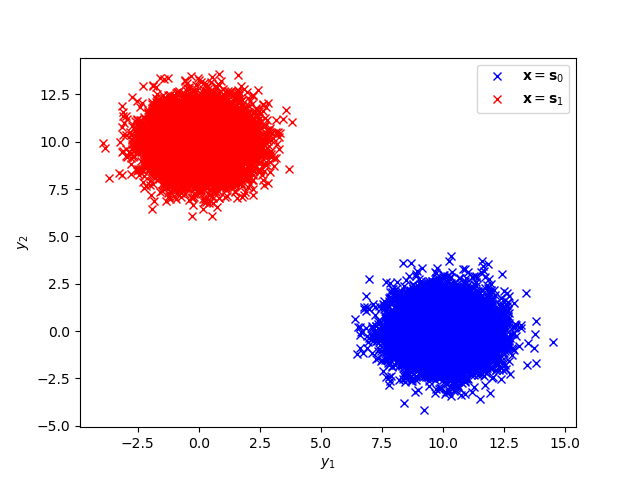
\includegraphics[width=\columnwidth]{/home/chinni/digitalc/figs/scatter_plot.png}
\caption{Scatter plot of $y$ }
\label{fig:biv_scatter}
\end{figure}
%
\item
For the above problem, find a decision rule for detecting the symbols $\mbf{s}_0 $ and $\mbf{s}_1$.\\
\solution Let $\mbf{y} = \myvec{y_1&y_2}^T$. Then the decision rule is
\begin{equation}
	y_1 \dec{0}{1} y_2
	\label{eq:biv_fsk_decision}
\end{equation}
$\vec{y}|\vec{s}_i$ is a random vector with each of its components normally distributed. The PDF of $\vec{y}|\vec{s}_i$ is given by,
\begin{equation}
	p_{\vec{y}|\vec{s}_i}\brak{\vec{y}} = \frac{1}{2\pi\sqrt{\mydet{\vec{\Sigma}}}} \exp\brak{-\frac{1}{2}\brak{\vec{y}-\vec{s}_i}^\top \vec{\Sigma}^{-1} \brak{\vec{y}-\vec{s}_i}}
\end{equation}
Where $\vec{\Sigma}$ is the covariance matrix. Substituting $\vec{\Sigma} = \sigma \vec{I}$,
\begin{align}
	p_{\vec{y}|\vec{s}_i}\brak{\vec{y}} &= \frac{1}{2 \pi \sigma} \exp\brak{-\frac{1}{2 \sigma}\brak{\vec{y}-\vec{s}_i}^\top \vec{I} \brak{\vec{y}-\vec{s}_i}}\\
	&= \frac{1}{2 \pi \sigma} \exp\brak{-\frac{1}{2 \sigma}\brak{\vec{y}-\vec{s}_i}^\top \brak{\vec{y}-\vec{s}_i}}
\end{align}
Assuming equiprobable symbols, use MAP rule in \eqref{eq:map_rule} to find optimum decision. Since there are only two possible symbols %
$\vec{s}_0$ and $\vec{s}_1$, the optimal decision criterion is found by equating $p_{\vec{y}|\vec{s}_0}$ and $p_{\vec{y}|\vec{s}_1}$.
\begin{align*}
	p_{\vec{y}|\vec{s}_0} &= p_{\vec{y}|\vec{s}_1}
\end{align*}
	
\begin{multline*}
	\implies \exp\brak{-\frac{1}{2 \sigma}\brak{\vec{y}-\vec{s}_0}^\top \brak{\vec{y}-\vec{s}_0}} = \\
	\exp\brak{-\frac{1}{2 \sigma}\brak{\vec{y}-\vec{s}_1}^\top \brak{\vec{y}-\vec{s}_1}}
\end{multline*}
	
\begin{align*}
	\implies \brak{\vec{y}-\vec{s}_0}^\top \brak{\vec{y}-\vec{s}_0} &= \brak{\vec{y}-\vec{s}_1}^\top \brak{\vec{y}-\vec{s}_1}\\
	\implies \vec{y}^\top\vec{y} - 2\vec{s}_0^\top \vec{y} + \vec{s}_0^T\vec{s}_0 &= \vec{y}^\top\vec{y} - 2\vec{s}_1^\top \vec{y} + \vec{s}_1^T\vec{s}_1\\
	\implies 2\brak{\vec{s}_1-\vec{s}_0}^\top \vec{y} &= \norm{\vec{s}_1}^2 - \norm{\vec{s}_0}^2\\
	\implies \brak{\vec{s}_1-\vec{s}_0}^\top \vec{y} &= 0\\
	\implies \myvec{-1\\1}^\top \vec{y} &= 0
\end{align*}

%
\item
Plot 
\begin{equation} 
P_e = \pr{\hat{\mbf{x}} = \mbf{s}_1|\mbf{x} = \mbf{s}_0}
\end{equation}
with respect to the SNR from 0 to 10 dB.\\
\solution The blue dots in Fig.8.1.3.1 are the $P_e$ versus SNR plot. It is generated using the below code,
\begin{center}
\fbox{\parbox{10.5cm}{\href{https://github.com/Prathyushakorepu/FWC2/blob/main/Digital-communications/codes/Two-dimentions/ber-snr.py}{https://github.com/Prathyushakorepu/FWC2/blob/main\\/Digital-communications/codes/Two-dimentions/ber-snr.py}}}
\end{center}
\begin{figure}[H]
\centering
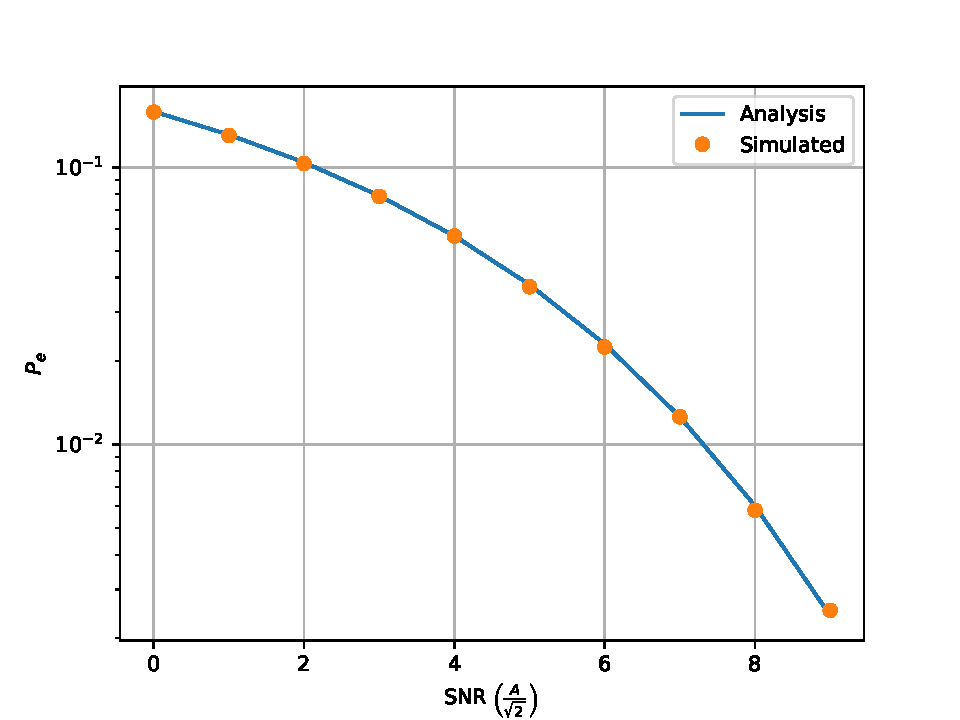
\includegraphics[width=\columnwidth]{/home/chinni/digitalc/figs/ber_snr_plot.pdf}
\caption{$P_e$ versus SNR plot for FSK}
\label{fig:biv_pe_snr}
\end{figure}

%
\item
Obtain an expression for $P_e$. Verify this by comparing the theory and simulation plots on the same graph.\\
\solution Using the decision rule from \eqref{eq:biv_fsk_decision},
\begin{align}
	\nonumber
	P_e &= \pr{\hat{\mbf{x}} = \mbf{s}_1|\mbf{x} = \mbf{s}_0}\\\nonumber
	&= \pr{y_1 < y_2|\mbf{x} = \mbf{s}_0}\\\nonumber
	&= \pr{A+n_1 < n_2}\\
	\label{eq:prob_error_fsk_inter}
	&= \pr{n_1-n_2 < -A}
\end{align}
%\textbf{Theorem:} The sum of $N$ independant random variables $X_1,X_2,...,X_N$ with $X_i \sim \gauss{\mu_i}{\sigma_i}$ is itself normally distributed %
%with $\mu =\sum_{i=1}^n \mu_i$ and $\sigma^2 = \sum_{i=1}^n \sigma_i^2$.\\
Let $Z = n_1-n_2$ where $n_1, n_2 \sim \gauss{0}{\sigma^2}$. The PDF of X is given by,
\begin{align}
	\nonumber
	p_Z(z) &= p_{n_1}(n_1) \ast p_{-n_2}(n_2)\\\nonumber
	&= \frac{1}{2\pi\sigma^2}\int_{-\infty}^{\infty} e^{-\frac{t^2}{2\sigma^2}}e^{-\frac{(t-z)^2}{2\sigma^2}}  \,dt\\\nonumber
	&= \frac{1}{2\pi\sigma^2}\int_{-\infty}^{\infty} e^{-\frac{(z-t)^2+t^2}{2\sigma^2}}  \,dt\\\nonumber
	&= \frac{1}{2\pi\sigma^2}\int_{-\infty}^{\infty} e^{-\frac{(2t-z)^2+z^2}{2(\sqrt{2}\sigma)^2}}  \,dt\\\nonumber
	&= \frac{1}{2\pi\sigma^2}e^{-\frac{z^2}{2(\sqrt{2}\sigma)^2}}\int_{-\infty}^{\infty} e^{-\frac{(2t-z)^2}{2(\sqrt{2}\sigma)^2}}  \,dt\\\nonumber
	&= \frac{e^{-\frac{z^2}{2(\sqrt{2}\sigma)^2}}}{\sqrt{2\pi}\sqrt{2}\sigma} \frac{1}{\sqrt{2\pi}\sqrt{2}\sigma}\int_{-\infty}^{\infty} e^{-\frac{k^2}{2(\sqrt{2}\sigma)^2}}  \,dk\\
	\label{eq:std_gauss_diff_pdf_fsk}
	&= \frac{e^{-\frac{z^2}{2(\sqrt{2}\sigma)^2}}}{\sqrt{2\pi}\sqrt{2}\sigma}
\end{align}
From \eqref{eq:std_gauss_diff_pdf_fsk}, $Z \sim \gauss{0}{2\sigma^2}$. Substituting $\sigma=1$, $Z \sim \gauss{0}{2}$. %
\eqref{eq:prob_error_fsk_inter} can be further simplified as,
\begin{align*}
	P_e &= \pr{Z < -A}&\\
	&= \pr{Z > A}&\\
	&= \qfunc{\frac{A}{\sqrt{2}}}&\\
	&= \frac{1}{\sqrt{2\pi}}\int_{\frac{A}{\sqrt{2}}}^{\infty} \exp\left(-\frac{x^2}{2}\right)  \,dx 
\end{align*}
Fig.8.1.3.1 compares the theoretical and simulation plots.

%
		\end{enumerate}
		\iffalse
\end{document}
\fi


%\chapter{Exercises}
%\iffalse
\documentclass[journal,12pt,twocolumn]{IEEEtran}
%
\usepackage{setspace}
\usepackage{gensymb}
\usepackage{xcolor}
\usepackage{caption}
%\usepackage{subcaption}
%\doublespacing
\singlespacing
\usepackage{multicol}

\usepackage{iithtlc}
%\usepackage{graphicx}
%\usepackage{amssymb}
%\usepackage{relsize}
\usepackage[cmex10]{amsmath}
\usepackage{mathtools}
%\usepackage{amsthm}
%\interdisplaylinepenalty=2500
%\savesymbol{iint}
%\usepackage{txfonts}
%\restoresymbol{TXF}{iint}
%\usepackage{wasysym}
\usepackage{amsthm}
\usepackage{mathrsfs}
\usepackage{txfonts}
\usepackage{stfloats}
\usepackage{cite}
\usepackage{cases}
\usepackage{subfig}
%\usepackage{xtab}
\usepackage{longtable}
\usepackage{multirow}
%\usepackage{algorithm}
%\usepackage{algpseudocode}
\usepackage{enumitem}
\usepackage{mathtools}
%\usepackage{stmaryrd}

\usepackage{listings}
    \usepackage[latin1]{inputenc}                                 %%
    \usepackage{color}                                            %%
    \usepackage{array}                                            %%
    \usepackage{longtable}                                        %%
    \usepackage{calc}                                             %%
    \usepackage{multirow}                                         %%
    \usepackage{hhline}                                           %%
    \usepackage{ifthen}                                           %%
  %optionally (for landscape tables embedded in another document): %%
    \usepackage{lscape}     

%\usepackage{wasysym}
%\newcounter{MYtempeqncnt}
\DeclareMathOperator*{\Res}{Res}
%\renewcommand{\baselinestretch}{2}
\renewcommand\thesection{\arabic{section}}
\renewcommand\thesubsection{\thesection.\arabic{subsection}}
\renewcommand\thesubsubsection{\thesubsection.\arabic{subsubsection}}

\renewcommand\thesectiondis{\arabic{section}}
\renewcommand\thesubsectiondis{\thesectiondis.\arabic{subsection}}
\renewcommand\thesubsubsectiondis{\thesubsectiondis.\arabic{subsubsection}}

% correct bad hyphenation here
\hyphenation{op-tical net-works semi-conduc-tor}

\def\inputGnumericTable{}  

\lstset{
language=python,
frame=single, 
breaklines=true
}

\begin{document}
%

\theoremstyle{definition}

\newtheorem{theorem}{Theorem}[section]
\newtheorem{problem}{Problem}
\newtheorem{proposition}{Proposition}[section]
\newtheorem{lemma}{Lemma}[section]
\newtheorem{corollary}[theorem]{Corollary}
\newtheorem{example}{Example}[section]
\newtheorem{definition}{Definition}[section]
%\newtheorem{algorithm}{Algorithm}[section]
%\newtheorem{cor}{Corollary}
\newcommand{\BEQA}{\begin{eqnarray}}
\newcommand{\EEQA}{\end{eqnarray}}
\newcommand{\triangleq}{\stackrel{\triangle}{=}}
\bibliographystyle{IEEEtran}
%\bibliographystyle{ieeetr}
\providecommand{\pr}[1]{\ensuremath{\Pr\left(#1\right)}}
\providecommand{\qfunc}[1]{\ensuremath{Q\left(#1\right)}}
\providecommand{\sbrak}[1]{\ensuremath{{}\left[#1\right]}}
\providecommand{\lsbrak}[1]{\ensuremath{{}\left[#1\right.}}
\providecommand{\rsbrak}[1]{\ensuremath{{}\left.#1\right]}}
\providecommand{\brak}[1]{\ensuremath{\left(#1\right)}}
\providecommand{\lbrak}[1]{\ensuremath{\left(#1\right.}}
\providecommand{\rbrak}[1]{\ensuremath{\left.#1\right)}}
\providecommand{\cbrak}[1]{\ensuremath{\left\{#1\right\}}}
\providecommand{\lcbrak}[1]{\ensuremath{\left\{#1\right.}}
\providecommand{\rcbrak}[1]{\ensuremath{\left.#1\right\}}}
\theoremstyle{remark}
\newtheorem{rem}{Remark}
\newcommand{\sgn}{\mathop{\mathrm{sgn}}}
\providecommand{\abs}[1]{\left\vert#1\right\vert}
\providecommand{\res}[1]{\Res\displaylimits_{#1}} 
\providecommand{\norm}[1]{\lVert#1\rVert}
\providecommand{\mtx}[1]{\mathbf{#1}}
\providecommand{\mean}[1]{E\left[ #1 \right]}
\providecommand{\fourier}{\overset{\mathcal{F}}{ \rightleftharpoons}}
%\providecommand{\hilbert}{\overset{\mathcal{H}}{ \rightleftharpoons}}
\providecommand{\system}{\overset{\mathcal{H}}{ \longleftrightarrow}}
\providecommand{\gauss}[2]{\mathcal{N}\ensuremath{\left(#1,#2\right)}}
	%\newcommand{\solution}[2]{\textbf{Solution:}{#1}}
\newcommand{\solution}{\noindent \textbf{Solution: }}
\providecommand{\dec}[2]{\ensuremath{\overset{#1}{\underset{#2}{\gtrless}}}}
%\numberwithin{equation}{section}
%\numberwithin{problem}{section}
\def\putbox#1#2#3{\makebox[0in][l]{\makebox[#1][l]{}\raisebox{\baselineskip}[0in][0in]{\raisebox{#2}[0in][0in]{#3}}}}
     \def\rightbox#1{\makebox[0in][r]{#1}}
     \def\centbox#1{\makebox[0in]{#1}}
     \def\topbox#1{\raisebox{-\baselineskip}[0in][0in]{#1}}
     \def\midbox#1{\raisebox{-0.5\baselineskip}[0in][0in]{#1}}
% paper title
% can use linebreaks \\ within to get better formatting as desired
\title{
%\logo{
Digital Modulation Techniques
%}
}
%
%
% author names and IEEE memberships
% note positions of commas and nonbreaking spaces ( ~ ) LaTeX will not break
% a structure at a ~ so this keeps an author's name from being broken across
% two lines.
% use \thanks{} to gain access to the first footnote area
% a separate \thanks must be used for each paragraph as LaTeX2e's \thanks
% was not built to handle multiple paragraphs
%
%\author{Y Aditya, A Rathnakar and G V V Sharma$^{*}$% <-this % stops a space
\author{P.~N.~V.~S.~S.~K.~ HAVISH, S.~S.~Ashish and G V V Sharma %<-this  stops a space
\thanks{The authors are with the Department
of Electrical Engineering, IIT, Hyderabad
502285 India e-mail: \{ee16btech11023,ee16btech11043,jbala,gadepall\}@iith.ac.in. All material in the manuscript is released under GNU GPL.  Free to use for all.
}}
% make the title area
\maketitle
\tableofcontents
\bigskip
\begin{abstract}
%\boldmath
The manual frames the problems of receiver design and performance analysis in digital communication as applications of probability theory.
\end{abstract}
% IEEEtran.cls defaults to using nonbold math in the Abstract.
% This preserves the distinction between vectors and scalars. However,
% if the journal you are submitting to favors bold math in the abstract,
% then you can use LaTeX's standard command \boldmath at the very start
% of the abstract to achieve this. Many IEEE journals frown on math
% in the abstract anyway.
% Note that keywords are not normally used for peerreview papers.
%\begin{IEEEkeywords}
%Cooperative diversity, decode and forward, piecewise linear
%\end{IEEEkeywords}
% For peer review papers, you can put extra information on the cover
% page as needed:
% \ifCLASSOPTIONpeerreview
% \begin{center} \bfseries EDICS Category: 3-BBND \end{center}
% \fi
%
% For peerreview papers, this IEEEtran command inserts a page break and
% creates the second title. It will be ignored for other modes.
\IEEEpeerreviewmaketitle
\fi
\section{BPSK}
\begin{enumerate}
\item
The {\em signal constellation diagram} for BPSK is given by Fig. \ref{fig:bpsk_const}.  The symbols $s_0$ and $s_1$ are equiprobable.  $\sqrt{E_b}$ is the energy transmitted per bit. Assuming a zero mean additive white gaussian noise (AWGN) with variance $\frac{N_0}{2}$,
obtain the symbols that are received.
%
\begin{figure}[!h]
\centering
%%%\includegraphics[scale=0.5]{../../digitalc/figs/bfsk_const.eps} 
%\includegraphics[width=\columnwidth]{/home/chinni/digitalc/figs/bpsk_const.eps}
\caption{}
\label{fig:bpsk_const}
\end{figure}
\solution The possible received symbols are
\begin{align}
y|s_0 &= \sqrt{E_b} + n
\\
y|s_1 &= -\sqrt{E_b} + n
\end{align}
%
where the AWGN $n \sim \gauss{0}{\frac{N_0}{2}}$.
%
\item
\label{prob:bpsk_decision}
From Fig. \ref{fig:bpsk_const} obtain a decision rule for BPSK
\solution The decision rule is
\begin{equation}
y \dec{s_0}{s_1} 0
\end{equation}
\item
Repeat the previous exercise using the MAP criterion.
\item
Using the decision rule in Problem \ref{prob:bpsk_decision}, obtain an expression for the probability of error for BPSK.
\solution
Since the symbols are equiprobable, it is sufficient if the error is calculated assuming that a 0 was sent.  This results in
\begin{align}
P_e &= \pr{y < 0|s_0} = \pr{\sqrt{E_b} + n < 0}
\\
&= \pr{ -n > \sqrt{E_b} } = \pr{ n > \sqrt{E_b} }
\label{eq:bpsk_proof_n0}
\end{align}
since $n$ has a symmetric pdf.
Let $w \sim \gauss{0}{1}$.  Then $n = \sqrt{\frac{N_0}{2}}w$. Substituting this in \eqref{eq:bpsk_proof_n0},
\begin{align}
P_e &=  \pr{ \sqrt{\frac{N_0}{2}}w > \sqrt{E_b} } = \pr{ w > \sqrt{\frac{2E_b}{N_0}} }
\\
&= \qfunc{\sqrt{\frac{2E_b}{N_0}}}
\end{align}
%
where $\qfunc{x} \triangleq \pr{w > x}, x \ge 0$.
\item
The PDF of $w \sim \gauss{0}{1}$ is given by
%
\begin{equation}
p_{w}(x) = \frac{1}{\sqrt{2\pi}}\exp\brak{-\frac{x^2}{2}}, -\infty < x < \infty
\end{equation}
and the complementary error function is defined as
\begin{equation}
\operatorname {erfc} (x)={\frac {2}{\sqrt {\pi }}}\int _{x}^{\infty }e^{-t^{2}}\,dt.
\end{equation}
%
Show that 
\begin{equation}
Q(x) = \frac{1}{2}\operatorname {erfc}\left({\frac  {x}{{\sqrt  {2}}}}\right)
\end{equation}
\item
Verify the bit error rate (BER) plots for BPSK through simulation and analysis for 0 to 10 dB.
\solution
The following code
%\lstinputlisting{./codes/bpsk_ber.py}
%\iffalse
\begin{lstlisting}
codes/bpsk_ber.py
\end{lstlisting}
%	\fi
yields Fig. \ref{fig:bpsk_ber}
\begin{figure}[!h]
\centering
%%%\includegraphics[width=\columnwidth]{./manual/figs/bpsk_ber.eps}
\caption{}
\label{fig:bpsk_ber}
\end{figure}
\item
Show that
\begin{equation}
Q(x) = \frac{1}{\pi}\int^{\frac{\pi}{2}}_{0}e^{-\frac{x^2}{2\sin^2 \theta}}\,d\theta
\end{equation}
\end{enumerate}
\section{Coherent BFSK}
\begin{enumerate}
\item
The signal constellation for binary frequency shift keying (BFSK) is given in Fig. \ref{fig:bfsk_const}.
Obtain the equations for the received symbols.
\begin{figure}[!h]
\centering
%%%\includegraphics[width=\columnwidth]{./manual/figs/bfsk_const.eps}
\caption{}
\label{fig:bfsk_const}
\end{figure}
\solution
The received symbols are given by
\begin{align}
\mathbf{y}|s_0 = 
\myvec{
\sqrt{E_b} \\
0
}
+
\myvec{
 n_{1}\\
n_{2}
},
\end{align}
and 
\begin{align}
\mathbf{y}|s_1 = 
\myvec{
0\\
\sqrt{E_b} 
}
+
\myvec{
n_{1}\\
 n_{2}
},
\end{align}
where $n_1,n_2 \sim \gauss{0}{\frac{N_0}{2}}$. and
$
\mathbf{y} = 
\myvec{
y_{1}\\
 y_{2}
}
$.
\item
Obtain a decision rule for BFSK from Fig. \ref{fig:bfsk_const}.
\solution The decision rule is
\begin{equation}
y_1 \dec{s_0}{s_1} y_2
\end{equation}
\item
Repeat the previous exercise using the MAP criterion.
\item
Derive and plot the probability of error.  Verify through simulation.
\end{enumerate}
%
\section{QPSK}
\begin{enumerate}
\item
Let
\begin{equation}
\mathbf{r} = \mathbf{s}+ \mathbf{n}
\end{equation}
where $\mathbf{s} \in \cbrak{s_0,s_1,s_2, s_3}$ and
\begin{align}
\mathbf{s}_0 &= 
\myvec{
\sqrt{E_b}\\
0
},
\mathbf{s}_1 = 
\myvec{
0\\
\sqrt{E_b}
},
\\
\mathbf{s}_2 &= 
\myvec{
-\sqrt{E_b}\\
0
},
\mathbf{s}_3 = 
\myvec{
0\\
-\sqrt{E_b}
},
\\
E\sbrak{\mathbf{n}} &= \mathbf{0}, E\sbrak{\mathbf{n}\mathbf{n}^T} = \sigma^2 \mathbf{I}
\end{align}
%
\begin{enumerate}
\item Show that the MAP decision for detecting $\mathbf{s}_0$ results in
\begin{equation}
\abs{r}_2 < r_1
\end{equation}
\item Express $\pr{\hat{\mathbf{s}} = \mathbf{s}_0|\mathbf{s} = \mathbf{s}_0}$ in terms of $r_1, r_2$.
Let $X=n_2-n_1, Y = -n_2-n_1$, where $\mathbf{n}=\brak{n_1,n_2}$.
Their correlation coefficient is defined as
%
\begin{align}
\rho = \frac{E\sbrak{\brak{X-\mu_x}\brak{Y-\mu_y}}}{\sigma_x\sigma_y}
\end{align}
%
$X$ and $Y$ are said to be uncorrelated if $\rho = 0$
\item Show that if $X$ and $Y$ are uncorrelated 
Verify this numerically.
\item Show that $X$ and $Y$ are independent, i.e. $p_{XY}(x,y) = p_{X}(x)p_{Y}(y)$.
\item Show that $X,Y \sim \mathcal{N}\brak{0,2\sigma^2}$.
\item Show that $\pr{\hat{\mathbf{s}} = \mathbf{s}_0|\mathbf{s} = \mathbf{s}_0} =\pr{ X < A,  Y < A}$.
\item Find $\pr{ X < A,  Y < A}$.
\item Verify the above through simulation.
\end{enumerate}
\end{enumerate}
\section{$M$-PSK}
\begin{enumerate}
\item
Consider a system where 
$\mathbf{s}_i=
\myvec{
\cos\brak{\frac{2\pi i}{M}}\\
\cos\brak{\frac{2\pi i}{M}}
}, i = 0, 1 , \dots M-1
$
.
Let
%
\begin{align}
\mathbf{r}|s_0 = 
\myvec{
r_1\\
r_2
}
=
\myvec{
\sqrt{E_s}+n_1\\
n_2
}
\end{align}
where $n_1,n_2 \sim \mathcal{N}\brak{0,\frac{N_0}{2}}$.
\begin{enumerate}
\item Substituting 
\begin{align}
r_1=R\cos \theta \\
r_2=R\sin \theta
\end{align}
show that the joint pdf of $R,\theta$ is
%
\begin{equation}
p\brak{R,\theta}=\frac{R}{\pi N_0}\exp\brak{-\frac{R^2-2R\sqrt{E_s}\cos \theta + E_s}{N_0}}
\end{equation}
%
\item Show that 
%
\begin{align}
\lim_{\alpha \rightarrow \infty}\int_{0}^{\infty}\brak{V-\alpha }e^{-\brak{V-\alpha}^2 }\,dV
&= 0
\\
\lim_{\alpha \rightarrow \infty}\int_{0}^{\infty} e^{-\brak{V-\alpha}^2 }\,dV
&=  \sqrt{\pi}
\end{align}
%
\item 
Using the above, evaluate
%
\begin{align}
\int_{0}^{\infty}V\exp\cbrak{-\brak{V^2 - 2V \sqrt{\gamma}\cos \theta +\gamma}}\,dV
\end{align}
%
for large values of $\gamma$.
\item
Find a compact expression for 
%
\begin{align}
I = 1 - \sqrt{\frac{\gamma}{\pi}}\int_{-\frac{\pi}{M}}^{\frac{\pi}{M}}e^{- \gamma\sin^2\theta }\cos \theta\, d\theta
\end{align}
\item Find $P_{e|\mathbf{s}_0}$.
\end{enumerate}
\end{enumerate}
\section{Noncoherent BFSK}
\begin{enumerate}[label=\thesection.\arabic*
,ref=\thesection.\theenumi]
\item
Show that
%
\begin{align}
I_{0}(x) &= \frac{1}{2\pi}\int_{0}^{2\pi}e^{x\cos\theta}\,d\theta \\
I_{0}(x) &= \frac{1}{2\pi}\int_{0}^{2\pi}e^{x\cos\brak{\theta-\phi}}\,d\theta \\
\frac{1}{2\pi}\int_{0}^{2\pi}e^{m_1\cos\theta + m_2\sin\theta}\,d\theta &= I_0\brak{\sqrt{m_1^2+m_2^2}} 
\end{align}
%
where the modified Bessel function of order $n$ (integer) is defined as 
%
\begin{align}
I_{n}(x) = \frac{1}{\pi}\int_{0}^{\pi}e^{x\cos\theta}\cos n\theta\,d\theta
\end{align}
\item
Let
%
\begin{align}
\mathbf{r}|0= \sqrt{E_b}
\myvec{
\cos \phi_0\\
\sin \phi_0 \\
0\\
0
}
+\mathbf{n}_0,
\mathbf{r}|1= \sqrt{E_b}
\myvec{
0\\
0 \\
\cos \phi_1\\
\sin \phi_1 
}
+\mathbf{n}_1
\end{align}
%
where $\mathbf{n}_0,\mathbf{n}_1\sim \mathcal{N}\brak{\mathbf{0}, \frac{N_0}{2}\mathbf{I}}$.
%
\begin{enumerate}
\item Taking $\mathbf{r} = \brak{r_1,r_2,r_3,r_4}^{T},$, find the pdf $p\brak{\mathbf{r}|0,\phi_0}$ in
terms of $r_1,r_2,r_3,r_4,\phi,E_b$ and $N_0$. Assume that all noise variables are independent.
%
\item 
If $\phi_0$ is uniformly distributed between 0 and $2\pi$, find $p\brak{\mathbf{r}|0}$.  Note that this expression will no longer contain $\phi_0$.
%
\item
Show that the ML detection criterion for this scheme is
%
\begin{align}
I_0\brak{k\sqrt{r_1^2+r_2^2}}\dec{0}{1}I_0\brak{k\sqrt{r_3^2+r_4^2}}
\end{align}
%
where $k$ is a constant.
%
\item 
The above criterion reduces to something simpler.  Can you guess what it is?  Justify your answer.
%
\item 
Show that 
%
\begin{align}
P_{e|0}=\pr{r_1^2+r_2^2 < r_3^2+r_4^2 | 0}
\end{align}
%
\item 
Show that the pdf of $Y=r_3^2+r_4^2$ id
%
\begin{align}
p_{Y}(y) = \frac{1}{N_0}e^{-\frac{y}{N_0}}, y > 0
\end{align}
%
\item 
Find 
%
\begin{align}
g\brak{r_1,r_2} = \pr{r_1^2+r_2^2<Y|0,r_1,r_2}.
\end{align}
\item 
Show that $E\sbrak{e^{-\frac{X^2}{2\sigma^2}}}=\frac{1}{\sqrt{2}}e^{-\frac{\mu^2}{4\sigma^2}}$ for $X \sim 
\mathcal{N}\brak{\mu,\sigma^2}$.
%
\item 
Now show that
%
\begin{align}
E\sbrak{g\brak{r_1,r_2}}=\frac{1}{2}e^{-\frac{E_b}{2N_0}}.
\end{align}
%
\end{enumerate}
\item
 Let $U,V\sim\mathcal{N}\brak{0,\frac{k}{2}}$ be i.i.d.  Assuming that
%
\begin{align}
U = \sqrt{R} \cos \Theta \\
V = \sqrt{R} \sin \Theta
\end{align}
\begin{enumerate}
\item 
Compute the jacobian for $U,V$ with respect to $X$ and $\Theta$ defined by
%
\begin{align}
J = \det\brak{
\begin{matrix}
\frac{\partial U}{\partial R} & \frac{\partial U}{\partial \Theta} \\
\frac{\partial V}{\partial R} & \frac{\partial V}{\partial \Theta}
\end{matrix}
}
\end{align}
\item 
The joint pdf for $R,\Theta$ is given by,
%
\begin{align}
p_{R,\Theta}\brak{r,\theta} = p_{U,V}\brak{u,v}J\vert_{u = \sqrt{r}\cos\theta,v = \sqrt{r}\sin\theta}
\end{align}
%
Show that
%
\begin{align}
p_{R}(r) = 
\begin{cases}
\frac{1}{k}e^{-\frac{r}{k}} & r > 0, \\
0 & r < 0,
\end{cases}
\end{align}
%
assuming that $\Theta$ is uniformly distributed between 0 to $2\pi$.
\item
Show that the pdf of $Y = R_1-R_2$, where $R_1$ and $R_2$ are i.i.d. and have the same distribution as $R$ is
%
\begin{align}
p_{Y}(y) = \frac{1}{2k}e^{-\frac{\abs{y}}{k}}
\end{align}
%
\item 
 Find the pdf of 
%
\begin{align}
Z = p + \sqrt{p}\sbrak{U \cos \phi + V \sin \phi}
\end{align}
%
where $\phi$ is a constant.
\item 
Find $\pr{Y > Z}$.
\item 
If $U\sim\mathcal{N}\brak{m_1,\frac{k}{2}},V\sim\mathcal{N}\brak{m_2,\frac{k}{2}}$, where $m_1,m_2, k$ are constants, show that the pdf of 
%
\begin{align}
R = \sqrt{U^2+V^2}
\end{align}
%
is
%
\begin{align}
p_{R}\brak{r} = \frac{e^{-\frac{r +m}{k}}}{ k}I_{0}\brak{\frac{2\sqrt{mr}}{k}},\quad m = \sqrt{m_1^2+m_2^2}
\end{align}
%
\item
Show that
\begin{align}
I_0(x) = \sum_{n=0}^{\infty}\frac{x^{2n}}{4^n\brak{n!}^2}
\end{align}
\item 
If
%
\begin{align}
p_{Z}(z) &= 
\begin{cases}
\frac{1}{k} e^{-\frac{z}{k}} & z \geq 0 \\
0 & z < 0
\end{cases}
\end{align}
%
find $\pr{R < Z}$.
\end{enumerate}
\end{enumerate}
\section{Craig's Formula and MGF}
\begin{enumerate}[label=\thesection.\arabic*
,ref=\thesection.\theenumi]
\item
The Moment Generating Function (MGF) of $X$ is defined as
%
\begin{align}
M_{X}(s) = E\sbrak{e^{s X}}
\end{align}
%
where $X$ is a random variable and $E\sbrak{\cdot}$ is the expectation.  
%
%
\begin{enumerate}
\item Let $Y \sim \gauss{0}{1}$.  Define
%
\begin{align}
Q(x) = \pr{Y > x}, x > 0
\end{align}
%
Show that
\begin{equation}
Q(x) = \frac{1}{\pi}\int^{\frac{\pi}{2}}_{0}e^{-\frac{x^2}{2\sin^2 \theta}}\,d\theta
\end{equation}
\item 
Let $h\sim\mathcal{CN}\brak{0,\frac{\Omega}{2}},n\sim\mathcal{CN}\brak{0,\frac{N_0}{2}}$.  Find the distribution of $\abs{h}^2$.
\item Let
%
\begin{align}
P_e = \pr{\Re \cbrak{h^*y} < 0}, \text{ where } y = \brak{\sqrt{E_s}h + n},
\end{align}
%
Show that
%
\begin{align}
P_e = \int_{0}^{\infty}\qfunc{\sqrt{2x}}p_{A}(x) \,dx
\end{align}
where $A = \frac{E_s\abs{h}^2}{N_0}$.
\item Show that
%
\begin{align}
P_e 
%&= E\sbrak{\qfunc{\sqrt{2A}}} \\
%&=  \frac{1}{\pi}\int_{0}^{\frac{\pi}{2}}E\sbrak{e^{-\frac{A}{\sin^2\theta}}}\,d\theta \\
&=  \frac{1}{\pi}\int_{0}^{\frac{\pi}{2}}M_{A}\brak{-\frac{1}{\sin^2\theta}}\,d\theta
\label{ch4_pe_mgf}
\end{align}
%
\item compute $M_A(s)$.
%
\item 
Find $P_e$.
\item 
If $\gamma = \frac{\Omega E_s}{N_0}$, show that $P_e < \frac{1}{2\gamma}$. 
\end{enumerate}
\end{enumerate}
%



\iffalse
\section{Line Preliminaries}
%%%\input{chapters/11/10/1.tex}
\chapter{ Quadrilaterals}
%%%\input{chapters/9/8.tex}

\chapter{Areas }
%%%\input{chapters/9/9.tex}
\chapter{Line}
\section{Equation of a Line}
%%%\input{chapters/11/10/2.tex}
\section{General Equation of a Line}
%%%\input{chapters/11/10/3.tex}
\section{Miscellaneous Exercises}



\chapter{Circles}
\section{Equation}
%%%\input{chapters/11/11/1.tex}
\section{Equal Chords}
%%%\input{chapters/9/10/4.tex}
\section{Inscribed Polygons }
%%%\input{chapters/9/10/5.tex}
\section{Tangent to a Circle}
%%%\input{chapters/10/10/1.tex}
\section{Tangents from a Point}
%%%\input{chapters/10/10/2.tex}
\section{Construction of Tangents to a Circle}
%%%\input{chapters/10/11/2.tex}

\chapter{Conics}
\section{Parabola}
\section{Ellipse}
\section{Hyperbola}
\section{Miscellaneous}
%%%\input{chapters/11/11/5.tex}

\chapter{Tangent And Normal}
\section{Properties}
%%%\input{chapters/12/6/3.tex}
\section{Miscellaneous}
%%%\input{chapters/12/6/6.tex}

\chapter{Triangle }
%%%\input{chapters/9/11.tex}
\fi

%\include{ch02} 
\backmatter
\appendix
\iffalse
\chapter{ Vectors}
\section{$2\times 1$ vectors}
%%%\input{matrix/two.tex}
%\include{app01}
%\appendix
\section{$3\times 1$ vectors}
%%%\input{matrix/three.tex}
\chapter{Matrices}
%%%\input{matrix/mat.tex}

\chapter{Linear Forms}
\section{Two Dimensions}
%%%\input{linear/two.tex}
\section{Three Dimensions}
%%%\input{linear/three.tex}
\chapter{Quadratic Forms}
%\numberwithin{equation}{subsection}
%\numberwithin{equation}{section}
\section{Conic equation }
%%%\input{quad/defs.tex}
\section{Circles}
%%%\input{quad/circle.tex}

\section{Standard Form}
%%%\input{quad/stddef.tex}
\chapter{Conic Parameters}
\section{Standard Form}
%%%\input{quad/standard.tex}
\section{Quadratic Form }
%%%\input{quad/coroll.tex}

\chapter{Conic Lines}
\section{Pair of Straight Lines}
%
%%%\input{quad/pair.tex}
\section{Intersection of Conics}
%%%\input{quadlines/inter.tex}
\section{ Chords of a Conic}
%%%\input{quadlines/chord.tex}
\section{ Tangent and Normal}
%%%\input{quadlines/tangent.tex}
\fi
%\chapter{Proofs}
%   \section{}
%\input{apps/defs.tex}

%  \section{}
%\input{apps/parab.tex}
%  \section{}
%\input{apps/nonparab.tex}
%		\section{}
%\input{apps/params.tex}
\latexprintindex

\end{document}